	%After first compiling run following commands in command prompt and compile again:
%bibtex Proposal - where Proposal is the name of your main file
%makeglossaries Proposal - where Proposal is the name of your main file

%\documentclass[twoside, openright, a4paper,12pt]{report} % Two side 
\documentclass[oneside,a4paper,12pt]{book} 
\usepackage{pdfpages}
\usepackage{JMTemplate}
\usepackage{tikz}
\usepackage{pgfplots}
\usetikzlibrary{automata,positioning}
\usepackage{amsthm}
\usepackage{amssymb}
\usepackage[]{amsmath}
\usepackage{caption}
\usepackage{subcaption}
\usepackage{dsfont}
\usepackage{pgfplots}
\usepackage{color}
\definecolor{darkgreen}{RGB}{47,109,79}
\definecolor{darkblue}{RGB}{57,79,99}
\definecolor{rosso}{RGB}{220,57,18}
\definecolor{giallo}{RGB}{255,153,0}
\definecolor{blu}{RGB}{102,140,217}
\definecolor{verde}{RGB}{16,150,24}
\definecolor{viola}{RGB}{153,0,153}
\definecolor{awesome}{rgb}{1.0, 0.13, 0.32}
\definecolor{ref}{rgb}{0.65,0.65,0.65} %{0.4,0.8,0.85}
\definecolor{highlightrow}{rgb}{0.9,0.9,0.9}

\newcommand{\norm}[1]{\left\lVert#1\right\rVert}
\newcommand*{\prob}{\mathbb P}
\newcommand*{\expected}{\mathbb E}
\newcommand{\bff}[1]{{\bf #1}}
\newcommand{\bb}[1]{{\mathbb{#1}}}
\newcommand{\mcal}[1]{{\mathcal{#1}}}

\newcommand{\task}{وظیفه‌}
\newcommand{\beamsearch}{جست و جوی پرتویی}
\newcommand{\likelihood}{درست‌نمایی}
\newcommand{\mle}{بیشینه درست‌نمایی}
\newcommand{\teacherforcing}{جبر معلم}
\newcommand{\pretrain}{پیش‌آموزش}
\newcommand{\maxlikelihood}{بیشینه درست‌نمایی}
\newcommand{\noise}{نوفه}
\newcommand{\argmaxphrase}{آرگومان بیشینه یابی}
\newcommand{\augmentation}{افزودن داده}

\newcommand{\transportplan}{طرح جابه‌جایی}
\newcommand{\earthmover}{\lr{Earth-Mover}}
\newcommand{\lipschitz}[1][]{\lr{#1Lipschitz}}

\newcommand{\vae}{خودرمزنگار وردشی}
\newcommand{\cvae}{خودرمزنگار وردشی شرطی}
\newcommand{\towardctg}{شبکه‌ خودرمزنگار وردشی شرطی ۲}
\newcommand{\reparametrization}{پارامتریزه‌سازی مجدد}
\newcommand{\priordist}{توزیع پیشین}
\newcommand{\posterior}{پسین}
\newcommand{\posteriordist}{توزیع پسین}
\newcommand{\encoder}{کدگذار}
\newcommand{\decoder}{کدگشا}
\newcommand{\inference}{استنتاج}
\newcommand{\latentvar}{متغیر نهان}

\newcommand{\gan}{شبکه‌های تخاصمی مولد}
\newcommand{\cgan}{شبکه‌ تخاصمی مولد شرطی}
\newcommand{\sentigan}{\lr{SentiGAN}}
\newcommand{\reinforce}{یادگیری تقویتی}
\newcommand{\policygradient}{گرادیان تابع سیاست}
\newcommand{\transitionfunc}{تابع گذار}
\newcommand{\rewardfunc}{تابع پاداش}
\newcommand{\deterministic}{قطعی}
\newcommand{\generative}{مولد}
\newcommand{\classifier}{دسته‌بند}
\newcommand{\discriminator}{تمیزدهنده}
\newcommand{\montecarlotreesearch}{جست‌وجوی مونت کارلو درختی}
\newcommand{\montecarlosearch}{جست‌وجوی مونت کارلو}
\newcommand{\generator}{مولد}
\newcommand{\minmaxgame}{بازی بیشینه/کمینه}
\newcommand{\modecollapse}{چسبیدگی به قله}
\newcommand{\meanseeking}{میانگین جویانه}
\newcommand{\critic}{سنجه}

\newcommand{\aae}{خودرمزنگار تخاصمی}
\newcommand{\marginal}{حاشیه‌ای}
\newcommand{\uniaprox}{تخمین گر عمومی}

\newcommand{\wae}{خودرمزنگار واسرشتاین}
\newcommand{\wgan}{شبکه‌های تخاصمی مولد واسرشتاین}
\newcommand{\wasser}{واسرشتاین}
\newcommand{\mmd}{\lr{MMD}}
\newcommand{\reproducing}{با قابلیت بازتولید}
\newcommand{\ancestral}{سلسله مراتبی}
\newcommand{\dilated}{انبساطی}
\newcommand{\receiptivefield}{حوزه تاثیر}
\newcommand{\bitsback}{\lr{Bits-Back}}

\newcommand{\autoencoder}{خودرمزنگار}
\newcommand{\condtg}{تولید متن به صورت شرطی}
\newcommand{\symbolic}{نمادین}
\newcommand{\recall}{فراخوانی}
\newcommand{\autoregressive}{خود برگشتی}
\newcommand{\expbias}{اریبی مواجهه}
\newcommand{\sgd}{گرادیان کاهشی تصادفی}
\newcommand{\localopt}{بهینه محلی}
\newcommand{\semisupervised}{نیمه‌نظارتی}
\newcommand{\unsupervised}{بدون نظارت}
\newcommand{\jointlabeled}{جفت برچسب زده شده}
\newcommand{\paraphrase}{بازعبارت‌بندی}
\newcommand{\embedding}{تعبیه}
\newcommand{\baseline}{مدل پایه}
\newcommand{\conditional}{شرطی}
\newcommand{\representation}{بازنمایی}

\newcommand{\flow}{جریان}
\newcommand{\normalizingflownets}{شبکه‌های مبتنی بر جریان نرمال‌کننده}
\newcommand{\normalizingflownet}{شبکه مبتنی بر جریان نرمال‌کننده}
\newcommand{\elementwise}{درایه‌گرا}
\newcommand{\coupling}{اتصالی}
\newcommand{\conditioner}{شرطی‌کننده}
\newcommand{\blocktrimatrix}{ماتریس مثلثی بلوکی}
\newcommand{\gpu}{واحد پردازش‌گر گرافیک}
\newcommand{\univapprox}{تخمین‌گر عمومی}
\newcommand{\affine}{هم‌نسبی}
\newcommand{\gaussianmix}{مخلوط گاوسی}
\newcommand{\crossentropy}{\lr{Cross-Entory}}
\newcommand{\simplex}{سادک}
\newcommand{\onehot}{تک یک}
\newcommand{\forward}{پیش‌رو}
\newcommand{\backward}{پس‌رو}
\newcommand{\spline}{اسپلاین}

\newcommand{\bleu}[1][]{\lr{BLEU#1}}
\newcommand{\selfbleu}[1][]{\lr{Self-BLEU#1}}
\newcommand{\perplexity}{\lr{Perplexity}}
\newcommand{\revperplexity}{\lr{Reverse Perplexity}}
\newcommand{\jaccard}[1][]{\lr{MS-Jaccard#1}}
\newcommand{\greedydecoding}{کدگشایی حریصانه}
\newcommand{\validation}{اعتبارسنجی}
\newcommand{\decode}{کدگشایی}
\newcommand{\encode}{کدگذاری}
\newcommand{\lstm}{\lr{LSTM}}
\newcommand{\cnn}{\lr{CNN}}

\newcommand{\transformer}{\lr{Transformer}}
\newcommand{\stateoftheart}{لبه تکنولوژی}
\newcommand{\seqtoseq}{دنباله به دنباله}
\newcommand{\multiheadselfattention}{خودتوجه چند رأسه}
\newcommand{\multiheadattention}{توجه چند رأسه}
\newcommand{\feedfoward}{پیش‌خور}
\newcommand{\fullyconnected}{تمام متصل}
\newcommand{\residual}{باقی‌مانده}
\newcommand{\layernormalization}{نرمال‌کننده لایه}
\newcommand{\query}{پرسمان}
\newcommand{\keyvaluepair}{جفت کلید-مقدار}
\newcommand{\dotattention}{توجه با استفاده از ضرب داخلی مقیاس شده}
\newcommand{\softmax}{\lr{Softmax}}
\newcommand{\mask}{پوشش}
\newcommand{\positionalembedding}{تعبیه مکانی}
\newcommand{\recurrence}{بازگشتی}
\newcommand{\encoding}{کدگذاری}

\newcommand{\ngramphrase}{\rl{n}-گرام‌}
\newcommand{\correlation}{همسبتگی}
\newcommand{\finetuning}{به‌آموزی}
\newcommand{\huristic}{def}
% Information for pdf making 
%=======================================================
\newcommand{\fatype}{پایان‌نامه}
\newcommand{\fatitle}{}
\newcommand{\faAuthor}{دانیال علی‌حسینی}
\newcommand{\fasupervisor}{دکتر مهدیه سلیمانی}
\newcommand{\fadate}{زمستان ۱۳۹۷}
\newcommand{\famajor}{گرایش هوش مصنوعی}
\newcommand{\falevel}{کارشناسی ارشد}
\newcommand{\fadepart}{دانشکده مهندسی کامپیوتر}

\newcommand{\entype}{Thesis}
\newcommand{\entitle}{Adversarial Networks for Sequence Generation}
\newcommand{\enAuthor}{Ehsan Montahaei}
\newcommand{\ensupervisor}{Dr. M. Soleymani}
\newcommand{\engdate}{Winter 2018}
\newcommand{\enmajor}{Artificial Intelligence}
\newcommand{\enlevel}{M.Sc.}
\newcommand{\enDep}{Department of Computer Engineering}

\newcommand{\momtaheninFirst}{دکتر حسین صامتی}
\newcommand{\momtahenouFirst}{دکتر عمادالدین فاطمی‌زاده}



\hypersetup{
   pdftitle={\entitle} 
   ,pdfauthor ={\enAuthor}
   ,pdfsubject={\enlevel{} \entype{} (\enmajor), \enDep, Sharif University of Technology, Tehran, Iran}
}

\glsdisablehyper % disable hyperlinks

\newglossarystyle{persian-to-english}{%
%	\glossarystyle{listdotted}% the base style
	% put the glossary in a two column page and description (as in listdotted style) environment:
	\renewenvironment{theglossary}%
		{\begin{multicols}{2}\begingroup \flushleft }%
		{\endgroup \end{multicols}}%
%	\renewenvironment{theglossary}{}{}%
	% have nothing after \begin{theglossary}:
	\renewcommand*{\glossaryheader}{}%
	% have nothing between glossary groups:
	\renewcommand*{\glsgroupheading}[1]{}%
	\renewcommand*{\glsgroupskip}{}%
	% set how each entry should appear: \glossaryentryfield{label}{formatted name}{description}{symbol}{number list}
	\renewcommand*{\glossaryentryfield}[5]{%
		\glstarget{##1}{##2}% persian term
		\dotfill%dots
		\space \lr{##3} \\%
%		\dotfill%
%		\space {##5} \\%translation term
	}%
	% set how sub-entries appear:
	\renewcommand*{\glossarysubentryfield}[6]{%
		\glossaryentryfield{##2}{##3}{##4}{##5}{##6}%
	}%
}
% ========= Glossary styles (put in files) =========
\newglossarystyle{english-to-persian}{%
%	\glossarystyle{listdotted}% the base style
	% put the glossary in a two column page and description (as in listdotted style) environment:
	\renewenvironment{theglossary}%
		{\begin{multicols}{2}\begingroup \flushright }%
		{\endgroup \end{multicols}}%
%	\renewenvironment{theglossary}{\Latin{}}{\Persian{}}%
	% have nothing after \begin{theglossary}:
	\renewcommand*{\glossaryheader}{}%
	% have nothing between glossary groups:
	\renewcommand*{\glsgroupheading}[1]{}%
	\renewcommand*{\glsgroupskip}{}%
	% set how each entry should appear:
	\renewcommand*{\glossaryentryfield}[5]{%
		\glstarget{##1}{##2}% persian term
		\dotfill%dots
		\space \rl{##3} \\%translation term
	}%
	% set how sub-entries appear:
	\renewcommand*{\glossarysubentryfield}[6]{%
		\glossaryentryfield{##2}{##3}{##4}{##5}{##6}%
	}%
}

% ========= GLOSSARIES =========
\newglossary{p2e-terms}{fa.gls}{fa.glo}{واژه‌نامه فارسی به انگلیسی} % persian to english
\newglossary{e2p-terms}{en.gls}{en.glo}{English to Persian Glossary} % english to persian

\newcommand{\newtrans}[3][]{% params: persian, english translations, first optional is a key
\newtranspl[#1]{#2}{#3}{#2‌ها}%
}

\newcommand{\newtranspl}[4][]{% params: persian, english, plural form of persian, first optional is a key
\ifthenelse{\isempty{#1}}{\def\key{#2}}{\def\key{#1}}%
\newglossaryentry{en:\key}{type={e2p-terms}, name={#3}, description={#2}}% english glossary
%	\newglossaryentry{fa:\key}{type={p2e-terms}, name={#2}, description={#3}}% persian glossary
\newglossaryentry{fa:\key}{type={p2e-terms}, name={#2}, plural={#4}, description={#3}}% persian glossary
}
% ========= END OF GLOSSARIES =========

% Show a translation and footnote it.
% Params (the same as \glsdisplayfirst):{text}{description}{symbol}{insert}
% insert can possibly be filled with some notes on the translation.
\newcommand{\showTransFirst}[4]{%  translation for the first time
\ifthenelse{\isempty{#4}}%
{\textit{#1}\LTRfootnote{ #2}}% if #4 is empty (no notes) 
%%%{\textit{#1}\LTRfootnote{{#2} #4}}% if #4 is not empty
{\textiranic{#1}\LTRfootnote{{#2} #4}}% if #4 is not empty
%{\textit{#1}\footnote{ \lr{#2}؛  #4}}% if #4 is not empty
}

\newcommand{\showTrans}[4]{% translation for next times
\ifthenelse{\isempty{#4}}%
{{#1}}% if #4 is empty (no notes) 
{\textit{#1}\footnote{#4}}% if #4 is not empty
}

\defglsdisplayfirst[p2e-terms]{\showTransFirst{#1}{#2}{#3}{#4}}% protect fragile commands
\defglsdisplay[p2e-terms]{\showTrans{#1}{#2}{#3}{#4}}

% Symbol may temporarily used to keep some notes on the translation.
% It must be replaced with a user1 key which now raises error, texlive must be upgraded.
\newcommand{\term}[2][]{%
\glsadd{en:#2}%
\ifthenelse{\isempty{#1}}{\gls{fa:#2}}{\gls{fa:#2}[#1]}%
}
\newcommand{\termpl}[2][]{%
\glsadd{en:#2}%
\ifthenelse{\isempty{#1}}{\glspl{fa:#2}}{\glspl{fa:#2}[#1]}%
}
%=========== Print Glossaries ===============
% see: http://www.parsilatex.com/forum/SMF/index.php?topic=345.0
%\glossarystyle{persian-to-english}
%\def\glossaryname{واژه‌نامه فارسی به انگلیسی}
%\printglossaries

\newcommand{\printpersianglossary}[1][واژه‌نامه فارسی به انگلیسی]{{%
	\phantomsection % hyperref: enable hyperlinking from the table of contents to this point
	\addcontentsline{toc}{chapter}{#1} % add a line in the Table of Contents (first option, toc), it will be like the ones 
	\renewcommand{\glossarymark}[1]{\markboth{##1}}% correct handling of page header
	\printglossary[type={p2e-terms},style={persian-to-english},title={#1}]%
}}


\newcommand{\printenglishglossary}[1][واژه‌نامه انگلیسی به فارسی]{{%
	\phantomsection % hyperref: enable hyperlinking from the table of contents to this point
	\addcontentsline{toc}{chapter}{#1} % add a line in the Table of Contents (first option, toc), it will be like the ones 
	\renewcommand{\glossarymark}[1]{\markboth{##1}}% correct handling of page header
	\begin{latin}%
	\printglossary[type={e2p-terms},style={english-to-persian},title={\rl{#1}}]%
	\end{latin}%
}}

% Reset the first-use flag of the transaltion glossareis
\newcommand{\resettranslations}{\glsresetall[e2p-terms,p2e-terms]} %This file wasR prepared by Sadegh Dorri
\makeglossaries
% Begin of document
%=======================================================
\begin{document}
\pagestyle{fancy}
\fancyhead{}
%\fancyfoot{\hline\scriptsize\lr{\copyright} کلیه حقوق این سند محفوظ بوده و متعلق به آزمایشگاه رسانه دیجیتال دانشگاه صنعتی شریف  می‌باشد.}
\lhead{تولید دنباله با استفاده از شبکه‌های مقابله‌ای  - \thepage}
\rhead{}
\lfoot{}
\rfoot{}
\dominitoc %initialization of minitoc
\bstctlcite{Proposal:BSTcontrol} % activate IEEEtran_biboptions.bib options
% Front matter
%=======================================================
\begin{center}
\thispagestyle{empty}

\includegraphics{logo}

\begin{large}
دانشگاه صنعتی شریف \\ \fadepart{}
\vskip 0.8cm
\fatype{} \falevel{} \\ \famajor{}

\end{large}
\vskip 2cm
{\large{عنوان}} 
\vskip 0.5cm
{\titlefont{\textbf{\fatitle}}}
\vskip 2 cm
\large{نگارش} \\ \Large{\faAuthor}
\vskip 0.75cm
\large{استاد راهنما} \\ \Large{\fasupervisor}
\vskip 2cm
\large{\fadate}
\end{center}


\cleardoublepage % terminates the current paragraph and page, the same way as a report document.
%\thispagestyle{empty}
\begin{center}
\Large{دانشگاه صنعتی شریف} \\
\Large{\fadepart}
\vskip 1cm
\large{\fatype{} \falevel}
\vskip 2cm
\textbf{\Large{\fatitle}}
\vskip 2cm
نگارش: \faAuthor
\end{center}
\vskip 4cm
\begin{tabular}{p{3cm}p{6.5cm}p{5cm}}
استاد راهنما:&
\fasupervisor  &
امضاء: \\[2cm]
استاد ممتحن داخلی:&
\momtaheninFirst &
امضاء: \\[2cm]
استاد ممتحن خارجی:&
\momtahenouFirst &
امضاء: \\[2cm]
\end{tabular}

%\includepdf[pages=-]{Confirm.pdf}
%\includepdf[pages=-]{Esalat.pdf}
\thispagestyle{empty}

{\nastaliq
    ِ
}\\[2cm]
\newpage\clearpage
\thispagestyle{empty}
\centerline{\textbf{\large{چکیده}}}
\begin{quote}

\vskip 1cm
\textbf{کلمات کلیدی:} \textiranic{}
\end{quote}
\thispagestyle{empty}
\cleardoublepage %


% Tables
%=======================================================
\cleardoublepage % terminates the current paragraph and page, the same way as a report document.
\pagenumbering{harfi}
\tableofcontents
\cleardoublepage % terminates the current paragraph and page, the same way as a report document.
\listoffigures
%\listoftables
\cleardoublepage % terminates the current paragraph and page, the same way as a report document.
\listoftables
%\listoftables
\cleardoublepage % terminates the current paragraph and page, the same way as a report document.
\pagenumbering{arabic}

% Chapters
%=======================================================
%\chapter{مقدمه}\label{Chap:Chap1}
\minitoc
همواره زبان به عنوان یکی از پیچیده‌ترین توانایی‌های بشر مورد توجه بوده است. امروزه نیز همچنان توجه بسیاری از محققان به این مسئله است به طوری که حوزه مستقلی در هوش مصنوعی، به نام پردازش زبان طبیعی را به خود اختصاص داده است. پردازش زبان طبیعی شامل
\trans{\task{}}{Task}های
مختلفی مانند،
\trans{تحلیل تمایل}{Semantic Analysis},
\trans{شناسایی موجودیت‌های اسمی}{Named Entity Recognition},
\trans{ترجمه}{Translation},
\trans{پرسش و پاسخ}{Question Answering}
و بسیاری موارد دیگر است. در این بین \task{}
\trans{مدل زبانی}{Language Modeling}
از اهمیت خاصی برخوردار است. اول آنکه با مدل مولد مواجه بوده و علاوه بر این بسیاری از پیچیدگی‌های \task{}‌های دیگر نیز در آن دخیل می‌شود.
مدل‌های زبانی ارائه شده را می‌توان به دو دسته کلی تقسیم نمود. مدل‌های 
\trans{نمادین}{Symbolic}
و مدل‌های آماری. مدل‌های نمادین قدیمی‌تر بوده و بیشتر بر اساس قوانین از پیش تعریف شده کار می‌کنند. این قوانین دقت بالایی در رعایت قوانین دستور زبان دارند اما
\trans{فراخوانی}{Recall}
پایینی دارند؛ چرا که این قوانین تمامی پیچیدگی‌های زبان را مدل نمی‌کنند.\\
در مقابل مدل‌های آماری قرار دارند که پایه آن‌ها مبنی بر پیش‌بینی کلمه بعدی با داشتن کلمه‌های پیشین است که این سبک مدل‌سازی مسئله به مدل‌های 
\trans{خودبرگشتی}{Auto-regressive}
معروف هستند. \\
در دهه اخیر با ظهور
\trans{\gpu{}}{Graphics Processing Unit (GPU)}
و افزایش قدرت محاسباتی ماشین‌ها، آموزش و یادگیری پارامترهای توابع غیرخطی با تعداد لایه‌های زیاد امکان پذیر شده و حوزه‌ای به نام یادگیری ژرف به وجود آمده است؛ برای مثال اخیرا مدل‌هایی با صد میلیون، سیصد میلیون و حتی یک و نیم میلیارد پارامتر آموزش داده و منتشر شده‌اند \cite{bert}. در واقع در هر جایی که به دنبال یادگیری تابعی پیچیده هستیم، می‌توان از یادگیری ژرف بهره برد. به دلیل کاربرد بیشتر و ذات پیوسته تصاویر، بیشتر مدل‌های معرفی شده بر روی تصاویر مورد آزمایش قرار می‌گرفتند. در مقابل به دلیل ذات گسسته متون، حوزه پردازش متن کمی دیرتر در این زمینه رونق گرفت. اما اکنون مدل‌هایی مخصوص پردازش داده‌های دارای حالت دنباله همچون \lstm{} و \transformer{} معرفی شده‌اند که ضمن مدیریت تعداد پارامتر‌ها جملات را به عنوان ورودی دریافت کرده و خروجی متناظر \task{}های مختلف را تولید می‌کنند \cite{transformer, lstm}. در واقع می‌توان هر کلمه را یک متغیر تصادفی در نظر گرفت که مقدار آن نمایانگر کلمه جاری و معمولا تابعی از کلمات پیشین است. روش‌های مورد استفاده برای تولید متن و مدل زبانی، تنها محدود به کاربرد در این حوزه نبوده و در حوزه‌های دیگری همچون تولید گراف، موسیقی، مولکول و هر وظیفه دیگری که حالت دنباله دارد، دارای کاربرد است.\\
اگر بخواهیم مقداری \task{} مدل زبانی را پیشرفته‌تر کنیم، می‌توان این انتظار را داشت که خروجی مدل را کنترل کرد. برای مثال جمله‌ای تولید شود که از کلمات مشخصی تشکیل شده باشد؛ نظری مثبت راجع به یک کالای خاص تولید شود که به این \task{}‌ها، تولید شرطی متن گفته می‌شود. تولید شرطی متن می‌تواند حالات بسیاری را شامل شود؛ از تضمین یک ویژگی در جمله؛ برای مثال مثبت بودن نظر تولید شده تا ترجمه یک جمله از یک زبان به زبان دیگر، همگی شامل مدل‌های مولدی هستند که مشروط به یک مقدار هستند. در مورد اول مشروط به حالت مقصود و درمورد ترجمه نیز مشروط به جمله زبان اولیه است. حتی مدل‌های  مولد بر پایه فضای نهان را نیز می‌توان به عنوان مدل‌های شرطی در نظر گرفت. چرا که جملات تولید شده تابعی از فضای نهان هستند. در اینجا برای مشخص کردن محدوده پروژه،
{\bf
مقصود از تولید شرطی، تولید جملات به شرط مقادیر گسسته و محدود است؛ برای مثال تولید یک جمله در مورد سیاست/ورزش.}
\section{اهمیت و کاربرد}
تولید متن به صورت غیر شرطی هدفی اولیه بوده و برای کاربرد در دنیای واقعی، فاصله داشته و هر گونه امکان کنترل بر روی خروجی مدل به کاربردی‌تر شدن آن کمک خواهد کرد. یک راه حل اولیه می‌تواند آن باشد که به ازای هر شرط یک مدل آموزش داده شود؛ اما چنین معماری به لحاظ تعداد پارامتر مقرون به صرفه نبوده و با افزایش تعداد شرط با مشکل مواجه خواهد شد. بنابراین ارائه مدلی که ضمن رعایت شروط، رعایت محتوا، قالب جمله و همچنین کنترل تعداد پارامتر از اهمیت ویژه‌ای برخوردار است. اگر بخواهیم عملی‌تر صحبت کنیم،تولید متن با محتوای مشخص، 
\trans{\augmentation{}}{Augmentation}
برای مجموعه داده کوچک برچسب‌زده شده، 
\trans{ربات گفت‌گو}{Chatbot}
با قابلیت کنترل موضوع مورد بحث و یا حتی تولید توئیت‌ها و یا اخبار جعلی با جهت‌گیری خاص و غیره را به عنوان کاربرد تولید متن شرطی در نظر گرفت.
\\
به دلیل شباهت ذات این \task{} به بعضی \task{}‌های دیگر، کاربرد تولید متن شرطی محدود به حوزه متن نیست. برای مثال هزینه تولید دارو‌های جدید در ایالت متحده آمریکا عددی فراتر از یک میلیارد دلار است؛ علاوه بر این مدت زمان کشف یک داروی جدید تا عرضه به بازار در حدود ۱۳ سال به طول می‌انجامد. با اینکه کلیه دارو‌های تولید شده تا به حال حدود $10^8$ است اما تعداد کل دارو‌های ممکن عددی در حدود $10^{23}$ تا $10^{60}$ است بنابراین یکی از مراحل ابتدایی و مهم تولید ساختارهای مولکولی اولیه جهت بررسی‌های ماهیت آن‌هاست. با استفاده از روش‌های تولید متن (دنباله) می‌توان با صرف هزینه‌های کمتر، مولکول‌های مختلفی را تولید و رفتار آن‌ها را به عنوان کاندیدا بررسی نمود. واضح است که هرقدر مولکول‌های تولیدی ویژگی‌های مطلوب را بیشتر ارضا کند این هزینه بیشتر کاهش می‌یابد \cite{molecule}. در زمینه تولید موسیفی‌های با هارمونی نیز تلاش‌هایی صورت گرفته است. در این بین استفاده از ساختارهای پیچیده و امکان تولید موسیقی‌های طولانی  و همچنین کنترل سَبک آن نیز مورد توجه است \cite{vae_music, music}.

\section{تعریف مساله} \label{chap1:prob_define}
همان طور که پیش‌تر توضیح داده شد، هر کلمه یک متغیر تصادفی است که هر مقدار آن متناظر با یک کلمه است. یک مدل زبانی غیر شرطی \autoregressive{} را می‌توان به صورت زیر مدل کرد:\\
اگر $X_t$ متغیر تصادفی متناظر با کلمه $t$ام و طول جمله $T$ باشد، طبق قانون زنجیره‌ای خواهیم داشت:
\begin{equation}\begin{split}
		P_\theta(X_1, X_2, ... , X_T) = P_\theta(X_1) P_\theta(X_2|X_1) P_\theta(X_3|X_2, X_1) ... P_\theta(X_T|X_1, ..., X_{T-1})
	\end{split}\end{equation}
که در واقع به دنبال مدل کردن $P_\theta(X_t|X_1, ..., X_{t-1 })$ و یافتن پارامتر‌های $\theta$ هستیم. نمونه برداری از این مدل‌ها نیز به این صورت است که ابتدا کلمه اول از توزیع $P_\theta(X_1)$ نمونه‌برداری شده و سپس کلمه دوم از توزیع $P_\theta(X_2|X_1)$ و سایر کلمات به ترتیب نمونه‌برداری می‌شوند؛ واضح است که به دلیل سبک مدل‌سازی، کلمات بایستی به صورت ترتیبی تولید شوند. \\
نسخه دیگری از تولید دنباله نیز تحت عنوان غیر \autoregressive{} وجود دارد که در مدل‌های زبانی چندان اقبالی نداشته است. این مدل‌ها به این صورت هستند که هر کلمه تابعی از کلمات پیشین خود نیست و تمام کلمات به صورت موازی تولید می‌شوند. برای مثال در کاربرد ترجمه می‌توان فرمول‌بندی زیر را در نظر گرفت:
\begin{align}
	P_\theta(X_1, X_2, ... , X_T|Y) = P_\theta(X_1) P_\theta(X_2|Y) P_\theta(X_3|Y) ... P_\theta(X_T|Y).
\end{align}
که $Y$ جمله زبان مبدا است و کلمات مستقل از یکدیگر و تنها تابعی از جمله مبدأ هستند. مزیت این مدل‌ها در داشتن فاز تولید نمونه سریع‌تر است چرا که کلمه‌ها بر خلاف مدل‌های \autoregressive{} از یکدیگر مستقل هستند و با داشتن $Y$ می‌توان همه را به صورت موازی نمونه‌برداری نمود؛ با این وجود به لحاظ کارایی از مدل‌های \autoregressive{} ضعیف‌ترند. در این پروژه نیز از این دسته از مدل‌ها صرف نظر شده است.
\\
اگر مدل زبانی دارای فضای نهان باشد که با $Z \in \bb{R}^d$ نشان دهیم، مدل زبانی \autoregressive{} دارای فضای نهان را می‌توان به صورت زیر تعریف کرد:
\begin{align}
	P_\theta(X_1, X_2, ... , X_T,Z) = & P(Z) P_\theta(X_1|Z) P_\theta(X_2|X_1,Z) P_\theta(X_3|X_2, X_1,Z) ... \nonumber \\& P_\theta(X_T|X_1, ..., X_{T-1},Z)
\end{align}
و $P(Z)$ به توزیع
\trans{پیشین}{Prior}
شناخته شده و معمولا ثابت است؛ این در حالیست که در بعضی از مدل‌ها این توزیع نیز یاد گرفته می‌شود. برای نمونه‌برداری از این مدل‌ها نیز ابتدا از \priordist{} نمونه‌برداری شده اما بعد، برای نمونه‌برداری کلمات می‌توان پارامتری به نام دما استفاده نمود که مقداری بین صفر و یک دارد و میزان تیز بودن توزیع را کنترل می‌کند و در حالت نزدیک به صفر توزیع را به توزیع $\argmax$ تبدیل می‌کند. این تابع که به \lr{Soft-argmax} معروف است در فصل‌های بعد توضیح داده خواهد شد. بنابراین با داشتن $Z$ می‌توان با پارامتر دما‌های متفاوت از مدل نمونه‌برداری کرد \cite{toward}. شاید معقول باشد که به دنبال
$\argmax_{\bff{x_1}, \bff{x_2}, ..., \bff{x_T}} P_\theta(X_1, X_2, ... , X_T|Z)$
باشیم؛ اما یافتن دنباله با احتمال بیشینه در زمان چندجمله‌ای امکان پذیر نبوده و از \greedydecoding{} که همان استفاده از $\argmax$ در هر زمان است، استفاده می‌شود. در بهترین حالت می‌توان از
\trans{\beamsearch{}}{Beam Search}
بهره برد که به دلیل کُند بودن چندان در مدل‌های زبانی مورد استفاده قرار نگرفته است .
\\
برای تغییر تعاریف فوق به حالت شرطی تنها بایستی توزیع‌ها مشروط گردند. اگر شرط با $C \in \{0,1,2,...K\}$ نشان داده شود، مدل زبانی شرطی بدون فضای نهان به صورت
\begin{align}
	P_\theta(X_1, X_2, ... , X_T|C) = P_\theta(X_1|C) P_\theta(X_2|X_1,C) P_\theta(X_3|X_2, X_1,C) ... P_\theta(X_T|X_1, ..., X_{T-1},C)
\end{align}
و با فضای نهان به صورت
\begin{align}
	P_\theta(X_1, X_2, ... , X_T,Z|C) = & P(Z|C) P_\theta(X_1|Z,C) P_\theta(X_2|X_1,Z,C) P_\theta(X_3|X_2, X_1,Z,C) ... \nonumber \\& P_\theta(X_T|X_1, ..., X_{T-1},Z,C)
\end{align}
تعریف می‌شود.
\section{مدل زبانی با فضای نهان یا بدون فضای نهان؟} \label{chap1:latent_or_not}
مدل‌های زبانی با فضای نهان به این صورت هستند که فرض شده است جملات در فضای نهان ‎کد شده و شبکه 
\trans{‎\decoder{}}{Decoder}یی 
با دریافت برداری از فضای نهان، آن را به جمله مربوطه برگردان می‌کند. با داشتن چنین قابلیتی امکان کنترل کردن شبکه ‎\decoder{}‎ وجود داشته و حتی می‌توان با حرکت روی این فضا جملات شبیه به یکدیگر تولید نموده و یا از یک جمله شروع کرده و به مرور با تغییر بردار ورودی (از فضای نهان) آن به جمله دیگری تبدیل کنیم. این در حالیست که مدل‌های زبانی بدون فضای نهان از این قابلیت بی‌بهره بوده و نمی‌توان کنترلی بر نحوه خروجی آن‌ها داشت \cite{vae_text}.
\section{رویکردهای آموزشی}
به طور کلی دو رویکرد برای آموزش مدل‌های زبانی ارائه شده است. مبتنی بر \likelihood{} و
\trans{\gan{}}{Generative Adversarial Networks}.
در ادامه این دو رویکرد به طور کلی توضیح داده خواهند شد.
\\
{\bf رویکرد مبتنی بر \likelihood{}}:
این رویکرد که به
\trans{\maxlikelihood{}}{Maximum Likelihood}
معروف است، نیاز به محاسبه احتمال جملات در مدل دارد. در حالت مدل بدون فضای نهان، از آنجا که توزیع توام کلمات یک جمله با استفاده از قانون زنجیره‌ای و با کمک احتمال شرطی هر کلمه به کلمات قبل خود بدست می‌آید، بنابراین برای به دست آوردن احتمال یک جمله تنها کافیست احتمال هر کلمه به شرط کلمات قبل خود وجود داشته باشد. لازم به ذکر است که به دلیل محدود بودن واژگان این احتمال به راحتی قابل محاسبه است. بنابراین برای بیشینه کردن \likelihood{} یک جمله در مدل تنها کافیست ضمن ورودی دادن جمله به مدل، در هر زمان احتمال کلمه بعدی بیشینه گردد. این روش آموزش مدل زبانی روش
\trans{\teacherforcing{}}{Teacher Forcing}
نامیده می‌شود \cite{teacher_force}.
\\
در صورتی که مدل دارای فضای نهان باشد، به منظور محاسبه احتمال یک نمونه، نیاز به انتگرال زیر است که به صورت فرم بسته امکان محاسبه آن وجود ندارد و عملا بهینه‌سازی آن به صورت مستقیم امکان‌پذیر نیست.
\begin{align}
	P_\theta(X_1, X_2, ... , X_T) = \int_z P(\bff{z})P_\theta(X_1, X_2, ... , X_T|\bff{z})
\end{align}
از این رو، به جای بیشینه کردن مستقیم \likelihood{}، از مدلی به عنوان تخمینی از توزیع
\trans{\posterior{}}{Posterior}
کمک گرفته و کران پایینی از \likelihood{} که به \lr{ELBO} شناخته می‌شود بیشینه می‌گردد \cite{vae}. این دسته از مدل‌ها
\trans{\vae{}}{Variational Autoencoder}
نامیده می‌شوند. تفاوت این دسته از مدل‌ها به لحاظ ساختاری با
\trans{\autoencoder{}}{Autoencoder}ها
در داشتن توزیع مشخص در فضای نهان و سعی در کم کردن فاصله این توزیع با یک توزیع ثابت، بوده و تفاوت دیگری ندارند.
\\
{\bf رویکرد مبتنی بر \gan{}}:
این رویکرد که جدید‌تر از رویکرد پیشین است، از دو شبکه \generator{} و
\trans{\discriminator{}}{Discriminator}
و یک \minmaxgame{} تشکیل شده است. روند کلی بسیار ساده است. \generator{} سعی در تولید نمونه‌های واقعی داشته و در مقابل \discriminator{} سعی در تشخیص نمونه‌های واقعی از نمونه‌های تولید شده توسط \generator{} دارد \cite{gan}.
\\
\begin{figure}[h]
	\centering
	\begin{subfigure}[b]{1.\textwidth}
		\centering
		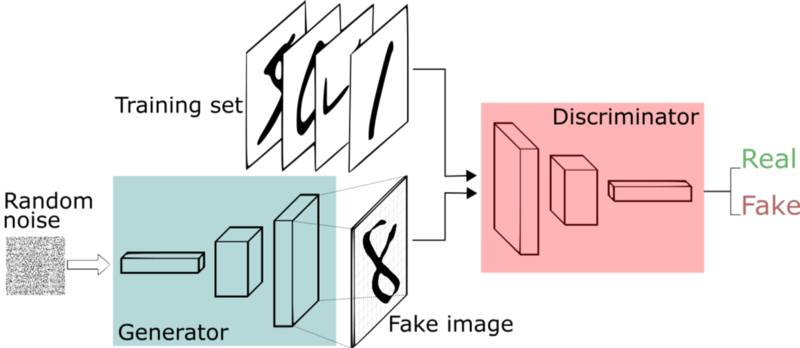
\includegraphics[width=0.7\textwidth]{images/gan.png}
		\caption{}
		\label{fig:gan_arch}
	\end{subfigure}
	\begin{subfigure}[b]{1.\textwidth}
		\centering
		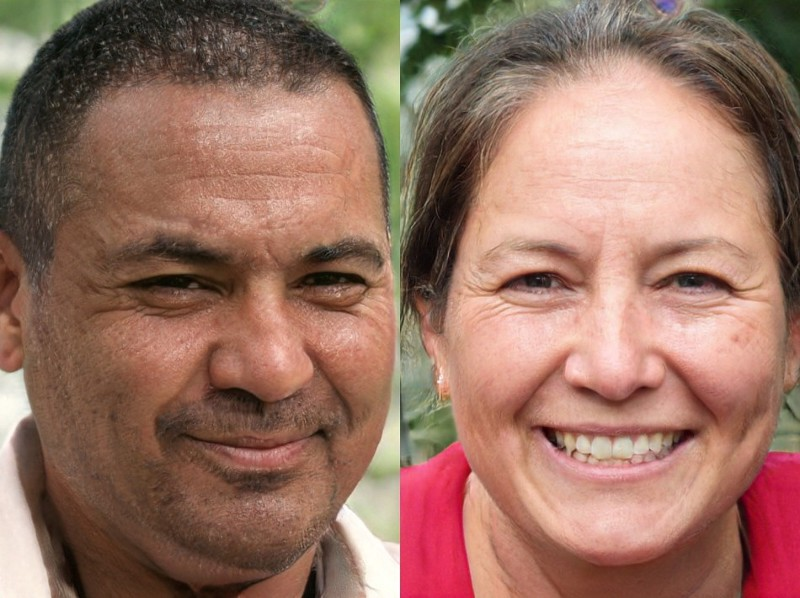
\includegraphics[width=0.5\textwidth]{images/Nvidia/SelectedGenerated.png}
		\caption{}
		\label{fig:gan_sample}
	\end{subfigure}
	\caption{
		روند کلی \gan{}
		(\subref{fig:gan_arch})
		و نمونه تصاویر تولید شده توسط این روش (\subref{fig:gan_sample})
		\cite{gan_nvidia}
	}
\end{figure}
شمایی از نحوه عملکرد این روش در شکل \ref{fig:gan_arch} آمده است؛ همچنین تصاویر شکل \ref{fig:gan_sample} توسط چنین شبکه‌ای تولید شده است که تصاویر بسیار طبیعی هستند.
\\
همان طور که در شکل \ref{fig:gan_arch} مشخص است، شبکه مولد،
\trans{\noise{}}{Noise}
را به تصویر تولید می‌کند. در واقع عامل تصادفی در تصادفی بودن \noise{} اولیه نهفته است. اما در حوزه متن معمولا مدل‌های مولد \noise{}‌ای را دریافت نمی‌کنند چرا که عامل اصلی در نمونه‌گیری هر کلمه در هر زمان وجود داشته و چندان نیازی به \noise{} ورودی نیست.
\section{چالش‌ها} \label{chap1:challenge}
\subsection{ 
    رفتار \meanseeking{} روش \maxlikelihood{}}
از آنجا که در روش \maxlikelihood{} در واقع فاصله $KL(\prob_\text{Data} ~ || Q)$ را کمینه می‌کنیم (زمانی که به دنبال یادگیری $Q$ هستیم)، لازم است تا رفتار مدل در حالتی که ظرفیتی کمتر از پیچیدگی داده دارد را بررسی کنیم. رفتار این فاصله، به گونه‌ای است که Q را به سمتی سوق می‌دهد تا به تمام نقاطی که در $\prob_\text{Data}$ احتمالی دارند، احتمالی نسبت دهد؛ اما نکته نامطلوب آن است که در صورت کمتر بودن ظرفیت مدل نسبت به پیچیدگی داده، برای احتمال نسبت دادن به تمام نقاط داده آموزشی، به نقاطی که در توزیع اصلی داده، احتمالی ندارند نیز احتمال نسبت می‌دهد.
\begin{figure}[h]
	\centering
	\begin{subfigure}[t!]{.4\textwidth}
		\centering
		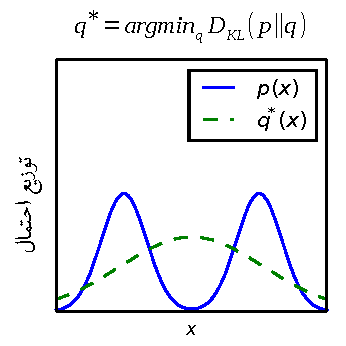
\includegraphics[height=1.\textwidth]{images/KLvsReverseKL_KL.pdf}
		\caption{}
		\label{fig:meanseeking_KL}
	\end{subfigure}
	\begin{subfigure}[t!]{.4\textwidth}
		\centering
		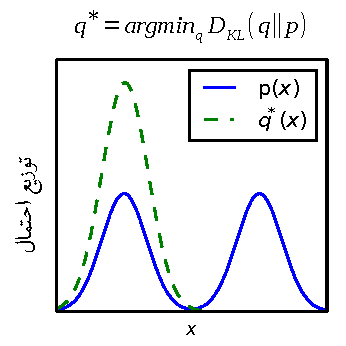
\includegraphics[height=1.\textwidth]{images/KLvsReverseKL_RKL.pdf}
		\caption{}
		\label{fig:meanseeking_RKL}
	\end{subfigure}
	\caption{
		تفاوت رفتار فاصله \lr{KL} (\subref{fig:meanseeking_KL}) و \lr{KL} برعکس (\subref{fig:meanseeking_RKL}) در نحوه یادگیری مدل.
	}
\end{figure}
همان طور که در شکل \ref{fig:meanseeking_KL} دیده می‌شود، ممکن است نقطه‌ای بیشینه احتمال داشته باشد که در توزیع اصلی احتمالی ندارد. به این رفتار روش \maxlikelihood{}، رفتار 
\trans{\meanseeking{}}{Mean Seeking}
 گفته می‌شود. این درحالیست که \lr{KL} برعکس، رفتاری معکوس داشته و در این حالت تنها یکی از قله‌ها را پوشش خواهد داد.
\subsection{ناپایداری و مشکلات \gan{}}
دو مشکل در نحوه آموزش \gan{} نهفته است. اول آنکه با توجه به نحوه آموزش مولد، تنها کافیست مولد نمونه‌ای تولید نماید که \discriminator{} توانایی تشخیص آن از نمونه واقعی را ندهد. در واقع طبیعی بودن نمونه‌ها در روش دیده شده است اما تنوع خیر؛ از سوی دیگر می‌تواند این رفتار به صورت تناوبی بین بعضی نمونه‌ها در حین آموزش جابه‌جا شود. برای مثال اگر هدف یادگیری تصویر قرمز رنگ شکل \ref{fig:gan_train} باشد، ممکن است مسیر آموزش به حالت شکل \ref{fig:gan_bad_train} درآمده و بین بعضی قله‌های داده جابه‌جا شود و از سوی دیگر نیز ممکن است به صورت شکل \ref{fig:gan_good_train} آموزش داده شود که حالتی پایدار است. اگر روند آموزش دچار چنین مشکلی شود، مدل دچار
\trans{\modecollapse{}}{Mode Collapse}
شده است \cite{wgan, gan}.
\begin{figure}[h]
	\centering
	\begin{subfigure}[h]{.7\textwidth}
		\centering
		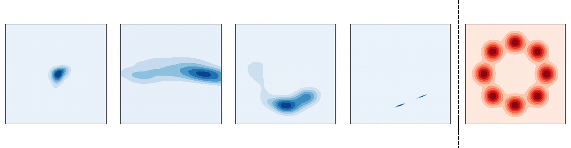
\includegraphics[width=1.\textwidth]{images/GANBadTrain.pdf}
		\caption{}
		\label{fig:gan_bad_train}
	\end{subfigure}
	\begin{subfigure}[h]{.7\textwidth}
		\centering
		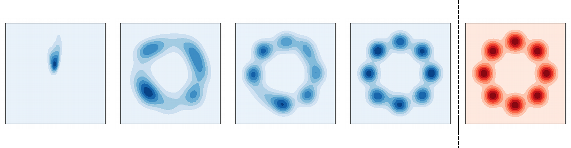
\includegraphics[width=1.\textwidth]{images/GANGoodTrain.pdf}
		\caption{}
		\label{fig:gan_good_train}
	\end{subfigure}
	\caption{
		نمونه‌ای آموزش ناپایدار (\subref{fig:gan_bad_train}) و پایدار
		(\subref{fig:gan_good_train}) \gan{} \cite{numerics_gan}5.
	}
	\label{fig:gan_train}
\end{figure}
\\
مشکل دوم نیز کنترل میزان آموزش \discriminator{} و \generator{} در مقابل یکدیگر است. در صورتی که \discriminator{} بیش از حد آموزش داده شود به طوری که به راحتی نمونه‌های واقعی را از مصنوعی تشخیص دهد، گرادیانی از \discriminator{} به مولد منتقل نشده و آموزش شبکه متوقف خواهد شد. به منظور رفع این مشکل‌ها، راه حل‌های متفاوتی همچون \wgan{}
\LTRfootnote{\lr{Wasserstein Generative Adversarial Network (WGAN)}}
  ارائه شده است \cite{wgan}.
\subsection{عدم توجه به فضای نهان} \label{chap1:latent_ignore}
زمانی که از مدل‌های با فضای نهان استفاده می‌شود، به دنبال یافتن فضای نهانی تفسیرپذیر و تاثیرگذار بر روی خروجی \decoder{} هستیم؛ اما در صورت بالا بودن ظرفیت \decoder{} ممکن است مستقل از فضای نهان، توزیع داده اصلی را فرا بگیرد. در این صورت فضای نهان نه تفسیرپذیر و نه تاثیرگذار بر روی خروجی \decoder{} بوده و عملا با یک مدل زبانی بدون فضای نهان برابری خواهد کرد. این مشکل نیز مورد توجه محققان بوده و روش‌های متفاوتی از جمله \wae{}
 \LTRfootnote{\lr{Wasserstein Autoencoder (WAE)}}
  ارائه شده است \cite{wae, infovae, vae_lagging, vae_lossy}.
\subsection{گذر گرادیان در نمونه‌برداری و \argmaxphrase{}}
از آنجا که در حوزه مدل زبانی با نمونه‌گیری از توزیع کلمات سر و کار داریم، در روش‌هایی مانند \gan{} با مشکل مواجه خواهیم بود. در واقع به دلیل اینکه نمونه‌گیری عملیاتی مشتق نا‌پذیر است، امکان گذر گرادیان از این عملیات به عقب وجود ندارد. برای مثال در روش \gan{}، تابع هدف مدل مولد، تولید نمونه‌هاییست که از نظر \discriminator{} واقعی به نظر رسند. بنابراین بایستی از مولد نمونه‌برداری کرده و سپس احتمال واقعی بودن نمونه‌ها توسط \discriminator{} ارزیابی شود. حال برای آموزش دادن پارامتر‌های مولد نیاز است تا گرادیان از \discriminator{} به مولد منتقل گردد؛ اما در این مسیر عملیات نمونه‌برداری وجود دارد. مشکل مشابهی نیز هنگام 
\trans{\argmaxphrase{}}{Argmax}
 رخ می‌دهد. برای رفع این مشکل نیز راه‌حل‌هایی همچون بهره‌گیری از یادگیری تقویتی و یا روش‌هایی تقریبی همچون \lr{Gumbel Softmax} و \lr{Soft-argmax} ارائه شده‌اند اما روش یادگیری تقویتی واریانس گرادیان را افزایش داده و روش‌های تقریبی نیز دارای پارامتر‌هایی هستند که تنظیم آن‌ها نیازمند توجه و دقت است \cite{seqgan, gumbel}
\subsection{عدم تطابق شرط با جمله تولیدی}
مشکل دیگری که ممکن است در روش‌های مبتنی بر \likelihood{} پیش آید، احتمال ناهمخوانی شرط با جمله تولیدی است. از آنجا که معمولا تطابق جمله خروجی با شرط چک نمی‌شود، ممکن است این اتفاق نامطلوب رخ دهد. لازم به ذکر است که در روش \gan{} انتظار چنین رخدادی وجود ندارد چرا که این موضوع توسط \discriminator{} تصحیح می‌شود \cite{toward}.
\section{هدف پژوهش}
با توجه به تعریف مسئله در بخش \ref{chap1:prob_define} و چالش‌های معرفی شده در بخش \ref{chap1:challenge} به دنبال ارائه روشی برای آموزش شبکه‌های مولد شرطی بوده که کمتر با چالش‌های ارائه شده مواجه شود و جملات تولیدی چه به لحاظ کیفیت و چه به لحاظ تطابق با شرط از سطح قابل قبولی برخوردار باشند.
\\
به این منظور در یک رویکرد، سعی در آموزش مدل مولد با فضای نهان شرطی به طوری که فضای نهان به ازای مقادیر مختلف شرط تقسیم گردد، خواهیم داشت؛ اما در رویکرد دوم، فضای نهان از شرط 
\trans{مستقل}{Disentangle}
بوده و نسبت به مقادیر مختلف شرط تقسیم نخواهد شد. علاوه بر این از معماری‌های نوینی همچون \transformer{}، روش‌هایی همچون \wae{} برای جلوگیری از مشکل عدم توجه به فضای نهان و همچنین رویکرد‌های آموزش مدل‌های مولدی که کمتر مورد توجه بوده‌اند اما ویژگی‌های متناسب با فضای مسئله را دارند، استفاده خواهد شد.

\section{ساختار پایان‌نامه}
در فصل \ref{chap2}، پس از معرفی تعدادی فاصله بین توزیع‌های به عنوان پیشنیاز، به دلیل شباهت مدل‌های زبانی شرطی به غیر شرطی، ابتدا مدل‌های غیر شرطی تحت عنوان مدل‌های با فضای نهان و بدون فضای نهان تشریح شده و در انتها نیز معماری نوینی تحت عنوان \transformer{} معرفی می‌گردد. از آنجا که در روش پیشنهادی از نوعی مدل‌های مولد که پیش‌تر مورد توجه نبوده‌اند استفاده گردیده است، به معرفی این دسته از مدل‌های مولد نیز پرداخته خواهد شد. در فصل \ref{chap3} نیز پس از بررسی اجمالی مدل‌های معرفی شده، مدل پیشنهادی ارائه شده و در فصل  \ref{chap4} پس از معرفی داده و معیارهای ارزیابی مورد بررسی قرار گرفته و نتایج گزارش شده است. در نهایت نیز ضمن ارائه جمع‌بندی از کارهای انجام شده، پیشنهاداتی جهت ادامه تحقیقات معرفی خواهد شد.





\chapter{پژوهش‌های پیشین}\label{chap2}
\minitoc

\section{مقدمه}\label{intro}
در فصل قبل مقدمات کلی و تعریف مسئله مطرح شدند. در این فصل در ابتدا چندین فاصله، شامل فاصله‌های معروف و بعضی فواصلی که اخیرا با اقبال مواجه شده‌اند، توضیح داده خواهند شد. در ادامه، بعضی مدل‌های زبانی با فضای نهان و در ادامه مدل‌های زبانی بدون فضای نهان، نوعی از شبکه‌ها که به \normalizingflownets{} معروف هستند، معرفی خواهد شد. در نهایت نیز مدل‌های زبانی شرطی شرح داده خواهند شد.
\subsection{پیش‌نیازها}
\iffalse
	قرارداد می‌کنیم توزیع $P$ مربوط به توزیع داده واقعی باشد و در مقابل آن به دنبال یافتن توزیع $Q$ هستیم که تا حد ممکن نزدیک به $P$ باشد.
	از آنجا که در طول متن گزارش، فاصله‌های گوناگونی مورد استفاده قرار گرفته است، در ابتدا آن‌ها تعریف می‌کنیم. در تمامی تعاریف، P مربوط به توزیع اصلی و Q مربوط به توزیعی است که یاد گرفته می‌شود.
\fi
\subsubsection{معیارهای فاصله بین دو توزیع} \label{chap2:divs}
پیش از توضیح روش‌های مختلف ابتدا  لازم به ذکر است تمامی این فواصل بین دو توزیع $p$ و $q$ تعریف شده‌اند.
\\
\bff{فاصله \lr{KL}} \cite{bishop}:
\begin{gather} \label{eq: kl}
	KL (p ~ || ~ q)   = \sum_x p(x) \log \frac{p(x)}{q(x)}
\end{gather}
اگر $p$ توزیع داده باشد و به دنبال یادگیری $q$ باشیم، کمینه کردن فاصله فوق همان روش \maxlikelihood{} خواهد بود.
\\
\bff{فاصله \lr{KL} برعکس}:
\begin{gather} \label{eq: rkl}
	KL (q ~ || ~ p)   = \sum_x q(x) \log \frac{q(x)}{p(x)}
\end{gather}
مجددا اگر $p$ توزیع داده باشد، از آنجا که دسترسی به آن وجود ندارد، فاصله فوق به صورت مستقیم قابل بهینه‌سازی نیست.
\\
\bff{فاصله \lr{Jensen Shannon}}:
\begin{gather} \label{eq: js}
	JS (p ~ || ~ q)   = KL(p ~ || ~ \frac{p + q}{2}) + KL(q ~ || ~ \frac{p + q}{2})
\end{gather}
این فاصله بر خلاف دو فاصله قبلی، نسبت به جابه‌جایی $p$ و $q$ حساس نبوده و \gan{} در تئوری، این فاصله را کمینه می‌کنند \cite{gan}.
\\
\bff{فاصله
	\trans{\wasser{}}{Wasserstein}}:
فرض کنید می‌خواهید تعداد مشخصی جعبه که به ترتیب خاصی بر روی یکدیگر و کنار هم قرار گرفته‌اند را به مکانی دیگر منتقل کنید. برای مثال طبق شکل \ref{fig:chap2:wasser1} میخواهید مربع‌های سمت چپ را به مکان‌های با نقطه‌چین مشخص شده منتقل کنید. به صورت‌های مختلفی می‌توان این کار را انجام داد. دو نمونه از این جابه‌جایی در شکل \ref{fig:chap2:wasser2} آمده است.
\begin{figure}[h]
	\centering
	\begin{subfigure}[t]{.7\textwidth}
		\centering
		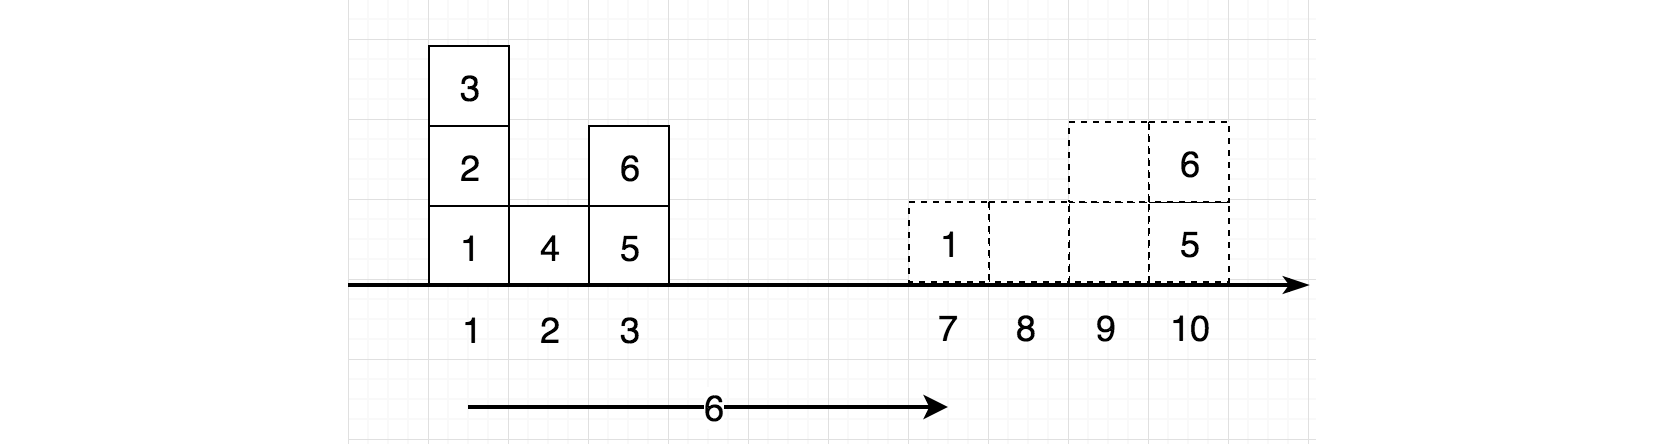
\includegraphics[width=1.\textwidth]{images/wasser2.png}
		\caption{}
		\label{fig:chap2:wasser1}
	\end{subfigure}

	\begin{subfigure}[t]{.6\textwidth}
		\centering
		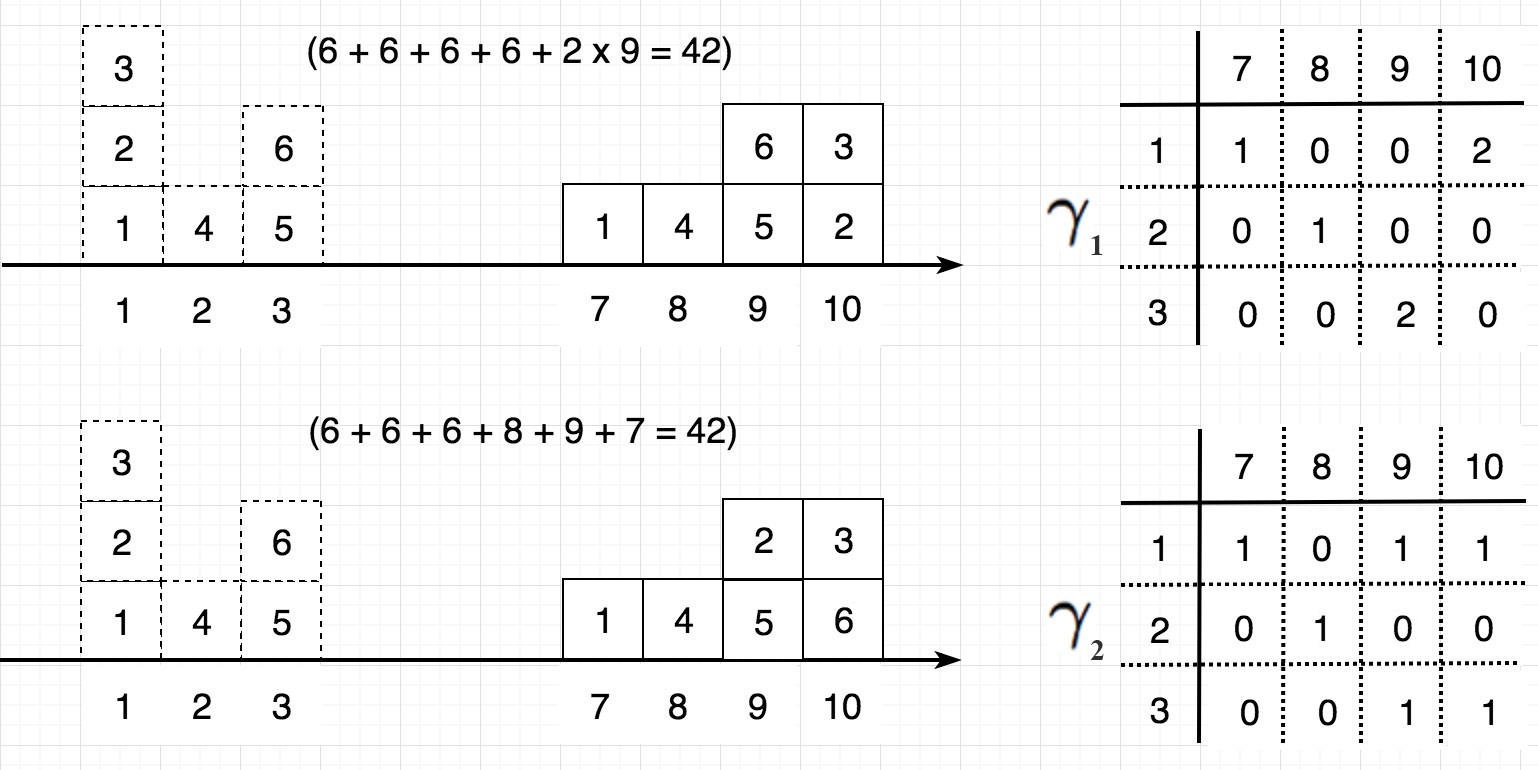
\includegraphics[width=1.\textwidth]{images/wasser1.jpeg}
		\caption{}
		\label{fig:chap2:wasser2}
	\end{subfigure}
\caption{
    مثالی از دو توزیع \subref{fig:chap2:wasser1} و 
    \transportplan{} 
    بین دو توزیع \subref{fig:chap2:wasser2}}
\end{figure}
اگر $\gamma$ را یک
\trans{\transportplan{}}{Transport Plan}
بنامیم که به صورت جدولی که سطرها مکان اولیه جعبه‌ها و ستون‌ها مکان ثانویه جعبه‌ها نشان داده و هر خانه آن نشان دهنده تعداد جعبه‌ی جابه‌جا شده از نقطه اولیه به ثانویه است، جمع عناصر این جدول برابر هزینه جابه‌جایی کلیه جعبه‌ها خواهد بود. از آنجا که \transportplan{} واحدی به این منظور وجود ندارد، \transportplan{} با کمترین هزینه جابه‌جایی برابر فاصله \wasser{} بین حالت اولیه و ثانویه جعبه‌ها است.
\\
به منظور تعریف دقیق‌تر، اگر دو توزیع به نام‌های $q$ و $p$ داشته باشیم، فاصله \wasser{} برابر کمترین هزینه جابه‌جایی برای جابه‌جایی جرم توزیع $p$ به $q$ خواهد بود.
اگر مجموعه تمام توزیع‌های توام $\gamma(x,y)$ که توزیع‌های \marginal{} آن به ترتیب برابر $p$ و $q$ باشد را با $\Pi(p,q)$ نشان دهیم، فاصله \wasser{} به صورت زیر تعریف می‌شود:
\begin{align}
	W_c(p,q) = \inf_{\gamma(x,y) \in \Pi(p,q)} \expected_{(x,y) \sim \gamma(x,y)} [ c(x,y) ]
\end{align}
و $c$ یک متر تعریف شده بر روی این فضا و اندازه‌گیرنده هزینه جابه‌جایی بین دو نقطه است. به طور شهودی توزیع توام $\gamma$ نشان دهنده جرم جابه‌جا شده از نقطه $x$ به نقطه $y$ است به طوری که تمام جرم از توزیع $p$ به توزیع $q$ منتقل شود. در حالتی که $c = ||x-y||$ باشد، به فاصله فوق فاصله \earthmover{} نیز گفته می‌شود.
\\
از آنجا که کمینه کردن فاصله فوق معمولا سخت است، طبق فرم دوگان \lr{Kantorovich-Rubinstein } فاصله \earthmover{} برابر است با \cite{wgan}:
\begin{align}
	W(p, q) = \sup_{||f||_L \leq 1} \expected_{x \sim p(x)}[f(x)] - \expected_{x \sim q(x)}[f(x)]
\end{align}
که سوپریمم بر روی تمام توابع $f$ با ضریب \lipschitz{} حداکثر یک گرفته شده است. شرط \lipschitz[K-]{} که به صورت
$|f(x) - f(y)| \leq K |x - y|$
به ازای تمام $x$ و $y$ ها تعریف می‌شود به طور شهودی به معنای توابعی است که چندان تغییرات شدیدی ندارند.
\\
از این فاصله به عنوان تابع هدف جدید در \gan{} استفاده شده که به \wgan{} معروف است. نکته قابل توجه این است که چون تابع $f$ فوق چندان انحنای شدیدی ندارد، حتی در صورت دور بودن توزیع داده واقعی و مصنوعی، همچنان تابع $f$ به صورت محلی احتمالا خطی بوده و گرادیان از \discriminator{} به \generator{} بر خواهد گشت \cite{wgan}. نمایی از این تفاوت گرادیان دو نوع  \gan{} در شکل \ref{fig:chap2:wgan1} مشخص است.
\begin{figure}[h]
	\centering
	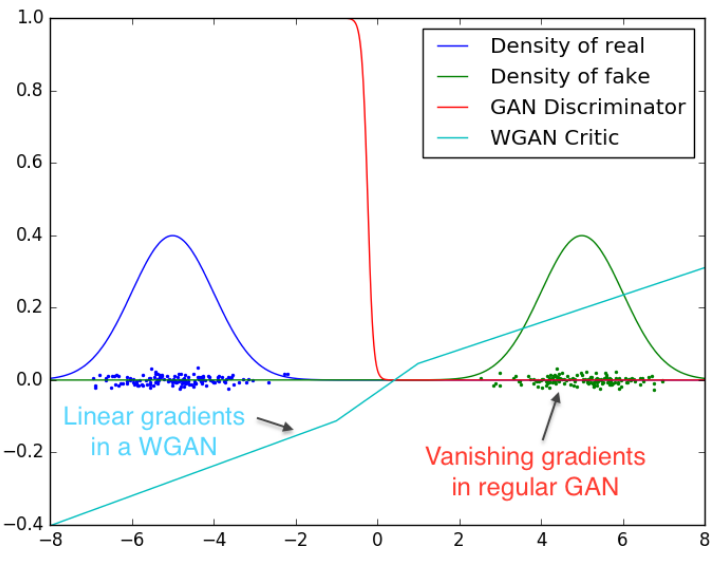
\includegraphics[width=0.5\textwidth]{images/wgan1.png}
	\caption{
        تفاوت خروجی \discriminator{} در \gan{} عادی و \wgan{} (\lr{WGAN})
        \cite{wgan}
    }
	\label{fig:chap2:wgan1}
\end{figure}
\\
\bff{فاصله 
    \trans{بیشینه اختلاف میانگین}{Maximum Mean Disrepancy (\mmd{})} (\mmd{})}:
برای تابع کرنل مثبت معین 
\trans{‎\reproducing{}}{Reproducing}
$k: ‎\mathcal{Z} ‎‎\times \mathcal{Z} ‎\rightarrow ‎\mathbb{R}‎‎$
رابطه ‎\mmd{} به شکل زیر تعریف می‌شود:
\begin{gather}
	\mathsf{MMD}_k(p, q) = {\vert \vert \int_\mathcal{X} k(x, .) dp(x) - \int_\mathcal{X} k(x, .) dq(x) \vert \vert}_{\mathcal{H}_k}
\end{gather}
به طوری که $‎\mathcal{H}‎_k$، یک 
\trans{کرنل \reproducing{} در فضای هیلبرت}{Reproducing ‎ Kernel ‎ Hilbert ‎ Space (RKHS)}،
برای توابع از $‎\mathcal{X}‎$ به اعداد حقیقی است. اگر تابع $k$ ویژگی‌های مشخصی را داشته باشد، ‎\mmd{}‎ را به یک متر تبدیل کرده و این امکان را فراهم می‌کند تا از این متر به عنوان تابع هزینه برای کمینه کردن فاصله دو توزیع $p$  و $q$  بهره برده شود. از آنجا که رابطه بالا به طور مستقیم قابل محاسبه و بهینه‌سازی نیست، از تخمین‌گر 
\trans{نااریب}{Unbiased}
 زیر استفاده می‌گردد. اگر $n$ نمونه از دو توزیع $p$ و $q$ داشته و به ترتیب با $x_i$ و $‎\tilde{x}_i$ نشان داده شوند،‌خواهیم داشت:
\begin{align}
	\mathsf{MMD}_k(x_{1,2,...,n};\tilde{x}_{1,2,...,n}) = & \frac{1}{n(n-1)} \sum_{l \neq j} k(x_l, x_j) +
	\frac{1}{n(n-1)} \sum_{l \neq j} k(\tilde{x}_l, \tilde{x}_j)                            \nonumber         \\
	                                                      & - \frac{1}{n ^ 2} \sum_{l, j} k(x_l, \tilde{x}_j)
\end{align}
فاصله فوق با کرنل
$k(x, y) = \frac{C}{C + ||x - y||^2_2}$
برای فاصله بین دو توزیع گاوسی کاربرد دارد و به خوبی عمل می‌کند \cite{wae}.

\section{مدل‌های زبانی بدون فضای نهان}
\subsection{مدل زبانی پایه (\teacherforcing{})}
مدل \teacherforcing{} شاید ساده‌ترین دسته از مدل‌های تولید متن با استفاده از شبکه‌های عصبی باشد. آموزش این مدل‌ها مبتنی بر بیشینه کردن \likelihood{} داده آموزش در مدل است \cite{teacher_force} اگر پارامترهای مدل را با $‎\theta$ نشان دهیم، تابع هزینه این مدل به صورت زیر است:
\begin{equation}\begin{split}
		L_{MLE} = -\expected_{\bff{x} \sim p_{data}(\bff{X})} [\log p_\theta (\bff{x})] = -\expected_{\bff{x} \sim p_{data}(\bff{X})} [\log p_\theta (\bff{x}_1) + \sum_{t=2}^{T}  \log p_\theta (\bff{x}_t|\bff{x}_1, ..., \bff{x}_{t-1})].
	\end{split}\end{equation}

\begin{figure}[H]
	\centering
	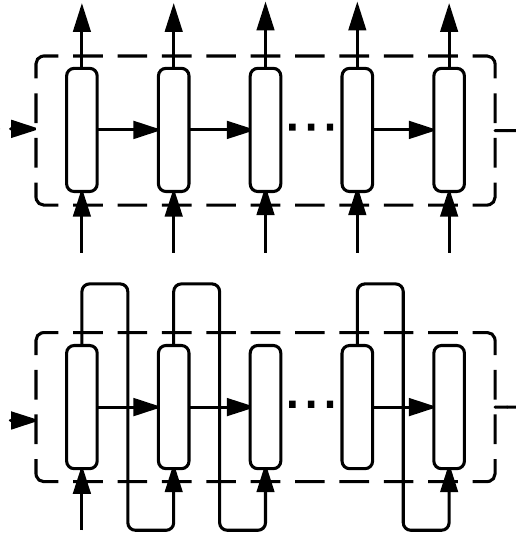
\includegraphics[width=0.25\textwidth]{images/teach-prof.png}
	\caption{
		تفاوت بین آموزش و آزمون مد‌ل جبر معلم. شکل بالا مربوط به زمان آموزش و شکل پایین مربوط به زمان آزمون است. \cite{prof_force}.}
	\label{fig:chap2:expbias}
\end{figure}

به عبارت دیگر، در هر زمان درست‌نمایی هر کلمه را با داشتن کلمات قبلی بیشینه می‌کنیم. \\
همان‌طور که از روابط تابع هزینه مشخص است، آموزش این دسته از مدل‌ها ساده بوده اما دچار پدیده‌ای به نام 
\trans{اریبی مواجهه}{Exposure bias}
 هستند \cite{ prof_force, s_sampling}. این مشکل ناشی از تفاوت رفتار با مدل حین آموزش و حین آزمون است. همان طور که در شکل \ref{fig:chap2:expbias} مشخص است، حین آموزش، در هر زمان، کلمات کاملا درست تحویل مدل شده، در حالی که در زمان آزمون ورودی شبکه در هر زمان، با استفاده از نمونه‌گیری از خود مدل در زمان قبل ساخته می‌شود. از آنجا که مدل مفهوم کاملا درستی را نیاموخته است، کلمه‌ی تولید شده برای ورود به زمان بعد، کلمه کاملا صحیحی نبوده و چنین رفتاری باعث می‌شود تا مدل، ورودی‌ای را دریافت کند که دارای مقداری خطا بوده که در زمان آموزش مانند آن را ندیده است (در زمان آموزش کلمات کاملا صحیح ورودی شبکه بوده‌اند)؛ این رفتار در طول تولید هر کلمه از یک جمله با هم تجمیع شده و در نهایت منجر به تولید جمله‌ای نه چندان صحیح خواهد شد.\\
به منظور رفع این مشکل، روش‌های متفاوتی ارائه شد \cite{prof_force, s_sampling, seqgan} که در بخش \ref{chap2:seqgan} به عنوان یکی از راه‌حل‌ها به آن پرداخته خواهد شد.
از دیگر مشکلات این روش باید به تفاوت تابع هزینه و معیار ارزیابی اشاره کرد؛ به عبارت دیگر اگر معیار ارزیابی، معیاری مانند \lr{BLEU} باشد، هدف ارزیابی کسب امتیاز بالاتر \lr{BLEU} است و نه افزایش درست‌نمایی داده آموزش و لزوما افزایش درست‌نمایی به افزایش ‌\lr{BLEU} منجر نمی‌شود.
\subsection{مدل زبانی با استفاده از \gan{}}
شاید 
\trans{‎\gan}{Generative adversarial networks}
 یکی از مطرح‌ترین و موفق‌ترین مدل‌های مولد حال حاضر باشند. این شبکه‌ها که مجددا ابتدا در حوزه تصویر معرفی شدند، از دو بخش کلی تشکیل شده اند \cite{gan}؛ بخش 
\trans{مولد}{Generator}
  و بخش 
\trans{\discriminator}{Discriminator}.
  همان‌طور که از نام‌گذاری آن‌ها مشخص است، مولد وظیفه تولید نمونه‌های مصنوعی و \discriminator{} وظیفه تشخیص نمونه مصنوعی از واقعی را دارد. نحوه آموزش آن‌ها به این صورت است که مولد سعی در تولید نمونه‌های شبیه به داده واقعی داشته و \discriminator{} در جهت مخالف سعی در شناسایی این نمونه‌ها دارد. در واقع نوعی 
\trans{بازی کمینه-بیشینه}{Min-max game}
بین مولد و \discriminator{} در جریان است. تابع هدف این مدل به شرح زیر است \cite{gan}:
\begin{equation} \label{eq:gan}
	\begin{split}
		V_{GAN} (G, D) = \expected_{\bff{x} \sim p_{data}(\bff{X})} [\log D(\bff{x})] + \expected_{\bff{z} \sim p(\bff{Z})} [\log (1 - D(G(\bff{z})))]
	\end{split}
\end{equation}
که  $p(\bff{z})$ توزیع پیشین تعریف شده بر روی نویز $\bff{z}$،
$G(\bff{z})$
تابع مولد (تبدیل کننده نویز $\bff{z}$ به نمونه $\bff{x}$)، $D(\bff{x})$ تابع \discriminator{} بوده و این رابطه برحسب $G$ کمینه و $D$ بیشینه می‌گردد.\\
اگر $q_G(\bff{x})$ نشان دهنده توزیع حاصل از اعمال تابع $G(\bff{z})$ به توزیع پیشین $p(\bff{z})$ باشد؛ نشان داده شده است که نقطه بیشینه کننده رابطه \ref{eq:gan} بر حسب $D$، به صورت زیر است \cite{gan}:
\begin{gather}
	D_G^*(\bff{x}) = \frac{p_{data}(\bff{x})}{p_{data}(\bff{x}) + q_G(\bff{x})}
\end{gather}
با فرض رسیدن به \discriminator{} بهینه، کمینه کردن $V(D^*_G,G)$ معادل کمینه کردن فاصله \lr{Jensen Shannon} بین $p_{data}(\bff{x})$ و $q_G(\bff{x})$ خواهد بود.

همان طور که اشاره شد \gan{}، ابتدا در حوزه تصویر معرفی شده و به دلیل عدم امکان عبور گرادیان که در ادامه شرح داده خواهد شد، چندان در حوزه متن موفق نبود. این مشکل از نحوه آموزش نشأت می‌گیرد. همان طور که در روابط تابع هزینه مشخص است، \discriminator{} باید به نمونه‌های تولید شده توسط مولد عددی نزدیک به صفر نسبت دهد. آنچه که باید در آموزش و الگوریتم 
\trans{گرادیان کاهشی تصادفی}{Stochastic gradient descent}
محاسبه شود، محاسبه مشتق تابع هزینه نسبت به پارامتر‌های شبکه مولد است؛ اما از آنجا که شبکه مولد مستقیما در تابع هزینه شرکت نکرده و نمونه‌های تولیدی آن شرکت می‌کنند و عملیات نمونه‌گیری در فضای گسسته عملیاتی مشتق‌ناپذیر است، بنابراین امکان گذر گرادیان از تابع هزینه (شبکه \discriminator{}) به شبکه مولد به سادگی وجود ندارد. در واقع شبیه چنین مشکلی در شبکه‌های \vae{} نیز وجود دارد اما با تکنیکی به نام
\trans{\reparametrization{}}{Reparameterization}
که منبع تزریق عامل تصادفی (نمونه‌گیری) را از مسیر انتقال گرادیان خارج می‌کند، حل شده است \cite{vae}.\\
به منظور حل این مشکل نیز رویکرد‌های متفاوتی ارائه شده است که به یکی و شاید معروف‌ترین از آن‌ها اشاره خواهد شد \cite{seqgan, gumbel}.\\
\subsubsection*{\lr{SeqGAN}}  \label{chap2:seqgan}
در روش \lr{SeqGAN} راه حل ارائه شده برای مشکل گذر گرادیان الهام گرفته شده از حوزه 
\trans{یادگیری تقویتی}{Reinforcement Learning}
است \cite{seqgan}؛ در واقع همین مشکل به نوعی دیگر در حوزه یادگیری تقویتی مطرح است و با روشی به نام روش \trans{گرادیان سیاست}{Policy gradient} رفع شده است. ساختار یک مسئله حوزه یادگیری تقویتی شامل ۴ بخش است که با تعریف تمام بخش‌های آن، ‌می‌توان بخش آموزش مولد در \gan{} را به عنوان آموزش یک عامل با روش \reinforce{} دید. این بخش‌ها شامل موارد روبرو هستند: فضای حالت عامل ($S$)، فضای عمل عامل ($A$)، 
\trans{تابع گذار}{Transition function}
(\lr{$T(s,a)$})
و 
\trans{تابع پاداش}{Reward function}
(\lr{$R(s,a)$}).
\begin{equation}\begin{split}
		\nonumber
		T: S \times A \rightarrow S\\
		R: S \times A \rightarrow \mathbb{R}
	\end{split}\end{equation}
در اینجا حالت فعلی عامل، 
\trans{بازنمایی}{Representation}
کلمات تولید شده تا به حال است؛ عمل عامل،‌ کلمه انتخابی بعدی؛ حالت بعدی، تجمیع کلمات قبلی تولید شده و کلمه فعلی و در نهایت تابع پاداش، امتیاز میزان واقعی بودن جمله است که تمایز دهنده به جمله تولیدی نسبت می‌دهد. بدیهی است که تابع گذار تابعی 
\trans{قطعی}{Deterministic}
بوده و پاداش مورد نظر بعد از تولید کامل جمله به عامل داده می‌شود. در این حالت رابطه گرادیان تابع مولد به شکل زیر بدست خواهد آمد \cite{seqgan}.
\begin{equation} \label{eq:seqgan-grad}
	\begin{split}
		\nabla_G L_{GAN} (G, D) &= \nabla_G \expected_{\bff{x} \sim G(\bff{X})} [\log D(\bff{x})]= \expected_{\bff{x} \sim G(\bff{X})} [\log D(\bff{x}) \nabla_G \log G(\bff{x})].
	\end{split}
\end{equation}

\begin{figure}[t]
	\centering
	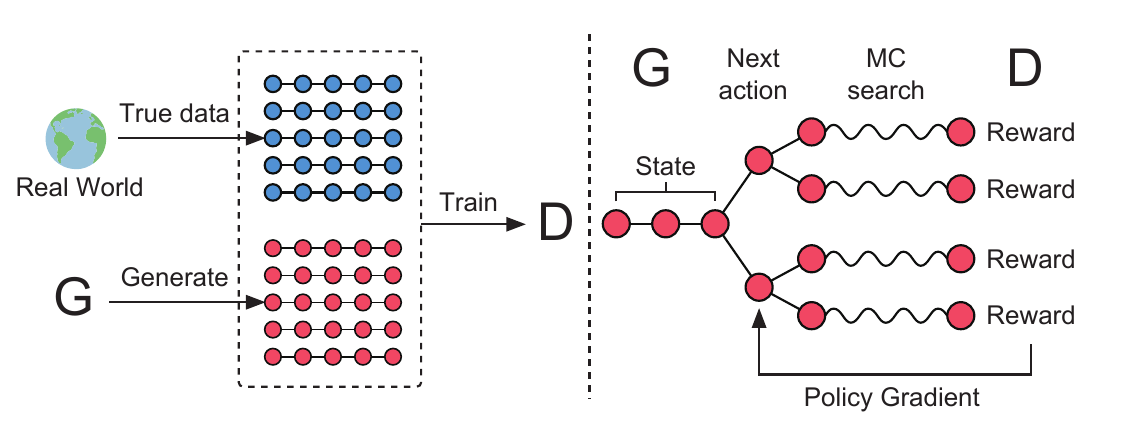
\includegraphics[width=0.5\textwidth]{images/seq-gan.png}
	\caption{
		نمایی نحوه آموزش مدل \lr{SeqGAN}
		\cite{seqgan}.}
	\label{fig:seq-gan}
\end{figure}

همان‌طور که در شکل \ref{fig:seq-gan} و رابطه \ref{eq:seqgan-grad} مشخص است، عامل طبق سیاستی که تا به حال بدست آورده است، تعدادی نمونه ایجاد نموده و به نسبت پاداش دریافتی به ازای هر نمونه، درست‌نمایی نمونه‌های مرتبط را افزایش خواهد داد.\\
نکته قابل توجهی که لازم است به آن اشاره شود، توانایی این روش در حل مشکل \expbias{} است. در واقع از یک سو در هر زمان کلمه بعدی توسط خود مدل تولید می‌شود و از سوی دیگر پاداشی که از \discriminator{} دریافت می‌کند، میزان  واقعی بودن کل جمله است؛ بنابراین اگر جمله تولید شده از نظر \discriminator{}، کیفیت لازم را نداشته باشد، \discriminator{} امتیاز کمتری به آن نسبت خواهد داد و گرادیان متناسب به مولد اعمال خواهد شد. با وجود آنکه این روش مشکل ذکر شده را حل می‌کند، اما فضایی که عامل باید در آن به دنبال یافتن پاداش بیشینه باشد نمایی بوده و همین امر آموزش این دسته از مدل‌ها را با چالش روبرو می‌کند. پیشنهاد ساده‌ای که برای این موضوع ارائه می‌شود استفاده از پیش آموزش به روش \teacherforcing{} است. در واقع ابتدا مدل به یک 
\trans{بهینه محلی}{Local optimum}
رسیده و در فضای نزدیک به آن احتمالا پاداش بیشتری نسبت به حالتی که مدل تصادفی باشد دریافت کرده و به اصلاح خود می‌پردازد.\\
این روش تنها مدل موجود با چنین رویکردی نبوده و روش‌هایی همچون \cite{pg_bleu} از دانش خبره مانند معیار \lr{BLEU} به عنوان پاداش بهره برده‌اند.
\section{مدل‌های زبانی با فضای نهان}
\subsection{خودکدنگار وَردِشی}
با معرفی \vae{}،
موج جدیدی در حوزه مدل‌های مولد به طور خاص مدل‌های مولد تصویر ایجاد شد.
\begin{figure}[H]
	\centering
	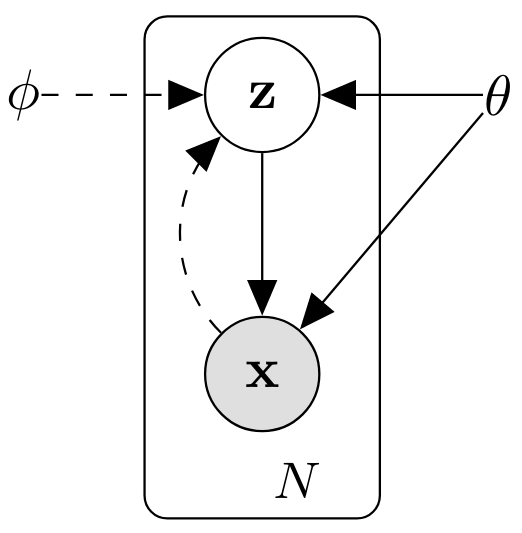
\includegraphics[width=0.25\textwidth]{images/vae-pgm.png}
	\caption
    [نمایی از مدل گرافی مورد استفاده در \vae{}.]
    {
		نمایی از مدل گرافی مورد استفاده در \vae{}. خطوط خطچین‌‌دار مربوط به تخمین توزیع پسین $p_\theta(\bff{z}|\bff{x})$ و خطوط بدون خطچین مربوط به مدل مولد
		$p_\theta(\bff{x}|\bff{z})$
		است.
		\cite{vae_text}.}
	\label{fig:vae-pgm}
\end{figure}
این ساختار به منظور یادگیری و 
\trans{\inference{}}{Inference}
مدل‌های با مدل گرافی نشان داده شده در شکل ‎\ref{fig:vae-pgm}‎ ارائه شده است. در واقع در این مدل، هر داده از یک \trans{\latentvar{}}{Latent Variable}  تولید شده که \priordist{} مشخصی برای آن تعریف شده است و معمولا توزیع گاوسی نرمال است. از آنجا که محاسبه $\log p_\theta(\bff{x})$ و $\log p_\theta (z|x)$ نیازمند \inference ی 
\trans{سخت}{Intractable}
است، با بهره‌گیری از  توزیع وردشی $q_\phi(z|x)$، کران پایینی از \likelihood{} به نام \lr{ELBO} بیشینه می‌گردد.\\
از دیدگاهی دیگر، این مدل از دو بخش کلی تشکیل شده است؛ \encoder{} و \decoder{}. بخش \encoder{} وظیفه کد کردن داده ورودی در فضای نهان را داشته و در مقابل \decoder{} وظیفه برگرداندن فضای نهان به داده اصلی. تفاوت این مدل‌ها با \autoencoder{}ها در فرض و اعمال توزیع نرمال بر فضای نهان است؛ به همین دلیل امکان نمونه‌برداری از فضای نهان امکان‌پذیر خواهد بود. تابع هزینه در این ساختار، به شکل زیر تعریف شده است \cite{vae}:
\begin{equation} \label{eq:vae}
	\begin{split}
		L_{VAE} = \expected_{\bff{x} \sim p_{data}(\bff{X})} [KL(q_\phi(\bff{Z}|\bff{x}) || N(\textbf{\latin{0}},\textbf{\latin{I}}))- \expected_{\bff{z} \sim q_\phi(\bff{Z}|\bff{x})}[\log p_\theta(\bff{x}|\bff{z})]]
	\end{split}
\end{equation}
که $q_\phi(\bff{z}|\bff{x})$ تابع توزیع \encoder{} و $p_\theta(\bff{x}|\bff{z})$ تابع توزیع \decoder ست. همان طور که مشخص است، تابع هزینه از دو بخش کلی تشکیل شده است. قسمت اول وظیفه اجبار کردن تابع توزیع \encoder{} به کد کردن داده‌ها در فضای گاوسی نرمال و بخش دوم نیز وظیفه کمینه کردن خطای بازسازی داده ورودی را بر عهده دارد. بنابراین شبکه سعی در یادگرفتن مدلی دارد که علاوه بر داشتن خطای بازسازی کم، توزیع گاوسی نرمال نیز بر فضای نهان آن حاکم باشد؛ پس می‌توان بعد از آموزش مدل، با نمونه‌گیری از توزیع نرمال و کدگشایی آن توسط $p_\theta(\bff{x}|\bff{z})$ داده مصنوعی تولید نمود. از آنجا که معمولا از توزیع گاوسی نرمال به عنوان \priordist{} استفاده میگردد و خروجی \encoder{} نیز توزیعی گاوسی با ماتریس کوارایانس قطری است، عبارت $KL(q_\phi(\bff{Z}|\bff{x}) || N(\textbf{\latin{0}},\textbf{\latin{I}}))$ به صورت فرم بسته قابل محاسبه خواهد بود. نکته قابل توجه این است که طبق رابطه \ref{eq:vae}، سعی بر این است تا خروجی \encoder{} به ازای هر نقطه، مستقلا، به توزیع گاوسی نرمال نزدیک باشد؛ بنابراین این قسمت از تابع هزینه، محدودیت زیادی را بر روی خروجی \encoder{} اعمال کرده و همان طور که در آینده توضیح داده خواهد شد، فرآیند آموزش آن را در بعضی حوزه‌ها دچار مشکل می‌کند \cite{vae_text}. 
\\
\begin{figure}[H]
	\centering
	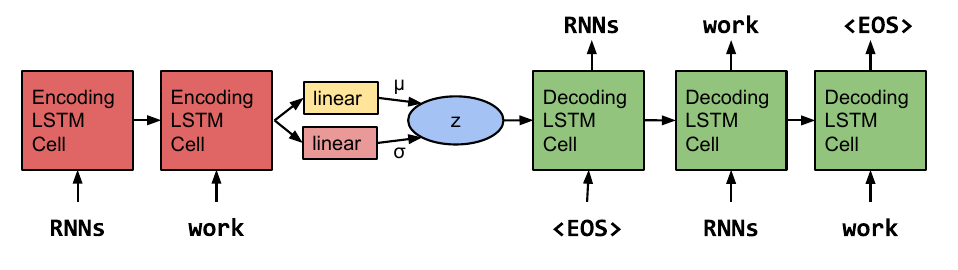
\includegraphics[width=0.5\textwidth]{images/vae-text.png}
	\caption{
		نمایی از مدل \vae{} استفاده شده در حوزه متن
		\cite{vae_text}.}
	\label{fig:vae-text}
\end{figure}
\label{chap2:latent_ignore}
آنچه که در حوزه متن اتفاق می‌افتد، صفر شدن قسمت شامل فاصله \lr{KL}  است؛ در واقع می‌توان این طور بیان کرد که کدگذار بدون توجه به معنی‌دار بودن فضای نهان، هر جمله را مستقلا به یک نقطه از فضای نهان نگاشت می‌کند. در نتیجه‌ی این روند، کدگشا هم مستقل از معنای فضای نهان جمله‌ای را تولید خواهد نمود و توزیع نرمال فرض شده بر فضای نهان یک جمله، چندان حاوی جملات مشابه آن نخواهد بود و روند آموزش به مشکل بر خواهد خورد. \\
یکی از راه‌کارهای اولیه به کار برده شده، دخیل کردن تدریجی قسمت حاوی \lr{KL} به تابع هزینه است. در واقع تابع هزینه به صورت زیر تغییر می‌کند:
\begin{equation}
	\begin{split}
		L_{VAE} = \expected_{\bff{x} \sim p_{data}(\bff{X})} [\lambda_{KL} KL(q(\bff{Z}|\bff{x}) || N(\textbf{\latin{0}},\textbf{\latin{I}}))- \expected_{\bff{z} \sim q(\bff{Z}|\bff{x})}[\log p(\bff{x}|\bff{z})]]
	\end{split}
\end{equation}
که $\lambda_{KL}$ ضریبی مثبت است. در واقع در ابتدا با قرار دادن $\lambda_{KL}=0$، مدل تنها یک خودرمزنگار ساده بوده و فضای نهان معنا داری ساخته و به مرور با میل دادن آن به یک، سعی در جمع کردن فضای نهان در فضای گاوسی نرمال خواهد داشت. جالب توجه است که چنین اتفاقی در حوزه تصویر رخ نمی‌دهد و قسمت \lr{KL} صفر نمی‌شود.
\iffalse
	این پدیده را شاید بتوان این طور توجیه کرد که از یک سو تغییرات ابتدایی فضای نهان زیاد بوده و دخیل کردن این تغییرات در تولید نمونه مورد نظر امری دشوار است؛ از سویی دیگر کدگشا به لحاظ معماری توانایی نگاشت هر نقطه از فضا را به جمله مورد نظر دارد و بنابراین رابطه تولید و استفاده از معنای فضای نهان بین کدگشا و کدگذار چندان شکل نمی‌گیرد.
\fi
گذشته از مشکلات ذکر شده، همان‌طور که در تابع هزینه آن دیده می‌شود همچنان کدگشا سعی در بالابردن درست‌نمایی داده آموزش را داشته و بنابراین این مدل همچنان مشکل \expbias{} را داشته و راه حلی برای این موضوع ارائه نمی‌کند.

به منظور رفع مشکل ذکر شده، کارهای متعددی از جهات مختلف آن را مورد بررسی قرار داده و راه حل‌هایی ارائه داده‌اند. در ادامه تعدادی از آن‌ها توضیح داده خواهند شد.
\subsubsection{عوامل صفر شدن \lr{KL}}
بررسی‌های مختلفی جهت شناسایی عوامل رخداد چنین پدیده‌ای صورت گرفته است که در ادامه به توضیح تعدادی از آن‌ها پرداخته خواهد شد.
\vspace{.3cm}
\newline
\textbf{تمایل شبکه \decoder{}
	به استقلال داشتن از فضای نهان}: 
مقالات متعددی وجود دارند که به تحلیل \vae{} از دیدگاه نظریه اطلاعات پرداخته‌اند. یکی از این دیدگاه‌ها ارتباط روش کدینگ \bitsback{} با \vae{} است \cite{vae_lossy}.\\
فرض کنید بخواهیم اطلاعات را با استفاده از فضای نهان \vae{} کد کنیم. از آنجا که تمام اطلاعات در فضای نهان کد نشده است باید خطای بازسازی را نیز کد کنیم. بنابراین هر کد از دو بخش
$p_\bff{Z}(\bff{Z})$
(\priordist{})
و $p(\bff{X}|\bff{z})$
(توزیع \decoder{})
تشکیل خواهد و میانگین طول کد به شرح زیر است:
\begin{gather}
	\mathcal{L}_{naive} = \expected_{\bff{x} \sim \text{data}, \bff{z} \sim q(\bff{Z}|\bff{x})} [-\log p(\bff{z}) - \log p(\bff{x}|\bff{z})]
\end{gather}
می‌توان روش کدینگ فوق را با استفاده از اطلاعات $q(\bff{z}|\bff{x})$ بهبود داد؛ چراکه این توزیع به طور میانگین حداکثر $H(q(\bff{Z}|\bff{x}))$ اطلاعات در خود دارد. روش به این صورت خواهد بود که \decoder{} هنگام بازگشایی کد، به توزیع تخمینی $\prob(\bff{z}|\bff{x})$ که فرستنده از آن استفاده می‌کند، دسترسی داشته و در نتیجه به اندازه $\log q(\bff{z}|\bff{x})$ از طول کد کم خواهد شد. میانگین طول کد به صورت زیر تغییر خواهد کرد \cite{vae_lossy}.
\begin{gather}
	\mathcal{L}_{\text{BitsBack}} = \expected_{\bff{x} \sim \text{data}, \bff{z} \sim q(\bff{Z}|\bff{x})} [\log q(\bff{z}|\bff{x}) -\log p(\bff{z}) - \log p(\bff{x}|\bff{z})]
\end{gather}
که برابر با تابع هزینه \vae{} است \cite{vae_lossy}:
\begin{gather}
	\begin{align}
		\mathcal{L}_{\text{BitsBack}} = & \expected_{\bff{x} \sim \text{data}} \Big[\expected_{\bff{z} \sim q(\bff{Z}|\bff{x})} [\log p(\bff{x}|\bff{z})] + KL\big(q(\bff{Z}|\bff{x}) ~||~ p(\bff{Z})\big)\Big] \nonumber
		\\
		=                               & \mathcal{L}_{\text{VAE}}
	\end{align}
\end{gather}
از سوی دیگر می‌توان کران پایینی برای تابع هزینه فوق بدست آورد که تابعی از آنتروپی توزیع داده اصلیست. می‌دانیم کران پایین میانگین طول کد برای کد کردن یک نوع داده، آنتروپی آن است. طبق روابط چنین بدست می‌آید \cite{vae_lossy}:
\begin{align}
	\mathcal{L}_{\text{BitsBack}} =
	                                                                           & \expected_{\bff{x} \sim \text{data}, \bff{z} \sim q(\bff{Z}|\bff{x})} [\log q(\bff{z}|\bff{x}) -\log p(\bff{z}) - \log p(\bff{x}|\bff{z})] \nonumber
	\\
	=
	                                                                           & \expected_{\bff{x} \sim \text{data}} [-\log p(\bff{x}) + KL\big(q(\bff{Z}|\bff{x}) ~||~ p(\bff{Z}|\bff{x})\big)] \nonumber
	\\
	\xrightarrow[\text{\lr{by Shannon entropy}}]{\text{\lr{lower bound}}} \geq & \expected_{\bff{x} \sim \text{data}} [-\log p_{\text{data}}(\bff{x}) + KL\big(q(\bff{Z}|\bff{x}) ~||~ p(\bff{Z}|\bff{x})\big)] \nonumber
	\\
	=
	                                                                           & \mathcal{H}(\text{data}) + \expected_{\bff{x} \sim \text{data}} [KL\big(q(\bff{Z}|\bff{x}) ~||~ p(\bff{Z}|\bff{x})\big)]
\end{align}
بنابراین این روش کدینگ به اندازه
$KL\big(q(\bff{Z}|\bff{x}) ~||~ p(\bff{Z}|\bff{x})\big)$
از کدینگ بهینه فاصله دارد و هر قدر این فاصله کمینه گردد، کدینگ نیز طبیعتا بهینه‌تر خواهد بود. \\
اما رابطه فوق چه کمکی به تحلیل پدیده صفر شدن \lr{KL} می‌کند؟ فرض کنید که \decoder{}
($p(\bff{x}|\bff{z})$)
تابعی با قدرت مدل‌سازی بینهایت بوده و توانایی مدل کردن $p_{\text{data}}(\bff{x})$ را مستقل از $\bff{z}$ دارد. از سوی دیگر این امکان برای $q(\bff{z}|\bff{x})$ وجود دارد تا بر خلاف خواسته ما، ضمن عدم استفاده مفید از $\bff{x}$ توزیعی صرفا برابر با $p(\bff{z})$ بسازد. در نتیجه می‌توان با این گونه مدلسازی با آنکه نه $q$ اطلاعات مفیدی را کد کرده و نه $p(\bff{x}|\bff{z})$ از فضای نهان به درستی استفاده می‌کند، از هزینه اضافی
$KL\big(q(\bff{Z}|\bff{x}) ~||~ p(\bff{Z}|\bff{x})\big)$
جلوگیری کرده و به کدینگ بهینه نزدیک شد. این سناریو دقیقا همان اتفاقی است که احتمال وقوع آن در هنگام استفاده از \decoder{} با ساختار \autoregressive{} وجود دارد. برای مثال در صورت استفاده از ساختار \lstm{} (که در تئوری توانایی مدل کردن هر توزیعی را دارد)، \decoder{} می‌تواند بدون استفاده از فضای نهان، توزیع داده اصلی را مدل کند و در نتیجه رابطه موثری بین \decoder{} و \encoder{} شکل نگرفته و 
$KL\big(q(\bff{Z}|\bff{x}) ~||~ p(\bff{Z}|\bff{x})\big)$
صفر شود. به عنوان یک گزاره کلی چنین می‌توان گفت که \decoder{} به اندازه‌ای که بتواند، اطلاعات داده را به صورت محلی مدل کند این کار را انجام داده و هر آنچه که امکان مدلسازی آن به صورت محلی نباشد و یا به عبارت دیگر مربوط به ویژگی‌های کلی یک نمونه باشد، در فضای نهان کد نموده و از آن استفاده می‌کند \cite{vae_lossy}.
\\
با استفاده از تحلیل فوق می‌توان به این نتیجه رسید که چون \vae{} با معماری 
\trans{\cnn}{Convolutional Neural Networks (CNN)}
 در حوزه تصویر، ساختاری  غیر \autoregressive{} دارد، بدون استفاده از فضای نهان، چندان توانایی کم کردن خطای بازسازی را نداشته و مجبور به استفاده از فضای نهان خواهد بود؛ در نتیجه مشکلی که در مدل‌های متنی به وجود می‌آید، در حوزه تصویر با این معماری گزارش نشده است. به طور کلی هر مقدار معماری مورد استفاده توانایی مدل‌سازی محلی کمتری داشته باشد، کمتر مشکل وجود خواهد داشت. توانایی مدل‌سازی محلی را در معماری \cnn{} می‌توان به کم کردن \receiptivefield{} و در \lstm{} به حذف بعضی از کلمات ورودی تعبیر نمود \cite{vae_lossy, vae_dialated, vae_hybrid}.
\vspace{.3cm}
\newline
\textbf{بهینه‌های سراسری نامطلوب}: 
همان ‌طور که در بخش قبل توضیح داده شد، با تطبیق دادن روش کدینگ  \lr{Bits-Back} با مدل \vae{}، می‌توان به این نتیجه رسید که \decoder{} برای رسیدن به میانگین طول کد کمینه، تمایل به استفاده نکردن از فضای نهان دارد. علاوه بر این موضوع، می‌توان نقاطی را یافت که \lr{ELBO} کمینه گردد و از فضای نهان نیز استفاده نگردد \cite{infovae}. می‌دانیم رابطه زیر برای \lr{ELBO} برقرار است:
\begin{align}
	\mathcal{L}_{\text{ELBO}} = & \expected_{\bff{x} \sim p_\text{data}, \bff{z} \sim q(\bff{Z}|\bff{x})} [- \log p_\theta(\bff{x}|\bff{z}) + KL\big(q_\phi(\bff{Z}|\bff{x}) ~ || ~ p(\bff{Z})\big)] \nonumber
	\\
	=                           & \expected_{\bff{x} \sim p_\text{data}} [-\log p_\theta(\bff{x}) + KL\big(q_\phi(\bff{Z}|\bff{x}) ~||~ p_\theta(\bff{Z}|\bff{x})\big)] \nonumber
\end{align}

فرض کنید $p_\theta(\bff{x}|\bff{z})$ وجود داشته باشد که بتواند توزیع داده اصلی را یاد بگیرد؛ به عبارت دیگر، $\theta$ای وجود داشته باشد که $p_\theta(\bff{x}|\bff{z}) = p^*(\bff{x})$. با داشتن این فرض،
$p_\theta(\bff{x}) = p^*(\bff{x})$
و
$p_\theta(\bff{z}|\bff{x})$
برابر با \priordist{} خواهد شد \cite{infovae}:
\begin{gather}
	p_\theta(\bff{X}) = \int_\bff{z} p(\bff{z}) p_\theta(\bff{X}|\bff{z})  = \int_\bff{z} p(\bff{z}) p^*(\bff{X}) = p^*(\bff{X}) \int_\bff{z} p(\bff{z}) = p^*(\bff{X})
	\\
	p_\theta(\bff{Z}|\bff{x}) = \frac{p_\theta(\bff{x}|\bff{Z}) p(\bff{Z})}{p_\theta(\bff{x})} = \frac{p^*(\bff{x}) p(\bff{Z})}{p^*(\bff{x})} = p(\bff{Z})
\end{gather}
حال $q_\phi(\bff{z})$ می‌تواند به سمت $p(\bff{z})$ رفته تا عبارت \lr{KL} بین \posterior{} واقعی و تخمینی صفر گردد. از سوی دیگر هم \likelihood{} بیشینه مقدار خود را دارد ($p_\theta(\bff{x}) = p^*(\bff{x})$) و در نتیجه این حالت یک حالت بهینه سراسری است. از آنجا که $q_\phi(\bff{z}|\bff{x})$ به $p(\bff{z})$ تبدیل شده است، بنابراین رابطه‌ای بین $\bff{x}$ و $\bff{z}$ تحت $q_\phi(\bff{z}|\bff{x})$ وجود نداشته و به عبارت دیگر فضای نهان معنای مطلوب را نداشته گرچه که به بهینه سراسری رسیده‌ایم \cite{infovae}.
\vspace{.3cm}
\newline
\textbf{عقب ماندن شبکه
	\encoder{}
	در تخمین توزیع پسین واقعی}: 
از زاویه‌ای دیگر نیز می‌توان این پدیده را مورد بررسی قرار داد. فروپاشی توزیع \posterior{} به زبان ریاضی به حالتی از مدل اطلاق می‌گردد که
$q_\phi(\bff{z}|\bff{x}) = p_\theta (\bff{z}|\bff{x}) = p(\bff{z})$
است \cite{vae_lagging}. این حالت را می‌توان به دو زیر حالت تقسیم کرد؛ حالت $p_\theta(\bff{z}|\bff{x}) = p(\bff{z})$ و حالت $q_\phi(\bff{z}|\bff{x}) = p(\bff{z})$ که آن‌ها را به ترتیب فروپاشی مدل و فروپاشی استنتاج می‌نامیم. با توجه به این تقسیم بندی می‌توان آزمایشی را ترتیب داد تا متوجه شد کدام حالت موجب چنین رخدادی می‌گردد. به این منظور میانگین دو توزیع $p_\theta(\bff{z}|\bff{x})$ و $q_\phi(\bff{z}|\bff{x})$ که به ترتیب با $\mu_{\bff{x},\theta}$ و $\mu_{\bff{x},\phi}$ نمایش داده می‌شوند را در حین آموزش بررسی و رسم می‌کنیم. هر نقطه $x$ با استفاده از توزیع‌های حاصل از شبکه‌های \encoder{} و \decoder{} به فضای
$(\mu_{\bff{x},\phi}, \mu_{\bff{x},\theta})$
برده شده و سپس نموداری به شکل زیر رسم می‌گردد:
\begin{figure}[H]
	\centering
	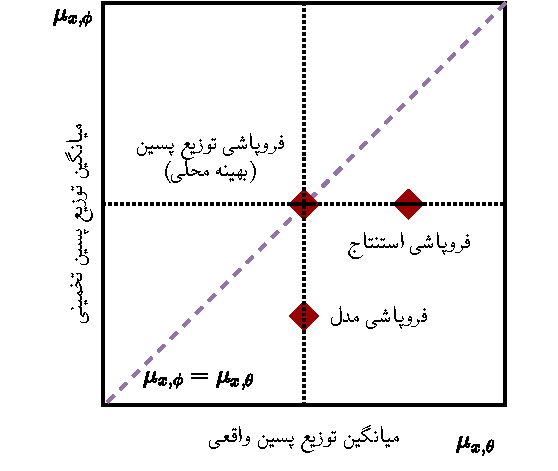
\includegraphics[width=0.5\textwidth]{images/lagging1.pdf}
	\caption
    [نموداری بر فضای میانگین توزیع پسین $(\mu_{x,\phi}, \mu_{x,\theta})$.]
    {
		نموداری بر فضای میانگین توزیع پسین $(\mu_{x,\phi}, \mu_{x,\theta})$. محور افقی میانگین توزیع \posterior{} مدل و محور عمودی میانگین توزیع \posterior{} تخمینی را نشان می‌دهد. خط چین قطری نیز حالتی را نشان می‌دهد که میانگین توزیع \posterior{} مدل (واقعی) با تخمینی یکسان شده است \cite{infovae}.
	}
\end{figure}

از آنجا که میانگین \priordist{} برابر صفر است، بنابراین اگر $\mu_{\bff{x},\phi} = 0$ شود فروپاشی استنتاج و اگر $\mu_{\bff{x},\theta} = 0$ باشد فروپاشی مدل اتفاق افتاده است \cite{infovae}. لازم به ذکر است که بایستی ابعاد $\bff{z}$ به گونه‌ای باشد تا بتوان آن را به صورت کارا محاسبه کرد؛ ازین رو $\bff{z}$ یک عدد یک بعدی در نظر گرفته شده است. محور قطری نیز مربوط به حالتی است که $p_\theta(\bff{z}|\bff{x})$ و $q_\phi(\bff{z}|\bff{x})$ از نظر میانگین بر یکدیگر منطبق بوده و توزیع پسین تخمینی، کار خود را به درستی انجام داده است. مبدا نیز مربوط به حالت بهینه محلیِ فروپاشی \posteriordist{} است؛ این در حالی است که احتمالا نقاط بهینه محلی مطلوب‌تر جایی بر روی محور قطری و در اطراف مبدا خواهند داشت.
نمودار‌های زیر حاصل انجام این آزمایش در روند آموزش است.

\begin{figure}[H]
	\centering
	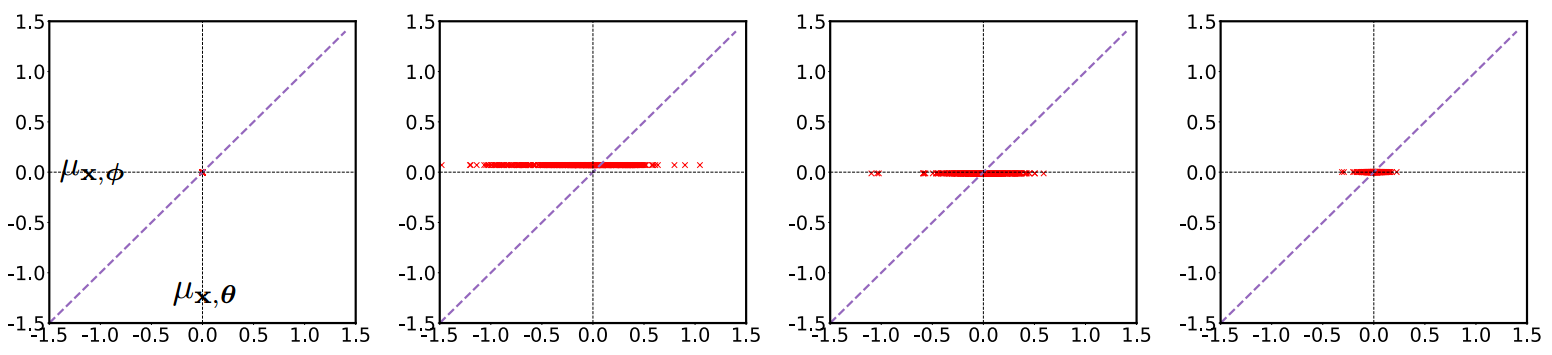
\includegraphics[width=1.\textwidth]{images/lagging2.png}
	\caption
    [مشاهده‌ای از نحوه رخداد حالت فروپاشی استنتاج]
    {
        مشاهده‌ای از نحوه رخداد حالت فروپاشی استنتاج. نمودارهای فوق از تصویر کردن ۵۰۰ نقطه از داده اصلی بر فضای نهان (در ۴ مقطع زمانی. به ترتیب از شکل سمت چپ به راست، گام آموزشی ۰ ام، ۲۰۰ ام، ۲۰۰۰ ام و انتهایی) بدست آمده است. آنچه که در تصویر فوق مشخص است، آن است که در ابتدای آموزش، دو متغیر $\bff{z}$ و $\bff{x}$ از یکدیگر مستقل بوده و در روند آموزش نیز شبکه \encoder{} تخمین صحیحی از \posteriordist{} نداشته و در نتیجه باعث ایجاد حالت فروپاشی استنتاج می‌شود.
	}
\end{figure}
آن طور که از تصاویر برداشت می‌شود به این صورت است که ابتدا نقاط به صورت متمرکز در مبدا جمع شده‌اند اما در ادامه، نقاط در محور افقی گسترده شده‌اند و در انتها مجددا به سمت متمرکز شدن پیش رفته اند. نکته قابل توجه این است که در تمامی این حالات نقاط در محور افقی پراکنده شده‌اند \cite{infovae}. برای توجیه این مشاهده می‌توان از صورت دیگری از رابطه \lr{ELBO} بهره برد. می‌دانیم \lr{ELBO} برابر با عبارت زیر است \cite{vae, vae_lagging}:
\begin{gather}
	\mathcal{L}_{\text{ELBO}}(\bff{x};\theta, \phi) = \log p_\theta(\bff{x}) - {KL}(q_\phi(\bff{Z}|\bff{x})~||~ p_\theta(\bff{Z}|\bff{x}))
\end{gather}
که عبارت اول مربوط به \likelihood{} حاشیه‌ای و عبارت دوم مربوط به فاصله توزیع تخمینی $q_\phi(\bff{z}|\bff{x})$ از توزیع پسین واقعی مدل ($p_\theta(\bff{z}|\bff{x})$) است. واضح است که پارامتر $\phi$ تنها تحت تاثیر عامل \lr{KL} بوده در حالی که پارامتر $\theta$ علاوه بر این، تحت تاثیر عبارت \likelihood{} حاشیه‌ای نیز هست. علاوه بر این تنها عاملی که باعث ایجاد رابطه بین $\bff{x}$ و $\bff{z}$ می‌گردد،
\likelihood{}
است و بخش دوم تنها سعی در نزدیک کردن دو توزیع $p_\theta(\bff{z}|\bff{x})$ و $q_\phi(\bff{z}|\bff{x})$ دارد \cite{infovae}.

حال با نگاه داشتن به رابطه فوق، این پدیده را این طور می‌توان تفسیر نمود که با وجود اینکه ابتدا فضای نهان ساخته شده تقریبا مستقل از فضای داده‌های ورودی است، با پراکنده شدن نقاط به صورت افقی در ادامه روند آموزش، رابطه‌ای بین $\bff{z}$ و $\bff{x}$ تحت مدل $p_\theta(\bff{x})$ در حال شکل‌گیری است؛ اما به دلیل اینکه شبکه \encoder{} به هیچ عنوان تخمین صحیحی از \posteriordist{} واقعی ندارد و همزمان در حال کمینه کردن هر دو قسمت عبارت \lr{ELBO} نسبت به پارامترهای هر دو شبکه‌ی \encoder{} و \decoder{} هستیم، در نتیجه با ادامه آموزش، رابطه بین این دو متغیر به مرور بر اثر غلبه بخش حاوی فاصله \lr{KL} بر بخش \likelihood{} حاشیه‌ای، از دست رفته و سیستم دچار یک بهینه محلی می‌گردد \cite{infovae}.

\subsection{مدل‌های ارائه شده برای رفع مشکل صفر شدن \lr{KL}}
به طور کلی راه حل‌های ارائه شده یا از جنس تغییر معماری ‎\decoder{}‎ و ضعیف کردن قدرت ‎\autoregressive{}‎ آن، تغییر ‎\priordist{}‎ و یا تغییر تابع هزینه هستند.
\\
\subsubsection{استفاده از \cnn{} به جای \lstm{} در \decoder{}}
\begin{figure}[h]
	\centering
	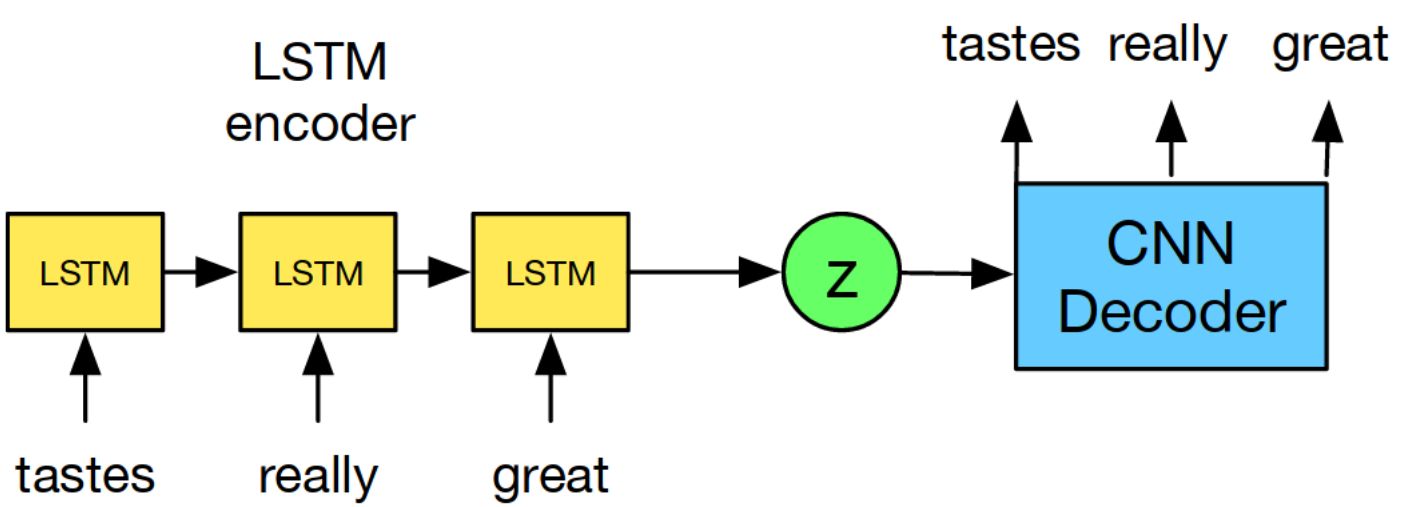
\includegraphics[width=0.5\textwidth]{images/dialated-conv1.png}

	\vspace{0.5cm}

	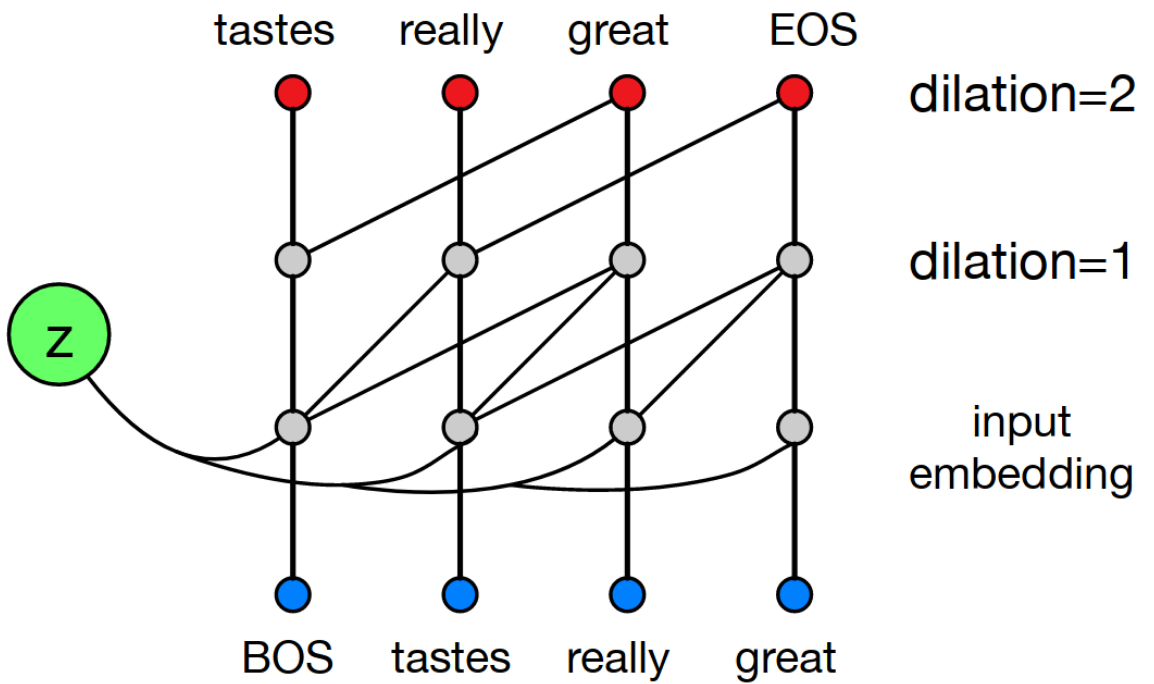
\includegraphics[width=0.5\textwidth]{images/dialated-conv2.png}
	\caption{
		معماری کلی شبکه ارائه شده که از \cnn{}  با کانولوشن‌های \dilated{} در  ‎\decoder{}‎ بهره می‌برد.
	}
	\label{fig:dialted_conv}
\end{figure}
راه حل‌های اولیه بیشتر در حوزه تغییر ساختار ‎\decoder{}‎ هستند. دلیل چنین رویکردی در این بود که می‌توان مشکل را در قدرت زیاد مدل‌های ‎\lstm{} در مدلسازی به صورت ‎\autoregressive{}‎ جست و جو کرد \cite{vae_dialated}؛ چراکه در حوزه تصویر که هر پیکسل مستقل از سایر پیکسل‌ها تولید می‌گردد، چنین پدیده‌ای گزارش نشده است. بنابراین یک راه حل استفاده از مدل‌هایی است که قدرت \autoregressive{} کمتری دارند. برای مثال همان طور که در شکل ‎\ref{fig:dialted_conv}‎ نشان داده شده است، می‌توان ‎\decoder{}‎ را با وام گرفتن از ایده شبکه ‎\lr{PixelCNN}‎ با معماری ‎\cnn{}‎ پیاده‌سازی و جایگزین ‎\lstm{}‎ نمود. به طور دقیق‌تر برای پیشبینی هر پیکسل، پیکسل‌های پیش‌رو پوشانده شده، از فیلتر‌های یک بعدی و اتصالات
\trans{\dilated{}}{Dilated}
در کانولوشن‌ها بهره گرفته شده که در نتیجه
\trans{\receiptivefield{}}{Receiptive field}
در هر لایه نسبت به لایه قبل، افزایش نمایی پیدا کند \cite{vae_dialated}. در واقع با زیاد شدن تعداد لایه‌های با کانولوشن‌های \dilated{}، 
\trans{زمینه}{Context}
 طولانی‌تری در خروجی یک گره از لایه مورد نظر دخیل خواهد شد. برای مثال اگر ضریب انبساط ۲ استفاده گردد، \receiptivefield{}‎ در هر لایه نسبت به لایه قبل تقریبا دو برابر شده و در نتیجه از آنجا که می‌بایست کلمه آخر جمله تابعی از تمام کلمات پیشین باشد،‌ نیاز به $‎\log T$ لایه خواهد بود که $T$ طول بلندترین جمله است. ادعای مقاله بر اساس آزمایش‌های متفاوت بر این است که ساختار \cnn{} بیشتر متکی بر فضای نهان  $Z$ بوده و بنابراین مشکل ذکر شده را مقداری تقلیل می‌دهد. نکته قابل ذکر این است که در این حالت نیز اگر ‎اندازه شبکه بسیار بزرگ شود مجددا مشکل صفر شدن ‎\lr{KL}‎ ظهور پیدا می‌کند \cite{vae_dialated}.

\subsubsection{\aae} \label{sec:aae}
مدل 
\trans{\aae{}}{Adversarial autoencoder}،
نسخه تغییر یافته‌ای از مدل \vae{} است تا بخشی از ضعف‌های آن را بپوشاند. همان طور که قبلا نیز توضیح داده شد، تابع هزینه \vae{} از دو بخش تشکیل شده است. بخش اول مربوط به کمینه کردن خطای بازسازی و بخش دوم مربوط به سوق دادن فضای نهان به توزیع گاوسی نرمال است. مدل \aae{}، با حفظ بخش مربوط به خطای بازسازی، در بخش دوم به جای نزدیک کردن توزیع خروجی ‎\encoder{}‎ به  ‎‎\priordist{‎}‎
($q(\bff{z}|\bff{x}) ‎\leftrightarrow p(\bff{z})$)،
سعی در نزدیک کردن توزیع 
\trans{\marginal{}}{Marginal}
خروجی  ‎\encoder{‎}‎  را  به \priordist{} مورد نظر دارد
($q(z) ‎\leftrightarrow  p(z)$) \cite{aae}.
در واقع توزیع \marginal{} $q(\bff{z})$ به صورت زیر تعریف می‌شود:
\begin{gather}
	q(Z) = \sum_\bff{x} p_{data}(\bff{x}) q(\bff{Z}|\bff{x})
\end{gather}
و هدف نزدیک کردن توزیع $q(\bff{z})$ به $p(\bff{z})$ خواهد بود \cite{aae}. بنابراین در مقایسه با مدل \vae{}، اجازه داده می‌شود تا به جای اینکه خروجی \encoder{} به ازای هر نمونه، مستقل از سایر نمونه‌ها به یک توزیع گاوسی نرمال نزدیک شود، توزیع ‎\marginal{}‎ نمونه‌های داده واقعی در فضای نهان، یک توزیع نرمال گاوسی باشد.
\begin{figure}[H]
	\centering
	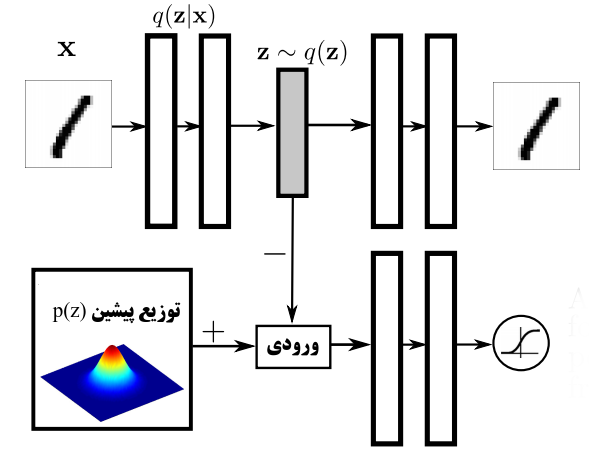
\includegraphics[width=.6\textwidth]{images/aae.png}
	\caption
    [نمایی از مدل  \aae{}.]
    {
		نمایی از مدل  \aae{}. در واقع این مدل، همان مدل \autoencoder{} است که بخش منظم‌ساز مربوط به نزدیک کردن $q(\bff{z})$ به $p(\bff{z})$ به آن افزوده شده است \cite{aae}. برای نزدیک کردن این دو توزیع نیز از رویکرد \gan{} استفاده شده که نمونه‌های \priordist{} نمونه‌های مثبت و نمونه‌های تولید شده توسط \encoder{} نمونه‌های منفی تلقی شده و داده ورودی شبکه \discriminator{} می‌سازند.
	}
	\label{fig:aae}
\end{figure}
گفته شد که بایستی دو توزیع $p(\bff{z})$ و $q(\bff{z})$ به یکدیگر نزدیک شوند. حال بر خلاف آنچه که در مدل \vae{} اتفاق می‌افتاد که بخش $KL$ نیاز به محاسبه به صورت فرم بسته داشت، با وام‌گیری از ایده \gan{}، می‌توان \discriminator ‌ای آموزش داد تا نمونه‌های \priordist{} را از نمونه‌های توزیع \marginal
$q(\bff{z})$
جدا کند. در واقع اگر بخواهیم با ادبیات شبکه‌های تخاصمی معادل‌سازی کنیم، مولد $q(\bff{z})$ و توزیع داده واقعی $p(\bff{z})$ خواهد بود که نمایی از این روش نیز در شکل \ref{fig:aae} آمده است. رابطه تابع هزینه این مدل به شکل زیر است \cite{aae}:
\begin{gather}
	L_{AAE}(\phi, \theta) =
	- \expected_{\bff{x} \sim p_{data}, \bff{z} \sim q_\phi(\bff{Z}|\bff{x})} [\log (D(\bff{z}))]
	+ \expected_{\bff{x} \sim p_{data}, \bff{z} \sim q_\phi(\bff{Z}|\bff{x})}[\log p_\theta(\bff{x}|\bff{z})]\\
	L_{AAE}(D) =
	- \expected_{\bff{z} \sim p(\bff{Z})} [\log D(\bff{z})]
	- \expected_{\bff{x} \sim p_{data},\bff{z} \sim q_\phi(\bff{Z}|\bff{x})} [\log (1 - D(\bff{z}))]
\end{gather}
که $q_\phi(\bff{z}|\bff{x})$ توزیع \encoder{}،
$p_\theta(\bff{x}|\bff{z})$
توزیع \decoder{} و $p(\bff{z})$ توزیع پیشین است. روند بهینه‌سازی به این صورت است که مانند \gan{} از دو بخش تشکیل شده است؛ بخش بهینه‌سازی خطای بازسازی و بخش تخاصمی. در بخش خطای بازسازی، تنها \autoencoder{} به منظور کاهش خطای بازسازی آموزش داده می‌شود و در بخش تخاصمی، ابتدا \discriminator{} به منظور جداسازی نمونه‌های واقعی از مصنوعی و سپس \encoder{} به منظور نزدیک کردن توزیع \marginal{}‎ فضای نهان به \priordist{} آموزش داده می‌شود \cite{aae}.\\
نکته دیگری که می‌توان در نحوه آموزش مدل به آن اشاره نمود این است که کافیست تا بتوانیم از دو توزیع پیشین و حاشیه‌ای \encoder{} نمونه‌برداری کنیم و مانند مدل \vae{}، نیازی به داشتن فرم بسته رابطه بالا نیست که از مزیت‌های این مدل به شمار می‌رود؛ اما از سوی دیگر این مدل بدون پشتوانه نظری و بررسی رابطه آن با \likelihood{} ارائه شد.\\
در مورد نحوه عملکرد ‎\encoder{}‎ چندین گزینه وجود دارد:
\begin{itemize}
	\item \textbf{\deterministic{}:}
	      در اینجا، $q(\bff{z}|\bff{x})$ یک تابع قطعی از $x$ بوده و تنها عامل تصادفی بودن توزیع  $q(\bff{z})$، توزیع داده واقعی $p_{data}‎(\bff{x})$ است \cite{aae}.
	\item \textbf{توزیع \posterior{} گاوسی:}
	      می‌توان خروجی ‎\encoder{}‎ را توزیع گاوسی با ماتریس کوواریانس قطری در نظر گرفت. بنابراین دو عامل تصادفی در $q(\bff{z})$ وجود خواهد داشت؛ توزیع داده اصلی و توزیع خروجی ‎\encoder{}‎ . به منظور آموزش مدل مشکلات مشابه آموزش ‎\vae{}‎ وجود دارد که مجددا می‌توان از ترفند ‎\reparametrization{}‎ بهره برد \cite{aae}.
	\item \textbf{\trans{\uniaprox{}}{Universal approximator} توزیع \posterior{}:}
	      این حالت، کلی‌ترین حالت ممکن برای ‎‎\encoder{}‎ است. ‎\encoder{}‎ به این صورت عمل می‌کند که با گرفتن نویز $‎‎\eta$ (با داشتن توزیع از قبل تعریف شده) و نمونه $\bff{x}$، یک $\bff{z}$ در فضای نهان تولید می‌کند. در واقع ‎\encoder{}‎ یک تابع قطعی از $\bff{x}$ و $‎\eta$ است. مانند حالت قبل، دو عامل تصادفی وجود دارد؛ توزیع داده اصلی و توزیع نویز اولیه. اما بر خلاف مدل قبل، خروجی ‎\encoder{}‎ ، توزیع از پیش تعیین شده‌ای نداشته و با پارامترهای ‎شبکه \encoder{}‎ پارمتری می‌شود. در این حالت $q(\bff{z})$ به شکل زیر خواهد بود:
	      \begin{gather}
		      q(\bff{z}) = \sum_\bff{x} q(\bff{z}|\bff{x}) p_{data}(\bff{x}) = \sum_\bff{x} \sum_\eta p_{data}(\bff{x}) p(\eta)  q(\bff{z}|\bff{x}, \eta)
	      \end{gather}
\end{itemize}
لازم به ذکر است که در دو حالت آخر، ‎با داشتن دو عامل تصادفی، احتمالا توزیع  ‎\marginal{}‎ ‎\encoder{}‎ ، توزیعی با تغییرات  نَرم‌تر خواهد بود \cite{aae}.
\subsubsection{\wae} \label{chap2:wae}
مدل \wae{} که در ادامه معرفی خواهد شد، نسخه عمومی‌تر مدل \aae{}‎ بوده که به لحاظ تئوری نیز بررسی گردیده است.\\
در بخش ‎\ref{sec:aae}‎ توضیح داده شد که تفاوت ‎\aae{}‎ با مدل ‎\vae{}‎، در نحوه اعمال توزیع مورد نظر بر فضای نهان است. با تکیه بر همین نکته، حالت کلی‌تری از ‎\aae{}‎ به نام ‎\wae{}‎ ارائه شد. در واقع همان طور که در شکل ‎‎\ref{fig:wae}‎ مشخص است، در ‎\vae{}‎ توزیع خروجی \encoder{} به ازای هر نمونه به ‎\priordist{}‎ نزدیک می‌شود. در نتیجه این عمل، خروجی \encoder{} به ازای نمونه‌های متفاوت مجبور به داشتن همپوشانی خواهد شد؛ بنابراین بازسازی نمونه‌های داده اصلی از فضای نهان با مشکل مواجه خواهد شد. در مقابل، در ‎\wae{}‎ مقداری دست مدل در نحوه اعمال ‎‎\priordist{}‎ به فضای نهان باز بوده و تنها کافیست توزیع ‎\marginal{}‎ حاکم بر فضای نهان دارای ‎\priordist{}‎ باشد \cite{wae}.\\
\begin{figure}[H]
	\centering
	\begin{subfigure}[b]{0.4\textwidth}
		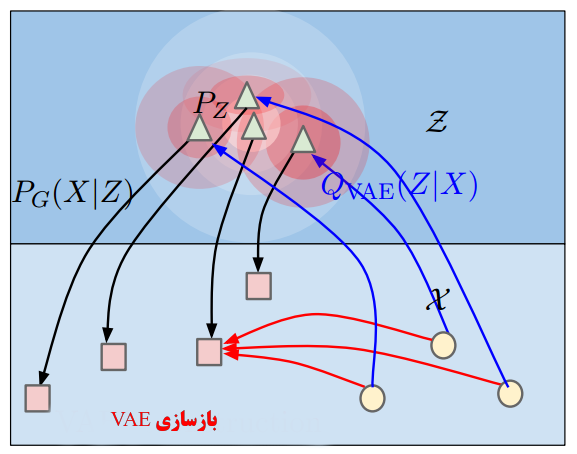
\includegraphics[width=\textwidth]{images/wae1.png}
		\caption{\vae}
		\label{fig:wae-vae}
	\end{subfigure}
	\begin{subfigure}[b]{0.4\textwidth}
		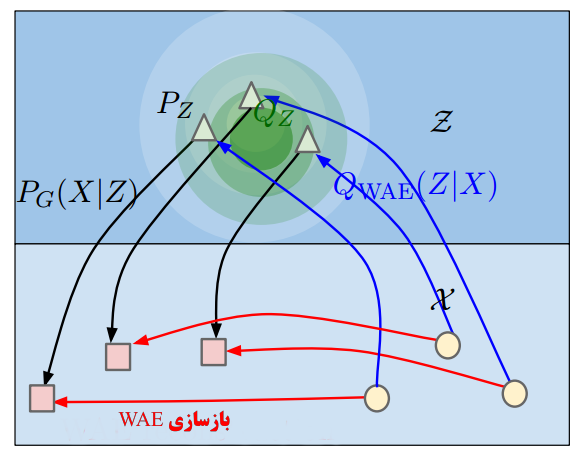
\includegraphics[width=\textwidth]{images/wae2.png}
		\caption{\wae}
		\label{fig:wae-wae}
	\end{subfigure}
	\caption
    [مقایسه نحوه بازسازی در مدل  ‎‎\wae{}‎ با ‎\vae{}‎.]
    {
		مقایسه نحوه بازسازی در مدل  ‎‎\wae{}‎ با ‎\vae{}‎. دوایر قرمز رنگ در فضای نهان مربوط به توزیع (گاوسی) خروجی ‎\encoder{}‎، دوایر سبز رنگ مربوط به توزیع ‎‎\marginal{}‎ خروجی ‎\encoder{}‎ و  دوایر سفید رنگ، متناظر با ‎\priordist{}‎ (گاوسی نرمال) است. همان طور که در شکل ‎\subref{fig:wae-vae}‎ مشخص است، هر ناحیه قرمز سعی در نزدیک شدن به ناحیه سفید رنگ دارد؛ بنابراین به دلیل وجود همپوشانی بین نواحی مختلف قرمز، مشکلاتی در بازسازی پیش خواهد آمد. این در حالیست که در مدل ‎\wae{}‎ ، تمرکز بر اعمال توزیع گاوسی بر توزیع ‎\marginal{}‎ \encoder{}‎‎ است \cite{wae}.
	}
	\label{fig:wae}
\end{figure}
بر خلاف آن که در روش ‎\aae{}‎ اظهار نظری راجع به رابطه تابع هزینه معرفی شده و ‎\likelihood{}‎ مدل ارائه نشد، مدل ‎\wae{}‎ به بررسی این موضوع پرداخته است.
مدل گرافی در نظر گرفته شده برای این روش مانند مدل گرافی ‎\vae{}‎ است. متغیر نهان $\bff{z}$ ای با توزیعی مشخص و ثابت وجود دارد که نمونه $\bff{x}$ از آن بدست خواهد آمد. اگر ‎\priordist{}‎ متغیر نهان را با $p_\bff{Z}(\bff{z})$ و ‎توزیع ‎‎‎\decoder{}‎‎ را با $p_G(\bff{x}|\bff{z})$ نشان دهیم، توزیع ‎\marginal{}‎
$p_G(\bff{x})$
به صورت زیر تعریف می‌شود:
\begin{gather}
	p_G(\bff{X}) = \sum_\bff{z} p_\bff{Z}(\bff{z}) p_G(\bff{X}|\bff{z})
\end{gather}
حال برای اینکه این توزیع را به توزیع $p_{data}‎(\bff{x})$ نزدیک کنیم، از فاصله‌های متعددی می‌توان استفاده نمود \cite{wae}. در اینجا همان طور که از نام مدل بر‌می‌آید، از فاصله ‎‎\trans{‎\wasser{}}{Wasserstein}‎‎‎ بهره برده شده است. اگر فاصله ‎‎\wasser{}‎ با تابع هزینه $c$‎ را با $W_c$ نشان دهیم، اثبات شده است که رابطه $W_c(p_{data}‎, p_G)$ را می‌توان به شرح زیر بازنویسی کرد:
\begin{align}
	\label{eq:wae_constrained}
	W_c(p_{data}, p_G) & = \inf_{\Gamma \in \Pi(p_{data}, \sim p_G)} \expected_{(\bff{x}, \bff{y}) \sim \Gamma} [c(\bff{x}, \bff{y})] \nonumber       \\
	                   & = \inf_{Q: q_z = p_z} \expected_{\bff{x} \sim p_{data}} \expected_{\bff{z} \sim q(\bff{Z}|\bff{x})} [c(\bff{x}, G(\bff{z}))]
\end{align}
که $q_\bff{Z}(\bff{z})$، توزیع ‎\marginal{}‎ فضای نهان است؛ به عبارت دیگر:‌
$q_\bff{Z}(\bff{Z}) = ‎\sum_\bff{x} q(\bff{Z}|\bff{x})p_{data}‎(\bff{x})$
طبق رابطه بالا، به منظور کاهش فاصله ‎\wasser{}‎ بین دو توزیع $p_{Data}‎$ و $p_G$ کافیست توزیع شرطی
$q(\bff{z}|\bff{x})$ای
بیابیم که توزیع ‎\marginal{}‎ آن برابر با توزیع $p_\bff{Z}$ باشد. مشکلی که در رابطه ‎\ref{eq:wae_constrained}‎ وجود دارد این است که مسئله بهینه‌سازی با قید است. به منظور رفع این قید می‌توان آن را به شکل زیر بازنویسی کرد:
\begin{gather}
	V_text{WAE}(q, G) = \inf_{G \in \mathcal{G}, ~ q \in \mathcal{Q}} \expected_{\bff{x} \sim p_{Data}, \bff{z} \sim q(\bff{Z}|\bff{x})} [c(\bff{x}, G(\bff{z}))] + \lambda . D_\bff{Z}(q_\bff{Z}, p_\bff{Z})
\end{gather}
که $‎\mathcal{Q}‎$  و ‎$‎\mathcal{G}$ خانواده توابعی هستند که با شبکه عصبی توانایی مدل کردن آن‌ها را داشته و $D_\bff{Z}(. , .)$ هم می‌تواند هر فاصله‌ای بین دو توزیع $q_\bff{Z}$ و $p_\bff{Z}$ باشد (تنها کافیست بتوان از آن نسبت به پارامترهای شبکه مشتق گرفت)\cite{wae}. لازم به ذکر است که در رابطه بالا، لزومی به تصادفی بودن خروجی ‎\encoder{}‎ نبوده و حالت  ‎\deterministic{}‎ هم می‌تواند داشته باشد.\\
حال اینکه به جای $D_\bff{Z}(. , .)$ از چه معیار یا روشی استفاده گردد، در این مقاله دو گزینه ارائه شده است که بیان خواهند شد:
\begin{itemize}
	\item \textbf{مبتنی بر معماری تخاصمی:}
	      می‌دانیم ‎\gan{}‎‌ها فاصله ‎\lr{JS}‎ را کمینه می‌کنند. به منظور کمینه کردن $D_\bff{Z}(. , .)$ نیز می‌توان از این فاصله بهره برد \cite{wae}. به این صورت که یک شبکه ‎\discriminator{}‎ برای تمیز دادن نمونه‌های ‎\priordist{}‎ از ‎‎نمونه‌های حاصل از خروجی ‎\encoder{}‎ استفاده می‌گردد؛ از سوی دیگر ‎\encoder{}‎ سعی در تولید نمونه‌هایی خواهد داشت که به نمونه‌های ‎\priordist{}‎ نزدیک بوده و ‎\discriminator{}‎ به اشتباه بیفتد. بنابراین اگر \discriminator{} را با $D$ نشان دهیم، توابع هزینه به شکل زیر خواهد بود:
	      \begin{gather}
		      V(q, G)= \inf_{q, G}
		      \expected_{\bff{x} \sim p_{Data}, \bff{z} \sim q(\bff{Z}|\bff{x})} [c(\bff{x}, G(\bff{z}))]
		      - \lambda (\expected_{\bff{x} \sim p_{Data}, \bff{z} \sim q(\bff{Z}|\bff{x})} [\log D(\bff{z})]) \nonumber
		      \\
		      V(D)= \sup_{D}
		      \expected_{\bff{x} \sim p_{Data}, \bff{z} \sim q(\bff{Z}|\bff{x})} [\log (1-D(\bff{z}))]
		      + \expected_{\bff{z} \sim p(\bff{Z})} [\log D(\bff{z})]
	      \end{gather}
	\item \textbf{مبتنی بر فاصله \mmd :}
	      همان طور که در بخش \ref{chap2:divs} توضیح داده شد، اگر تابع کرنل $k$ ویژگی‌های مشخصی را داشته باشد، ‎\mmd{}‎ را به یک متر تبدیل کرده و این امکان را فراهم می‌کند تا از این متر به عنوان تابع هزینه برای کمینه کردن فاصله $p_\bff{Z}$  و $q_\bff{Z}$  بهره برده شود. از آنجا که رابطه بالا به طور مستقیم قابل محاسبه و بهینه‌سازی نیست، از تخمین‌گر نااریب زیر استفاده می‌گردد \cite{wae}. اگر $n$ نمونه از دو توزیع $p_\bff{Z}$  و $q_\bff{Z}$ داشته و به ترتیب با $\bff{z}_i$ و $‎\tilde{\bff{z}}_i$ نشان داده شوند،‌خواهیم داشت:

   \begin{align}
    \mathsf{MMD}_k(\bff{z}{1,2,...,n};\tilde{\bff{z}}_{1,2,...,n}) = & \frac{1}{n(n-1)} \sum_{l \neq j} k(\bff{z}_l, \bff{z}_j) +
    \frac{1}{n(n-1)} \sum_{l \neq j} k(\tilde{\bff{z}}_l, \tilde{\bff{z}}_j)                                               \nonumber          \\
                                                                     & - \frac{1}{n ^ 2} \sum_{l, j} k(\bff{z}_l, \tilde{\bff{z}}_j)
   \end{align}

\end{itemize}‎
بدست آمدن نمونه از توزیع $p_\bff{Z}$ واضح است و برای نمونه‌برداری از توزیع $q_\bff{Z}$ نیز با استفاده از روش
\trans{\ancestral{}}{Ancestral}
ابتدا از توزیع $p_{data}‎$ نمونه‌برداری کرده و سپس از توزیع $q(\bff{z}|\bff{x})$ نمونه‌برداری انجام می‌گیرد.
نکته قابل ذکر این است که قضایای ارائه شده تنها در حالتی که ‎\decoder{}‎ تابعی قطعی باشد صادق هستند؛ البته قضیه مشابهی برای \decoder{} با خروجی تصادفی، اما تنها در حالتی که از تابع هزینه مجذور فاصله استفاده می‌شود، ارائه شده است \cite{wae}.
\subsubsection{
    مدل \autoencoder{} منظم‌شده تخاصمی (\lr{ARAE})
\protect\LTRfootnote{Adversarially Regularized Autoencoder (ARAE)}
} \label{chap2:arae}
این مدل با اینکه قبل از \wae{} منتشر شده است، اما در واقع مربوط به استفاده از \wgan{} و \wae{} در حوزه متن است. در بخش قبل در حالت کلی توضیح داده شد که تابع هزینه \wae{} به صورت زیر است:
\begin{align}
	\mathcal{L}_{\text{WAE}}(q, G) = \expected_{\bff{x} \sim p_{\text{Data}}}\expected_{\bff{z} \sim q(\bff{Z}|\bff{x})} [c(\bff{x}, G(\bff{z}))] + \lambda . D_ \bff{Z}(q_\bff{Z}, p_\bff{Z})
\end{align}
در این مقاله، دو موضوع بررسی شده است. موضوع اول استفاده از تابع هزینه \crossentropy{} به جای $c(.,.)$ بوده و دوم نیز استفاده از \wgan{} به عنوان $D_\bff{Z}(.,.)$ به طوری که مناسب فضای تولید دنباله و متن باشد \cite{wae_text_reg}.
\\
فرض کنید $\mathcal{X} = \mathcal{V}^n$ فضای بردارهای
\trans{\onehot{}}{One-hot}
به طول $|\mathcal{V}|^n$ باشد که $\mathcal{V}$ مجموعه واژگان و $n$ نیز حداکثر طول جملات است (هر بردار متناظر با یک جمله است). همچنین تابع \encoder{} و \decoder{} به ترتیب به صورت
$\text{enc}_\phi: \mathcal{X} \rightarrow \mathcal{Z}$
که تابعی قطعی است و $f_\psi(\bff{Z}) : \mcal{Z} \rightarrow \Delta^{|\mcal{V}|^n - 1}$ تابعی از فضای نهان به
\trans{\simplex{}}{Simplex} $|\mcal{V}|^n - 1$
بعدی (توزیع شرطی بر روی فضای $\mathcal{X}$) است، تعریف شده‌اند. همچنین
\linebreak
$\hat{\bff{x}} = G_\psi(\bff{Z})  = \argmax_{
		\bff{x}} f_\psi(\bff{x}|\bff{Z}) : \mcal{Z} \rightarrow \mcal{X}$
خروجی \decoder{} در حالت آزمون و توزیع $p_\psi(\bff{x}|\bff{z})$ حاصل از آن توزیعی ضربه‌ای به صورت
$p_\psi(\bff{x}|\bff{z}) = \bbm{1}\{\bff{x} = G_\psi(\bff{z})\}$
باشد، تابع هزینه زیر کران بالایی برای فاصله \wasser{} بین $p_\text{Data}(\bff{x})$ و $p_\psi(\bff{x})$ است که
$p_\psi(\bff{x}) = \int_\bff{z} p_Z(\bff{z})p_\psi(\bff{x}|\bff{z})$
:
\begin{align}
	\mathcal{L}_{\text{ARAE}}(q, G) = \inf_{q: q_z = p_z} \expected_{\bff{x} \sim p_{\text{Data}}}\expected_{\bff{z} \sim q(\bff{Z}|\bff{x})} [-\log \bff{x}^T f_\psi(\bff{z})]
\end{align}
در اینجا نیز به مانند بخش آموزش  \wae{} برای رفع قید ذکر شده از نوعی فاصله به نام \wgan{} استفاده می‌شود \cite{wae_text_reg}.
 \wgan{} نیز عضوی از خانواده \gan{} است که رفتار مناسب‌تری هنگام فاصله زیاد مولد از داده اصلی از خود بروز می‌دهد. این روش به شرح زیر است:
در اینجا نیز یک \generator{} و یک \discriminator{} داریم. البته در ادبیات \wgan{} به \discriminator{}،
\trans{\critic{}}{Critic}
گفته می‌شود که وظیفه دارد به نمونه‌های واقعی اعداد بالاتر و به نمونه‌های مصنوعی اعداد پایین‌تری نسبت دهد.
اگر $g_\theta(\bff{\epsilon})$ شبکه‌ای باشد که با گرفتن یک نوفه با توزیع گاوسی نرمال، آن را به نمونه‌ای در فضای نهان تبدیل کند و $f_w(\bff{X})$ یک \critic{} بین نمونه‌های تولید شده توسط مولد ($g$) و داده‌های واقعی باشد، تابع هزینه ذیل استفاده می‌گردد:
\begin{gather}
	\mathcal{L}_\text{WGAN} (g, D)=
	\expected_{\bff{x} \sim p_\text{Data}(\bff{X})} f(\bff{x})
	- \expected_{\bff{x} \sim p_g(\bff{X})} f(\bff{x})
	\\
	\text{\lr{s.t: f is 1-Lipschitz}} \nonumber
\end{gather}
که نسبت به $w$ بیشینه و نسبت به $\theta$ کمینه می‌گردد \cite{wgan}. در واقع تابع هزینه فوق فاصله \wasser{} بین دو توزیع $p_g(\bff{X})$ و $p_\text{Data}(\bff{X})$ است. برای برآوردن شرط \lr{1-Lipschitz} بودن $f$ نیز از روش ساده قطع کردن گرادیان‌های خارج از بازه $[-m, m]$ استفاده شده است \cite{wae_text_reg}.
\\
در این مقاله نیز برای نزدیک کردن فاصله توزیع حاشیه‌ای $q_\bff{Z}$ با $p_\bff{Z}$ از \wgan{} استفاده شده است. در نهایت تابع هزینه‌های این مدل را می‌توان به شکل زیر جمع‌بندی کرد \cite{wae_text_reg}:
\begin{align}
	\min_{\phi, \psi} \mcal{L}_\text{rec}(\phi, \psi) = & \expected_{\bff{x} \sim p_\text{Data}} [- \log f_\phi(\bff{x}|enc_\phi(\bff{x}))] \nonumber
	\\
	\max_{w} \mcal{L}_\text{critic}(w) =                &
	\expected_{\bff{x} \sim p_\text{Data}} [f_w(\text{enc}_\phi(\bff{x}))]
	-\expected_{\bff{z} \sim p_\bff{Z}} [f_w(\bff{z})] \nonumber
	\\
	\min_{\phi} \mcal{L}_\text{enc}(\phi) =                   &
	\expected_{\bff{x} \sim p_\text{Data}} [f_w(\text{enc}_\phi(\bff{x}))]
\end{align}


آنچه که تا به حال توضیح داده شد، روش‌هایی بودند که به نظر موثرتر و پایه‌ای تر به موضوع پرداخته بودند؛ اما مقالات بسیاری در این حوزه ارائه شده است که در اینجا از آن‌ها صرف نظر شده است \cite{vae_decflow, vae_hybrid, vae_multilevel, vae_spherical}.
\iffalse
\subsubsection{دیگر روش‌های جلوگیری از صفر شدن فاصله \lr{KL}}
\fi
نوع دیگری از مدل‌های مولد موجود است که تا به حال چندان نه در حوزه تصویر و به مراتب بیشتر در حوزه متن مورد توجه قرار نگرفته اند. در ادامه به توضیح این دسته نیز پرداخته خواهد شد.
\subsection{\normalizingflownets{}} \label{chap2:flow}
در کنار دو عضو بزرگ از خانواده شبکه‌های مولد مبتنی بر \vae{} و \gan{}، نوع دیگری از شبکه‌ها به نام 
\trans{\normalizingflownets{}}{Normalizing Flow Networks}
 وجود دارند. یکی از مشکلات اساسی ما در این دو نوع \vae{} و \gan{} این است که توانایی محاسبه \likelihood{} به صورت کارا و بدون استفاده از کران‌های پایین و یا بالا وجود ندارد. برای مثال در \vae{} کران پایین \likelihood{} را بیشینه کرده \cite{vae} و در \gan{}‌ها نیز از تابع هزینه دیگری استفاده می‌شود و در مورد رابطه آن با \likelihood{} صحبت شفافی نمی‌توان کرد \cite{gan} (عدم امکان محاسبه \likelihood{} در \gan{} به صورت کلی بیان شد؛ این در حالی است که در حوزه متن امکان محاسبه آن وجود دارد).  بر خلاف این دو دسته، خانواده \normalizingflownets{} توانایی نمونه‌گیری و محاسبه \likelihood{} به صورت کارا را داشته و یا حداقل سعی بر این موضوع دارند \cite{flow_survey}. بنابراین امکان بهینه‌سازی مدل نسبت به تابع هزینه‌ای بر مبنای مقدار دقیق \likelihood{} امکان پذیر است. از سوی دیگر همان طور که تا به اینجا توضیح داده شد، سختی‌ها و نقاط ضعفی از قبیل تنوع نداشتن نمونه‌ها در \gan{} و یا صفر شدن بخش \lr{KL} در \vae{} وجود دارد. این در حالیست که در \normalizingflownets{} با بهینه‌سازی بر اساس \likelihood{} مشکل کم بودن تنوع نمونه‌ها وجود نداشته و یا مشکلات آموزش مانند آنچه ذکر شد، گزارش نشده است. البته این نکته قابل ذکر است که در صورت کم بودن ظرفیت مدل نسبت به توزیع هدف مورد نظر، تابع هزینه مبتنی بر \likelihood{} رفتار \meanseeking{} از خود بروز داده و توزیعی را یاد خواهد گرفت که تمام نقاط را پوشش دهد. بدیهیست که ممکن است برای پوشش دادن تمام نقاط نقاطی نامطلوب را نیز پوشش دهد.
\subsubsection{مفاهیم پایه}
فرض کنید
${\bf{ Z}} \in \mathbb{R}^{D}$
متغیر تصادفی با تابع چگالی احتمال مشخص
$p_{\bf Z}: \mathbb{R}^D$
و $\bf f$ تابعی معکوس پذیر و
${\bf Y} = {\bf f}({\bf Z})$
است. حال با استفاده از قانون تغییر متغیر می‌توان رابطه زیر را نوشت:
\begin{align}  \label{eq:flow_target_dist}
	p_{\bf Y}({\bf y}) = & p_{\bf Z}({\bf g}({\bf y}))
	|\text{det} ~ \text{D} {\bf g}({\bf y})|
	\nonumber                                          \\
	=                    & p_{\bf Z}({\bf g}({\bf y}))
	|\text{det} ~ \text{D} {\bf f}({\bf g}({\bf y}))|^{-1}
\end{align}
که $\bf g$ تابع معکوس $\bf f$ و
$\text{D} {\bf g}({\bf y}) = \frac{\partial {\bf g}}{\partial {\bf y}}$
ماتریس ژاکوبین تابع $\bf g$ و
$\text{D} {\bf f}({\bf z}) = \frac{\partial {\bf f}}{\partial {\bf z}}$
ماتریس ژاکوبین تابع $\bf f$ است. تابع چگالی احتمال حاصل از اعمال تابع $\bf f$ به توزیع پایه را با
$f_*p_{\bf Z}$
نشان خواهیم داد.

در ادبیات مدل‌های مولد، تابع $\bf f$ به عنوان مولد، توزیع پایه
$p_{\bf z}$
را به توزیعی پیچیده‌تر تبدیل می‌کند که به حرکت از توزیع پایه به توزیع نهایی را جهت مولد می‌نامند. به منظور نمونه‌برداری از توزیع نهایی نیز می‌توان از توزیع پایه نمونه برداری کرده و با استفاده از تابع
${\bf y} = {\bf f} ( {\bf z} )$
به نمونه از توزیع نهایی رسید. در جهت مخالف، برای تبدیل توزیع نهایی به توزیع پایه که معمولا توزیع گاوسی نرمال انتخاب می‌شود، از تابع $\bf g$ بهره برده می‌شود. به همین دلیل انتخاب نام جریان نرمال‌کننده بدون هدف نبوده و در واقع جهت مخالف مربوط به تبدیل توزیع پیچیده نهایی به توزیع پایه گاوسی نرمال است \cite{flow_survey}.
\\
به طور کلی اگر تابع $\bf f$ یک تبدیل پیچیده باشد، توانایی تولید هر توزیعی وجود خواهد داشت؛ به عبارت دیگر به ازای هر توزیع هدف
$ p_{\bf Y}({\bf y})$
تابع $\bf f$ای وجود خواهد داشت که
$ p_{\bf Y}({\bf y}) = f_*p_{\bf Z}$.
اما به منظور آموزش و نمونه‌گیری کارا، نیاز است تا این توابع ویژگی‌های خاصی به شرح ذیل داشته باشند \cite{flow_survey}:
\begin{itemize}
	\item
	      معکوس‌پذیر باشند. ممکن است تابع معکوس در جهت نمونه‌گیری و یا جهت نرمال‌ساز به کار برده شود.
	\item
	      به اندازه کافی پیچیده باشند تا بتواند توزیع داده اصلی را مدل کنند.
	\item
	      به لحاظ محاسباتی کارا باشند. برای محاسبه \likelihood{} یک نمونه و نمونه‌گیری نیاز است تا هر دو جهت نمونه‌گیری و نرمال‌ساز به صورت کارا محاسبه شوند. علاوه بر این، طبق رابطه \ref{eq:flow_target_dist} برای محاسبه  \likelihood{} یک نمونه در توزیع نهایی، به محاسبه کارای دترمینان ماتریس ژاکوبین تابع $\bf f$ نیاز است. بنابراین بایستی دترمینان ماتریس ژاکوبین تابع $\bf f$ نیز به صورت کارا محاسبه شود.
\end{itemize}
این خانواده از مدل‌های مولد شامل چندین دسته هستند که در ادامه معرفی خواهند شد.
\subsubsection{جریان‌های
	\trans{\elementwise{}}{Elementwise}}
یک فرم پایه از توابع غیرخطی معکوس‌پذیر را می‌توان از توابع \elementwise{} ساخت. فرض کنید تابع
$h: \mathbb{R} \rightarrow \mathbb{R}$
باشد و معکوس‌پذیر است. اگر
${\bf x} = (x_1, x_2, ..., x_D)^T$
خواهیم داشت:
\begin{gather}
	{\bf f}({\bf x}) = (h(x_1), h(x_2), ..., h(x_D))^T
\end{gather}
برای محاسبه تابع معکوس به تابع $h^{-1}$ نیاز است و از آنجا که ماتریس ژاکوبین آن قطری است پس دترمینان آن ضرب المان‌های روی قطر آن خواهد شد. در واقع چنین تابعی مانند توابع فعال‌سازی مورد استفاده در شبکه‌های عصبی هستند؛ با این تفاوت که این توابع معکوس پذیر نیستند. برای مثال تابع \lr{ReLU} معکوس پذیر نیست اما \lr{ELU} است. به دلیل اینکه این توابع به صورت \elementwise{} عمل می‌کنند، پیچیدگی لازم را ندارند. مدل‌های بعدی سعی در پوشش این ضعف دارند \cite{flow_survey, realnvp, iaf, maf}.
\subsubsection{جریان‌های خطی}
یک تبدیل خطی به طور کلی به شکل زیر تعریف می‌شود:
\begin{align}
	{\bf f}({\bf x}) = {\bf A}{\bf x} + {\bf b}
\end{align}
که $A \in \mathbb{R}^{D \times D}$ و $b \in \mathbb{R}^D$ پارامتر‌های این تبدیل هستند. دترمینان این تبدیل برابر با دترمینان ماتریس ${\bf A}$ بوده و برای معکوس آن نیاز به ${\bf A}^{-1}$ است.
این دو عملیات در حالت کلی با مرتبه زمانی
$O(D^3)$
قابل انجام هستند. اگر توزیع پایه از نوع توزیع‌های نمایی باشد، بعد از اعمال تبدیل فوق در خانواده توزیع‌های نمایی باقی می‌ماند. با این وجود، این دسته یکی از پایه‌های اصلی توابع پیچیده هستند. برای تقلیل زمان محاسبه دترمینان و معکوس تابع، به عناوین مختلف سعی در محدود کردن شکل آن‌ها شده تا این اعمال به صورت کارا انجام پذیرند. برای مثال از پارمتری کردن ${\bf A}$ به صورت پایین مثلثی یا بالا مثلثی بهره برده می‌شود تا دترمینان به صورت بسیار ساده و با ضرب المان‌های روی قطر بدست آید و ماتریس معکوس نیز در $O(D^2)$ محاسبه شود. از آنجا که قدرت این تبدیل وابسته به ترتیب اعمال شده به ابعاد است (هر بعد تابعی از بُعدهای قبل از خود است)، راهکارهای متفاوتی از قبیل تغییر ترتیب به صورت تصادفی و یا یافتن یک ماتریس تبدیل متعامد (حالت کلی‌تر تغییر ترتیب در بعدها) ارائه شده است \cite{flow_survey, glow}.
\subsubsection{جریان‌های
	\trans{\coupling{}}{Coupling}
}
در این گونه از تبدیل‌ها، فضای ورودی به دو زیرفضا تقسیم می‌شود. اگر فضای ورودی را با
$\bff{x} \in \bb{R}^D$
نشان دهیم، دو زیرفضا از آن به صورت
$(\bff{x}^A, \bff{x}^B) \in \bb{R}^d \times \bb{R}^{D - d}$
، تابع معکوس‌پذیر
$\hat{\bff{f}}(.; \theta) : \bb{R}^D \rightarrow \bb{R}^D$
را در نظر بگیرید. یک جریان \coupling{}
$f : \bb{R}^D \rightarrow \bb{R}^D$
را به شکل زیر می‌توان تعریف نمود:
\begin{align}
	\bff{y}^A = & \hat{\bff{f}} (\bff{x}^A; \Theta(\bff{x}^B))
	\nonumber
	\\
	\bff{y}^B = & \bff{x}^B
\end{align}
که $\Theta(\bff{x}^B)$ یک تابع کاملا پیچیده از $\bff{x}^B$ است که به آن
\trans{\conditioner{}}{Conditioner}
، به تابع $\hat{\bff{f}}$ یک لایه \coupling{} و به کل تابع $\bff{f}$ یک جریان \coupling{} گفته می‌شود. نمایی از این جریان در شکل \ref{fig:chap2:flow_coupling} آمده است. معکوس‌پذیری این جریان در گرو معکوس‌پذیری لایه \coupling{} است و در این صورت به شکل زیر محاسبه می‌گردد:
\begin{align}
	\bff{x}^A = & \hat{\bff{f}}^{-1} (\bff{y}^A; \Theta(\bff{y}^B))
	\nonumber
	\\
	\bff{x}^B = & \bff{y}^B
\end{align}
ماتریس ژاکوبین این تابع نیز به صورت یک
\trans{\blocktrimatrix{}}{Block triangular matrix}
است که یکی از بلوک‌های آن ماتریس همانی و دیگری $\text{D}\hat{\bff{f}}$ است. بنابراین دترمینان  تابع $\bff{f}$ دترمینان برابر تابع $\hat{\bff{f}}$ است \cite{flow_survey, realnvp, glow}.

\begin{figure}[H]
	\centering
	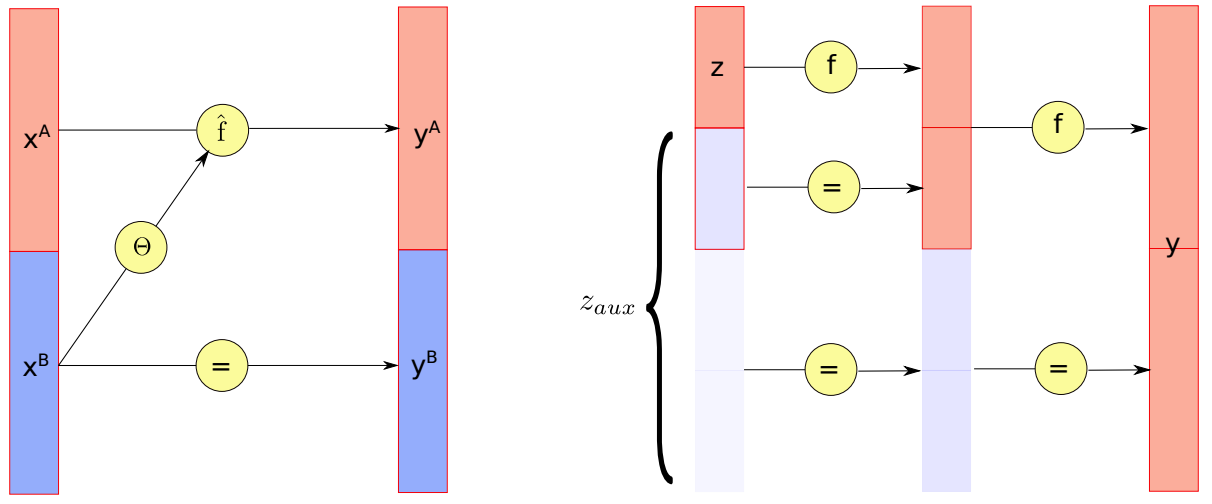
\includegraphics[width=.7\textwidth]{images/flow-survey1.png}
	\caption{
        نمایی از جریان‌های \coupling{}
\cite{flow_survey}	}
\label{fig:chap2:flow_coupling}
\end{figure}

در واقع قدرت اصلی این تابع در میزان پیچیده بودن تابع $\Theta$ است و می‌توان آن را با شبکه عصبی مدل نمود. لازم به ذکر است که این تابع می‌تواند تابعی از $\bff{x}^B$ نباشد و به عنوان اضافه کردن بُعد به کار بسته شود. اما مشکل این تبدیل در نحوه شکستن فضای ورودی به دو فضا است. روش‌های مختلفی نیز از جمله تغییر ترتیب ابعاد به صورت تصادفی برای حل این مشکل ارائه شده است.
\subsubsection{جریان‌های \autoregressive{}}
می‌توان مدل‌های \autoregressive{} را مدل‌هایی از جنس \normalizingflownets{} و نسخه غیر خطی ضرب ماتریس مثلثی در نظر گرفت \cite{flow_survey, iaf, maf}.
\\
مجددا اگر فضای ورودی با
$(x_1, x_2, ..., x_D) = \bff{x} \in \bb{R}^D$
نشان داده شود و
$\hat{\bff{f}} : \bb{R} \rightarrow \bb{R}$
یک تابع معکوس‌پذیر باشد، با داشتن یک ترتیب ثابت بر روی فضای ورودی، تابع \autoregressive{}
$\bff{y} = \bff{f} : \bb{R}^D \rightarrow \bb{R}^D$
به صورت زیر تعریف می‌شود:
\begin{align}
	y_t = \hat{\bff{f}}(x_t; \Theta_t(x_{1:t-1}))
\end{align}
که $t= 2, 3, ..., D$
، $\Theta_t$
یک تابع پیچیده از $\bb{R}^{t-1}$ به فضای پارامترهای تابع $\bff{f}$ و $\Theta_1$ یک تابع ثابت است. در اینجا نیز به $\Theta_t$ یک \conditioner{} گفته می‌شود.
\\
از آنجا که $y_t$ تنها تابعی از $x_{1:t-1}$ است، ماتریس ژاکوبین این تابع نیز مثلثی بوده و بنابراین دترمینان آن از ضرب عناصر قطر آن بدست می‌آید. با داشتن تابع معکوس $\hat{\bff{f}}$، معکوس تابع $\bff{f}$ قابل محاسبه است؛ اما از آنجا که ساختار \autoregressive{} بر روی ابعاد حاکم است، بنابراین  باید هر بعد به صورت ترتیبی از ابعاد قبل به دست آید و درنتیجه نمی‌توان از پتانسیل موازی‌سازی
\trans{\gpu{}}{Graphics Processing Unit}
بهره برد. به منظور موازی‌سازی در جهت نمونه‌گیری، می‌توان از ساختار شبکه‌های \lr{MADE} بهره برد. این شبکه به این صورت است که هر بُعد از آن تنها تابعی از ابعاد قبل از خود است. نمایی از این شبکه در شکل \ref{fig:chap2:made} آمده است \cite{made}.
\begin{figure}[h]
    \centering
    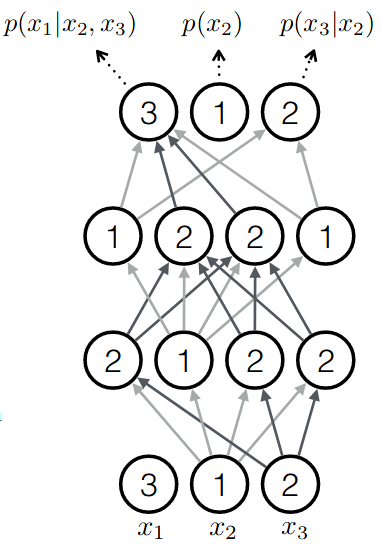
\includegraphics[width=.25\textwidth]{images/made.png}
    \caption{
        نمایی از مدل \lr{MADE}
        \cite{made}.
    }
\label{fig:chap2:made}
\end{figure}
در صورت استفاده از ساختار شبکه \autoencoder{} نقابی برای تخمین توزیع (\lr{MADE})
 \LTRfootnote{Masked Autoencoder for Distribution Estimation (MADE)}
  در $\Theta$، به آن 
جریان \autoregressive{} نقابی (\lr{MAF})
\LTRfootnote{Masked Autoregressive Flow (MAF)}
 گفته می‌شود \cite{maf}.

\begin{figure}[h]
	\centering
	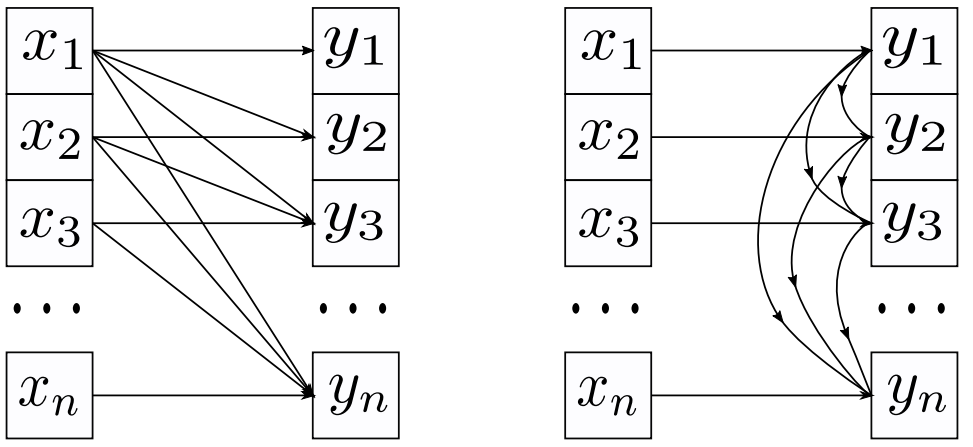
\includegraphics[width=.5\textwidth]{images/flow-survey2.png}
	\caption{
        تفاوت مدل‌های \lr{MAF} و \lr{IAF} به زبان تصویر \cite{iaf, maf, flow_survey}
	}
\label{fig:chap2:mafvsiaf}
\end{figure}

مدل‌سازی تابع \autoregressive{}
$\bff{f}$
را می‌توان به صورت زیر نیز تعریف کرد:
\begin{align}
	y_t = \hat{\bff{f}}(x_t; \Theta_t(y_{1:t-1}))
\end{align}
که در واقع عکس روش \lr{MAF} است. به همین دلیل این روش را جریان \autoregressive{} معکوس (\lr{IAF})
\LTRfootnote{Inverse Autoregressive Flow (IAF)}
 می‌نامند \cite{iaf, flow_survey}. در واقع در \lr{MAF} رفتن از توزیع پایه به توزیع نهایی کُند و رفتن از توزیع نهایی به توزیع پایه سریع است؛ در حالی که \lr{IAF} نمونه‌برداری سریع اما جریان نرمال‌کننده کندی دارد و بایستی بسته به نیاز از آن‌ها بهره برد. تفاوت این مدل در شکل \ref{fig:chap2:mafvsiaf} مشخص است.
نکته قابل ذکر در مورد دسته \autoregressive{}  از \normalizingflownets{} این است که در  بعضی موارد اثبات شده است که این خانواده از توابع، توانایی مدل کردن هر تابعی را داشته و به اصطلاح یک
\trans{\univapprox{}}{Universal approximator}
هستند \cite{flow_survey}.
\subsubsection{لایه‌های \coupling{}}
تا به اینجا در مورد خانواده‌های مختلف \normalizingflownets{} صحبت شد. در تمام آن‌ها از توابع معکوس‌پذیر استفاده شده اما در مورد ساختار آن‌ها توضیحی داده نشد. در این بخش به توضیح تعدادی از توابع معکوس پذیر مورد استفاده پرداخته خواهد شد.
\\
\textbf{لایه
	\coupling{} \trans{\affine{}}{Affine}}:
این لایه‌های خطی، ساده‌ترین و رایج‌ترین لایه‌های مورد استفاده در \normalizingflownets{} هستند. اگر لایه مورد نظر با $\hat{\bff{f}}: \bb{R} \rightarrow \bb{R}$ نشان داده شود، به صورت زیر تعریف می‌شود:
\begin{align}
	\hat{\bff{f}} (x; \theta) = \theta_1 x + \theta_2, \theta_1 \neq 0, \theta_2 \in \bb{R}
\end{align}
این لایه در مدل‌های بسیاری از جمله \cite{iaf, maf} استفاده شده است.
\\
\textbf{لایه \coupling{}
	غیر خطی درجه دو}:
نوع پیشرفته‌تر لایه ذکر شده، نسخه غیرخطی آن‌ها می‌باشد. به این صورت که تابع $\hat{\bff{f}}$ برای مثال به صورت یک تابع درجه ۲ در نظر گرفته می‌شود. به طور واضح چنین تابعی بایستی معکوس‌پذیر باشد؛‌ به همین دلیل از شروط مختلفی برای برآوردن آن استفاده می‌گردد. برای مثال این تابع می‌تواند به صورت زیر تعریف شود:
\begin{align}
	\hat{\bff{f}}(x; \theta) = ax + b + \frac{c}{1 + (dx + h)^2}
\end{align}
تحت شرایطی پارامترهای $\theta=[a,b,c,d]$ یک تابع معکوس پذیر خواهند ساخت و به این هدف، نیاز به محاسبه ریشه تابع فوق که یک تابع درجه ۳ است، خواهد بود \cite{flow_survey}.
\\
\textbf{لایه \coupling{} \spline{}}:
این نام که شاید بیش‌تر در محاسبات عددی شنیده شود، به معنی یک تابع
\trans{تکه‌ای چند جمله‌ای}{Piece-wise polynomial}
است. در واقع اگر $K+1$ نقطه وجود داشته باشد، فواصل بین هر دو نقطه با یک تابع چندجمله‌ای مدل خواهد شد (در واقع $K$ تابع وجود خواهد داشت). حال این توابع باید از نقاط تعیین شده عبور کنند و همچنین در مجموع معکوس‌پذیر باشند. برای محاسبه تابع معکوس نیز پس از تعیین اینکه نقطه مورد نظر مربوط به کدامین تابع از $K$ تابع است، ریشه‌ی معادله مربوطه، جواب خواهد بود \cite{flow_survey}.
\\
\textbf{لایه \coupling{} عصبی}:
نوع کلی‌تری از این لایه‌ها نیز موجود است که با یک شبکه عصبی مدل می‌شوند. به مانند قبل،‌ باید این تابع معکوس‌پذیر باشد؛ برای مثال اگر وزن‌های این تابع همگی مثبت و توابع فعال‌سازی آن یکنوا باشند، این شبکه یک تابع معکوس‌پذیر خواهد بود. در رابطه با این مورد ادعای \univapprox{} نیز وجود دارد \cite{flow_survey}.
\\\\
علاوه بر دسته‌های ذکر شده، دسته‌های دیگری نیز وجود دارند که از حوصله این بحث خارج است. لازم به ذکر است که خانواده \normalizingflownets{} اخیرا بیشتر مورد توجه قرار گرفته و می‌تواند حوزه تحقیقی مورد توجهی باشد.
\subsection{معماری \transformer{}}
معماری‌های معمول استفاده شده در حوزه پردازش متن بیشتر شامل \lstm{} و \cnn{} هستند. اخیرا معماری دیگری به نام \transformer{} مورد توجه قرار گرفت که مخصوص پردازش داده‌های به صورت دنباله بوده و پایه بسیاری از مدل‌های \stateoftheart{} است. در ادامه به معرفی این معماری و اجزای آن پرداخته خواهد شد.
\\
این مدل معماری نیز در گروه مدل‌های
\trans{\seqtoseq{}}{Sequence to sequence}
جای گرفته و از \encoder{} و \decoder{} تشکیل شده است. اگر یک جمله با طول $n$ را با $\bff{x} = (x_1, ..., x_n)$  نشان داده شود، \encoder{} با گرفتن دنباله کلمات $\bff{x}$ (یا هر واحد مورد استفاده دیگر)، این دنباله  را به دنباله بردار‌های پیوسته $\bff{z} = (z_1, ..., z_n)$ تبدیل می‌کند. \decoder{} نیز با گرفتن $\bff{z}$ دنباله کلمات مقصد $\bff{y} = (y_1, ..., y_m)$ خروجی می‌دهد. با اینکه معماری \encoder{} به صورت \autoregressive{} نیست اما \decoder{}، واحدی برای کنترل و ایجاد حالت \autoregressive{} را در خود جای داده است \cite{transformer}.
\begin{figure}[H]
	\centering
	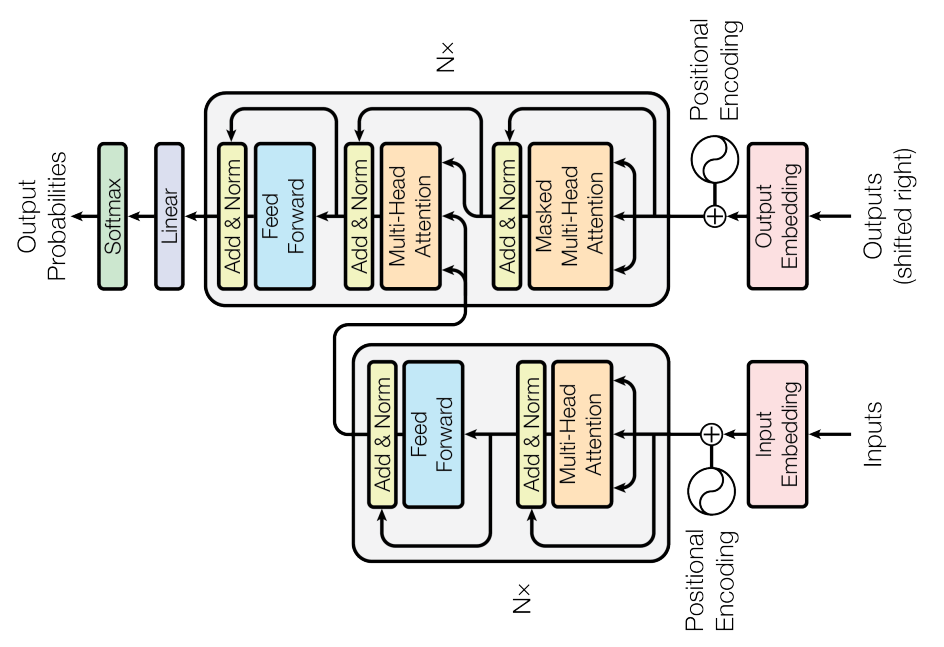
\includegraphics[width=.7\textwidth, angle=-90]{images/attention3.png}
	\caption{
        نمایی از معماری کلی \transformer{} \cite{transformer}}
\end{figure}

\textbf{\encoder{}}:
\encoder{}
از پشته‌ای $N$ لایه یکسان تشکیل شده است. هر لایه شامل دو زیر لایه است. اولین زیر لایه مربوط به نوعی مکانیزم توجه به نام
\trans{\multiheadselfattention{}}{Multi-head Self-attention}
و زیر لایه دوم یک لایه
\trans{\fullyconnected{}}{Fully connected}
است. لازم به ذکر است که در هر زیرلایه از اتصالات
\trans{\residual{}}{Residual}
و
\trans{\layernormalization{}}{Layer normalization}
استفاده شده است\cite{transformer}.
\\
\textbf{\decoder{}}:
\decoder{}
نیز از پشته کردن $N$ لایه تشکیل شده است. هر لایه علاوه بر واحد‌های ذکر شده برای \encoder{}، زیرلایه سومی نیز دارد که شامل
\trans{\multiheadattention{}}{Multi-head Attention}
به خروجی \encoder{} است. در \decoder{} نیز از اتصالات \residual{} و \layernormalization{} استفاده شده است. واحد \multiheadselfattention{} تفاوت کوچکی با واحد مشابه \encoder{} دارد تا در پیشبینی هر کلمه در خروجی، تنها تابعی از کلمات قبل از خود بوده و \autoregressive{} باشد \cite{transformer}.
\\
یک مکانیزم توجه را می‌توان نگاشتی از بردار
\trans{\query{}}{Query}
و یک مجموعه \keyvaluepair{} به یک بردار در نظر گرفت که \query{}، کلیدها و مقدارها همگی بردارند. بردار خروجی از جمع وزن‌دار بردارهای مقدار و هر وزن نسبت داده شده به بردار مقدار، با تابعی از بردار \query{} و کلید بدست می‌آید. در ادامه به شرح دقیق‌تر این مکانیزم پرداخته خواهد شد.
\subsubsection{مکانیزم
	\trans{\dotattention{}}{Scaled Dot-Product Attention}}
این مکانیزم توجه که نام \dotattention{} بر آن نهاده شده است بر روی بردارهای \query{} و کلید $d_k$ بعدی و بردارهای مقدار $d_v$ بعدی اعمال می‌شود. امتیاز هر بردار مقدار با استفاده از ضرب داخلی بردار \query{} در بردار کلید متناظر آن بدست آمده و در نهایت با اعمال تابع \softmax{} بر روی آن وزن مربوطه محاسبه می‌گردد. لازم به ذکر است که برای کنترل واریانس امتیاز هر بردار مقدار، امتیازات قبل از اعمال تابع \softmax{} تقسیم بر $\sqrt{d_k}$ می‌شوند \cite{transformer}.
\begin{figure}[H]
	\centering
	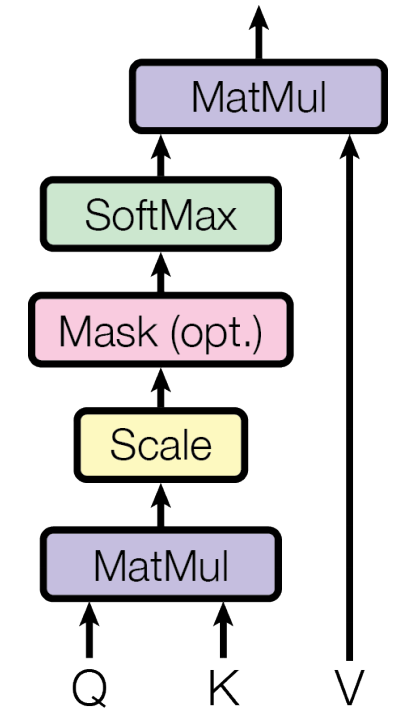
\includegraphics[width=.25
		\textwidth]{images/attention1.png}
	\caption{نمایی از \dotattention{}
    \cite{transformer}.}
\end{figure}
این مکانیزم به صورت زیر می‌توان تعریف کرد:
\begin{align}
	\text{Attention}(Q, K, V) = \text{softmax}(\frac{QK^T}{\sqrt{d_k}})V
\end{align}
که
$Q \in \bb{R}^{n \times d_k}$،
$K \in \bb{R}^{n \times d_k}$ و
$V \in \bb{R}^{n \times d_v}$
به ترتیب بردارهای \query{}، کلید و مقدار هستند.
ویژگی \autoregressive{} در همین نقطه به مدل تزریق می‌شود. اگر امتیاز یک بردار مقدار $-\infty$ شود، وزن نسبت داده شده به این بردار پس از اعمال \softmax{} برابر با صفر خواهد بود؛ بنابراین می‌توان به طور دلخواه تاثیر هر بردار مقدار را با نسبت دادن  امتیاز $-\infty$ به آن، صفر کرد. به ماتریس $n \times n$ بُعدی که ردیف $i$ام آن بیان کننده مکان‌های قابل توجه برای کلمه $i$ام است، ماتریس
\trans{\mask{}}{Mask}
گفته می‌شود (یک برای مکان‌های قابل توجه و $-\infty$ برای مکان‌های غیرقابل توجه) \cite{transformer}.

\subsubsection{مکانیزم \multiheadattention{}}
این امکان وجود دارد که به جای یک بار اعمال تابع توجه بر بردارهای $d_\text{model}$ بُعدی ($d_\text{model}$ اندازه بردار ورودی است)، بردارهای \query{}، کلید و مقدار را با $h$ تبدیل خطی به ترتیب به $h$ فضای مختلف با ابعاد $d_k$، $d_k$ و $d_v$ بُعدی برده و پس از اعمال تابع توجه، نتایجشان را به یکدیگر متصل کرد. لازم به ذکر است که این عملیات‌ها همگی به موازات یکدیگر  قابل انجامند و می‌توان از پتانسیل موازی‌سازی \gpu{} بهره گرفت. در واقع \multiheadattention{} این امکان را به مدل می‌دهد تا با بردن بردارها به فضاهای متفاوت، از چندین فضای مختلف به مکان‌ها و ویژگی‌های مختلف نگاه کرده و در نتیجه به مکان‌های متفاوتی به صورت همزمان توجه کند \cite{transformer}.
\begin{gather}
	\text{MultiHead}(Q, K, V) = \text{Concat}(\text{head}_1, ..., \text{head}_h)W^O \nonumber
	\\
	: \text{head}_i = \text{Attention}(QW_i^Q, KW_i^K, VW_i^V)
\end{gather}
که
$W_i^Q \in \bb{R}^{d_\text{model} \times d_k},
	W_i^K \in \bb{R}^{d_\text{model} \times d_k},
	W_i^V \in \bb{R}^{d_\text{model} \times d_v},
	W^O \in \bb{R}^{hd_v \times d_\text{model}}$
ماتریس‌های تبدیل خطی هستند. لازم به ذکر است که $h \times d_v = d_\text{model}$ است.
\begin{figure}[H]
	\centering
	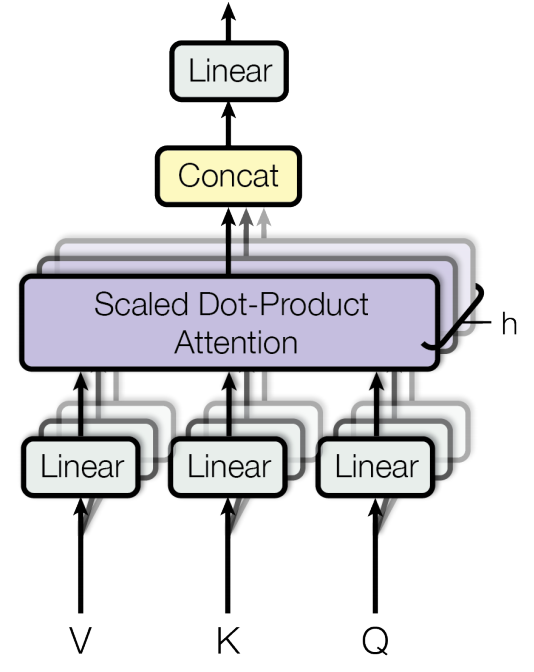
\includegraphics[width=.4
		\textwidth]{images/attention2.png}
	\caption{نمایی از \multiheadattention{}}
\end{figure}
تا به اینجا مکانیزم توجه در \transformer{} توضیح داده شد اما این مکانیزم به چه صورتی و در کجا استفاده شده است؟
\begin{itemize}
	\item
	      در \decoder{} واحد \multiheadattention{} وجود دارد. در اینجا \query{} ها، خروجی لایه قبل \decoder{} و بردارهای مقدار و کلید خروجی‌های \encoder{} هستند. در واقع می‌توان از این مکانیزم تعبیر حافظه نیز داشت \cite{transformer}.
	\item
	      در \encoder{} نیز از \multiheadselfattention{} نام برده شد. \multiheadselfattention{} همان \multiheadattention{} است اگر که بردار \query{}، کلید و مقدار آن یک چیز باشند. بنابراین به ازای هر کلمه، در هر لایه \encoder{}، به تمام خروجی‌های لایه قبل \multiheadselfattention{} زده می‌شود \cite{transformer}.
	\item
	      مجددا در \decoder{} نیز از \multiheadselfattention{} استفاده شده است؛ با این تفاوت که در هر لایه، بردار متناظر با کلمه $i$ با استفاده از \mask{}‌های $-\infty$، تنها تابعی از بردار کلمات قبل‌تر از $i$ خواهد بود \cite{transformer}.
\end{itemize}

\subsubsection{بردار
	\trans{\positionalembedding{}}{Positional Embedding}}
از آنجا که ساختار معرفی شده، خاصیت \recurrence{} ندارد، در هیچ جایی اطلاعاتی راجع به فاصله کلمات نسبت به هم و موقعیتشان در جمله وارد مدل نمی‌شود؛ بنابراین نیاز است تا به نحوی موقعیت کلمات در بردار \embedding{} هر کلمه گنجانده شود که به آن \positionalembedding{} گفته می‌شود. بردار \positionalembedding{}
$PE$
که $d_\text{model}$ بُعدی است، به صورت زیر تعریف شده است \cite{transformer}:
\begin{align}
	PE_{(pos, 2i)} = \sin ( pos / 10000^{2i/d_\text{model}}) \nonumber
	\\
	PE_{(pos, 2i+1)} = \cos ( pos / 10000^{2i/d_\text{model}})
\end{align}
که $pos$ شناسه مکانی مورد نظر است. در مورد نحوه انتخاب روش \encoding{} نیز این طور بیان شده است که
\positionalembedding{}  $i+k$
تابعی خطی از
\positionalembedding{} $i$
است بوده و قابلیت توسعه‌پذیری به جملات با طول‌های بیشتر که در حین آموزش دیده نشده است را ایجاد می‌کند \cite{transformer}. لازم به ذکر است که بردار \positionalembedding{} با بردار \embedding{} کلمه متناظرش جمع خواهد شد.

\section{\condtg}
تا به اینجا به دلیل مشابهت مدل‌های مولد شرطی و غیر شرطی، به معرفی تعدادی از معروف‌ترین مدل‌های مولد غیر شرطی، مشکلات آموزش و راه‌حل‌های رفع آن‌ها پرداخته شد. در این بخش چند مورد مدل مولد شرطی ساده و در ادامه چند مدل شرطی پیچیده‌تر معرفی خواهند شد. در بخش داده را با $\mcal{X} = \{(\bff{x}_n, c_i)\}_{n=1}^N$ نشان می‌دهیم.
\subsection{\rnn{}
     شرطی}
ساده‌ترین رویکردی که در مدل‌های شرطی مورد استفاده قرار می‌گیرد، دخیل کردن شروط مورد نظر به ورودی مولد با ساختار
\trans{\rnn}{Recurrent Neural Network (RNN)}
است. در روش جبر معلم می‌توان شرط را به بردار
\trans{\embedding{}}{Embedding}
و  یا در صورت داشتن بردار نهان، به انتهای بردار نهان ابتدایی مدل مولد متصل نموده و تحویل مدل مولد داد. در واقع مدل مولد به تنهایی بایستی هم ساختار جمله و هم اعمال شروط مورد نظر را به جمله یاد بگیرد.
\subsection{\cvae{}}
نسخه دیگر از \vae{} برای وظایف شرطی موجود است. شیوه تزریق شرط به شبکه به این صورت است که این شروط، هم به \encoder{} و هم به \decoder{} داده خواهد شد \cite{cvae, cvae_semi}. تابع هزینه نیز بسیار شبیه به تابع هزینه \vae{} و کران بالایی برای $\log p_\theta(\bff{x},c)$ است. رابطه آن به صورت زیر است:
\begin{align}
	\mcal{L}_\text{CVAE}(\theta, \phi) = \expected_{(\bff{x},c) \sim \prob_\text{Data}} \Big[
		\expected_{\bff{z} \sim q_\phi(\bff{Z}|\bff{x}, c)} [\log p_\theta(\bff{x}|\bff{z}, c)]
		- KL\big(q_\phi(\bff{Z}|\bff{x},c) ~ || ~ p_\theta(\bff{Z}|c) \big)
		\Big]
\end{align}
که $p_\theta(\bff{Z}|c)$  یک \priordist{} شرطی است.

\subsection{\cgan{}}
در مورد\gan{} نیز شرایطی مشابه \cvae{} حاکم است و شرط به مولد و \discriminator{}، ورودی داده می‌شود \cite{cgan} و رابطه آن به شرح زیر است:
\begin{align}
	\mcal{V}_\text{CGAN}(D, G) =
	\expected_{(\bff{x}, c) \sim \prob_\text{Data}} [\log D(\bff{x}|c)] +
	\expected_{c \sim p(C), \bff{z} \sim N(\bff{0}, \bff{I}),\bff{x} \sim p_G(\bff{X}|z,c)} [\log 1 - D(\bff{x}|c)]
\end{align}
که نسبت به $D$ بیشینه و نسبت به $G$ کمینه می‌گردد.
\begin{figure}[H]
	\centering
	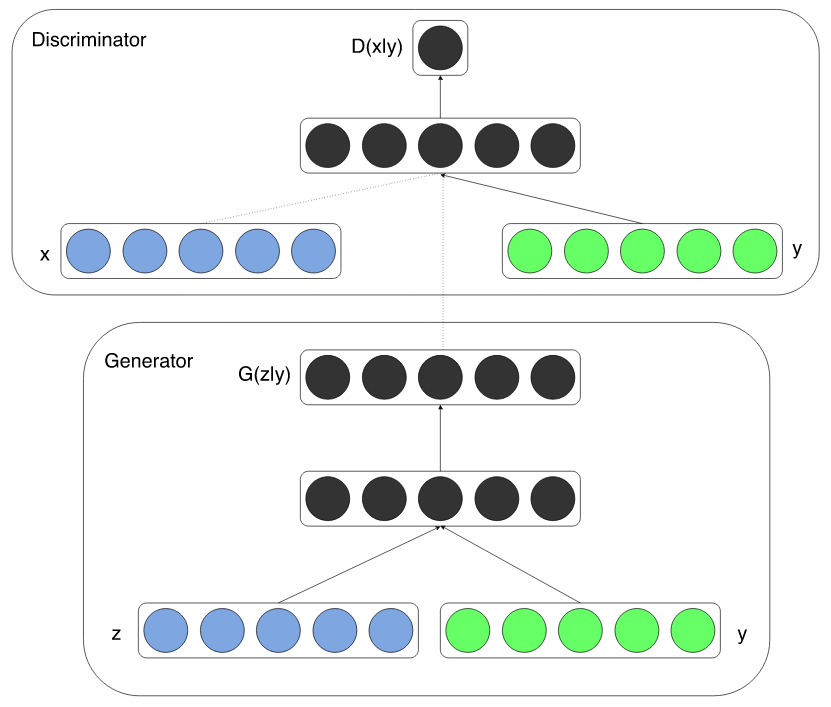
\includegraphics[width=.7\textwidth]{images/cgan.png}
	\caption{نمایی از \cgan{} \cite{cgan}}
    \label{fig:chap2:cgan}
\end{figure}
لازم به ذکر است که مجددا در رابطه فوق مشکل گذر گرادیان وجود دارد و معمولا از روش‌هایی مانند آنچه در بخش \ref{chap2:seqgan} (بر پایه یادگیری تقویتی) است، استفاده می‌شود. نمایی از \cgan{} در شکل \ref{fig:chap2:cgan} آمده است.

\subsection{
    تولید جملاتِ با تمایل، با استفاده از شبکه‌های تخاصمی مخلوط
     (\lr{SentiGAN})\protect\LTRfootnote{Generating Sentimental Texts via Mixture Adversarial Networks (SentiGAN)}
}
در این مدل به منظور تولید جمله با $C$ قطبیت معین، به ازای هر مقدار شرط یک مدل مولد مجزا و یک
\trans{\classifier{}}{Classifier} $C+1$
کلاسه آموزش می‌دهد \cite{sentigan}؛ در این دسته‌بند یک دسته نشانگر داده مصنوعی و سایر دسته‌ها نشان‌گر مقادیر مختلف شرط هستند. در واقع هر مولد سعی در تولید جمله‌ای دارد که از نظر \classifier{} جمله از دسته شرط مرتبط تشخیص داده شده و در مقابل \classifier{} سعی بر نسبت دادن تمام جملات تولید شده توسط مولد‌ها را به دسته $C+1$ام و جملات دادگان اصلی به دسته متناظرشان را دارد و از این جهت همچنان یک \minmaxgame{} در جریان است. اگر
$\{ \bff{x}^n \}_{n=1}^N$
نمونه‌های از توزیع مولد $c$ام با حداکثر طول $T$ باشد، تابع هزینه مدل مولد $c$ام به شرح زیر است:
\begin{align}
	\mcal{L}_\text{SentiGAN}(G_c) = \frac{1}{N}
	\sum_{\bff{x}^n} \sum_{t=1}^{T}
	G_c(\bff{x}^n_t|\bff{x}^n_{1:t-1})
	V_{D_c}(\bff{x}^n_{1:t}, G_c)
\end{align}
که $D_c$ امتیاز \discriminator{} برای دسته $c$ام و تابع $V_{D_c}(., G_c)$ نیز پاداش نسبت داده شده به حرکت $t$ام از مولد $c$ است که برای محاسبه آن مجددا مانند مدل \lr{SeqGAN} (بخش \ref{chap2:seqgan}) از  \montecarlosearch{} برای تخمین پاداش این حرکت استفاده می‌شود. تعریف صوری این پاداش به صورت زیر است:
\begin{align}
	V_{D_c}(\bff{x}_{1:t}, G_c) = \frac{1}{N'} \sum_{n'=1}^{N'} (1 - D_c(\bff{x}_{1:t}, \bff{x}^{n'}_{t+1:T}))
\end{align}
در واقع با ثابت نگه‌داشتن $\bff{x}_{1:t}$،
$N'$
بار جمله را با $G_c$ تکمیل کرده و در نهایت امتیاز \discriminator{} به  $N'$ جمله میانگین گرفته می‌شود. واضح است که برای حرکت آخر (زمانی که $t=T$ است) چنین فرآیندی انجام نمی‌گیرد و از امتیاز \discriminator{} به کل جمله استفاده می‌شود \cite{sentigan}. قابل توجه است که $\mcal{L}_\text{SentiGAN}(G_c)$ با تابع هزینه \wgan{} نیز شبیه بوده، گرچه شرط \lr{K-Lipschitz} بودن برای آن رعایت نشده است
( $G_c(.)V_{D_c}(.)$
به عنوان تابع \critic{} در نظر گرفته شده است).
\\
تابع هزینه دسته‌بند نیز به صورت زیر تعریف می‌شود \cite{sentigan}:
\begin{align}
	\mcal{L}_\text{SentiGAN} (D) =
	- \sum_c \expected_{\bff{x} \sim p_{G_c}} \log D_{C+1} (\bff{x})
	- \expected_{\bff{x} \sim p_\text{Data}(.|c)} \log D_c(\bff{x})
\end{align}

مشخص است که با افزایش تعداد شرط‌ها، این مدل مقیاس‌پذیر نخواهد بود. برای مثلا اگر بخواهیم دو شرط ۳ و ۴ مقداره را مدل کنیم به ۱۲ مدل مولد نیاز است.
\subsection{
    مدل مولد برای تولید متن با شرط‌های مقدار گسسته
(\lr{CSGAN})\protect\LTRfootnote{A Generative Model for Category Text Generation (CSGAN)}}
این مدل نیز شباهت زیادی به مدل \cgan{} دارد. نکته اصلی تفاوت آن با \cgan{} در داشتن سیگنال پاداشی متفاوت است. در \cgan{}،
\discriminator{}
ضمن دریافت جفت جمله و شرط، احتمال نسبت به دسته واقعی یا مصنوعی بودن آن را تعیین می‌کرد؛ از این احتمال به عنوان پاداش در ساختار \reinforce{} برای حل گذر گرادیان استفاده شد. در این مقاله علاوه بر \discriminator{} ذکر شده، یک \classifier{} نیز به کار گرفته شده است و از ترکیب امتیاز واقعی بودن و تعلق جمله به دسته شرط مورد نظر، سیگنال پاداشی غنی‌تری ساخته شده است \cite{csgan}. ضمن حفظ ساختار کلی \cgan{}، دسته‌بند $D_C$ با تابع هزینه ذیل آموزش داده می‌شود:
\begin{align}
	\mcal{L}_\text{CGAN} (D_C) =
	-\expected_{(\bff{x}, c) \sim p_\text{Data}} [\log D_C(c|\bff{x})]
	-\expected_{c \sim p_C, \bff{x} \sim \prob_G(.|c)} [\log D_C(c|\bff{x})]
\end{align}
اگر \discriminator{} را با $D_R$ نشان دهیم، تابع پاداش نیز به شکل زیر تغییر می‌کند:
\begin{align}
	\text{Reward} (\bff{x}, c) =
	\frac{2 D_R(\bff{x},c)D_C(c|\bff{x})}
	{D_R(\bff{x},c) + D_C(c|\bff{x})}
\end{align}
در واقع چه طبیعی نبودن جمله و چه عدم تعلق جمله مورد نظر به دسته شرط مورد نظر باعث جریمه مولد خواهد شد و بالعکس.
\subsection{
    در جهت تولید جملات کنترل شده
(\lr{\towardctg{}})\protect\LTRfootnote{Toward Controlled Text Generation (\towardctg{})}}
شاید این روش یکی از کامل‌ترین روش‌های ارائه شده برای تولید جملات شرطی باشد. بر خلاف مدل‌های ساده قبلی که رابطه بین شروط را در نظر نمی‌گرفتند، این روش علاوه بر تولید جملات صحیح و مرتبط با حالت شرط مورد نظر، سعی در حفظ ساختار و معنای کلی جمله با داشتن حالات مختلف شرط دارد \cite{toward}.
\begin{figure}[h]
	\centering
	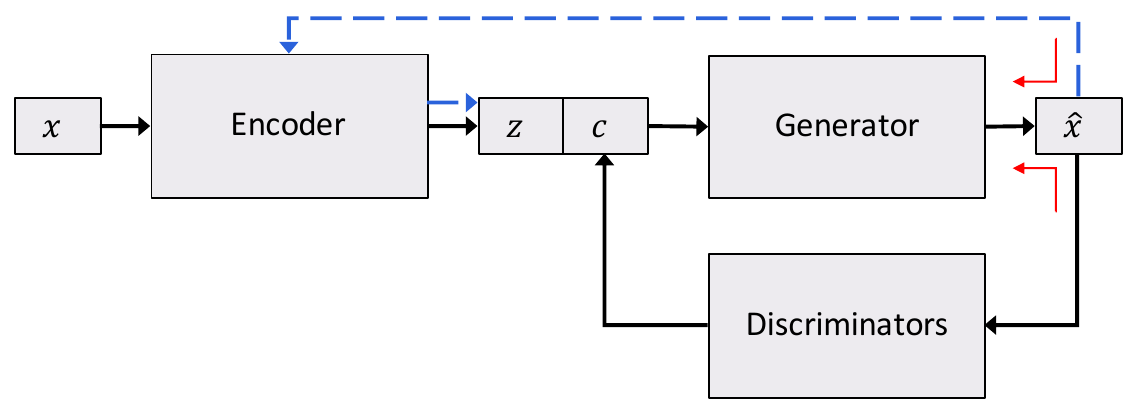
\includegraphics[width=0.5\textwidth]{images/toward1.png}
	\caption
    [نمایی نحوه آموزش مدل \towardctg.]
    {
		نمایی نحوه آموزش مدل \towardctg. خط‌های آبی و سفید جهت حرکت داده و خط‌های قرمز جهت انتفال گرادیان را مشخص می‌کنند \cite{toward}.}
	\label{fig:toward}
\end{figure}
همان‌طور که در شکل \ref{fig:toward} مشخص است، این مدل از ۳ بخش کلی تشکیل شده است؛ یک کدگذار، یک مولد و یک یا چند \discriminator{} که در شکل به جهت سادگی تنها یک نمونه از آن آورده شده است. اگر $c$ نشانگر شرط مورد نظر باشد، وظیفه کدگذار کد کردن جمله ورودی به فضای نهانی است که $c$ در آن ظاهر نشده باشد؛ از سوی دیگر مولد یا در ادبیات مدل‌های پیشین همان کدگشا وظیفه برگرداندن متغیر نهان بدست آمده از کدگذار به جمله اصلی البته با در نظر گرفتن شرط $c$ را داشته و در نهایت \discriminator{} موظف به نظارت بر وجود و رعایت شرط $c$ در جمله تولید شده توسط مولد است. در واقع می‌توان مدل را به صورت یک \vae{} شرطی به همراه یک شبکه \discriminator{} دید که وظیفه نظارت بر شرط مورد نظر را دارد. جهت آموزش این مدل و در نظر گرفتن ویژگی‌های ذکر شده، تابع هزینه از چندین قسمت تشکیل شده است که به اختصار راجع به آن‌ها توضیح داده خواهد شد.\\

\subsubsection*{آموزش کدگذار و مولد}
مطابق با آنچه توضیح داده شد اولین بخش از تابع هزینه مربوط به تابع هزینه شبکه‌های \vae{} شرطی ساده بوده که کنترل‌کننده وظیفه کد کردن و برگرداندن آن به جمله با ویژگی مورد نظر را بر عهده دارد. اگر $E$ کدگذار، $G$ مولد و $D$ \discriminator{} باشد، خواهیم داشت:
\begin{equation}
	\begin{split}
		L_{VAE} (E, G) =& \expected_{\bff{x} \sim p_{data}} [KL (q_E(\bff{Z}|\bff{x}) || N(\textbf{\latin{0}},\textbf{\latin{I}})) - \expected_{\bff{z} \sim q_E(\bff{Z}|\bff{x}), c \sim q_D(C|\bff{x})} [\log p_G(\bff{x}|\bff{z},c)]].
	\end{split}
\end{equation}
از سوی دیگر باید جمله تولیدی توسط مولد حامل ویژگی مورد نظر باشد \cite{toward}. بنابراین تابع هزینه ذیل در نظر گرفته شده است:
\begin{equation}
	\begin{split}
		L_{att, c} (G) =& -\expected_{\bff{z} \sim p(\bff{Z}), c \sim p(C)} [\log q_D(c|G(\bff{z}, c))]
	\end{split}
\end{equation}
که $p(c)$ و $p(\bff{z})$
\trans{توزیع پیشین}{Prior distribution}
تعریف شده روی متغیرهای مربوطه هستند. به عبارت دیگر ابتدا تعدادی نمونه $z$ و $c$ با استفاده از توزیع‌های پیشین تعریف شده ایجاد نموده و سپس مولد بایستی جملاتی را تولید نماید که درست‌نمایی شروط در \discriminator{}‌های مربوطه بیشینه شود.\\
آخرین تابع هزینه‌ای که برای این بخش از مدل در نظر گرفته شده مربوط به حذف وابستگی بین متغیرهای $z$ و $c$ است. به عبارت دیگر مولد بایستی $z$ و $c$ را به جمله‌ای تبدیل نماید که اگر این جمله توسط کدگذار مجددا کد گردد، همان $z$ اولیه بدست آید و جنبه دیگری غیر شروط مورد نظر در جمله تغییر نکرده باشد \cite{toward}. این تابع به شکل زیر تعریف گردیده است:
\begin{equation}
	\begin{split}
		L_{att, z} (G) =& -\expected_{\bff{z} \sim p(\bff{Z}), c \sim p(C)} [\log q_E(\bff{z}|G(\bff{z}, c))].
	\end{split}
\end{equation}
در واقع از سوی دیگر می‌توان کدگذار را به عنوان یک \discriminator{}‌ مشاهده کرد که وظیفه نظارت بر حفظ محتوای جمله غیر از شروط مورد نظر را دارد.
\subsubsection*{آموزش دسته‌بند}
بخش دیگر مربوط به آموزش دسته‌بند می‌باشد؛ اینکه دسته‌بند برچسب شرط هر جمله را به درستی پیش‌بینی کند. لازم به ذکر است که برای هر ویژگی یا شرط، یک دسته‌بند مستقل وجود دارد. برای مثال اگر یک ویژگی زمان فعل و دیگری قطبیت آن باشد، دو دسته‌بند، یکی برای زمان فعل و دیگری برای قطبیت آموزش داده خواهد شد \cite{toward}. بخش اول تابع هزینه شبکه دسته‌بند به شکل ذیل است:
\begin{equation}
	\begin{split}
		L_{s} (D) =& -\expected_{(\bff{x},c) \sim p_{data}} [\log q_D(c|\bff{x})].
	\end{split}
\end{equation}
علاوه بر تابع هزینه فوق، حالتی دیگری نیز که بر اساس نمونه‌برداری از فضای نهان شکل می‌گیرد، وجود دارد و به صورت زیر نوشته می‌شود:
\begin{equation}
	\begin{split}
		L_{u} (D) =& -\expected_{\bff{z} \sim p_\bff{Z}(\bff{Z}), c \sim p(C), \bff{x} \sim p_G(\bff{X}|\bff{z},c)} [\log q_D(c|\bff{x}) + \beta H(q_D(C'|\bff{x}))]
	\end{split}
\end{equation}
که $H(q)$ آنتروپی توزیع $q$ و $\beta$ ضریب تنظیم کننده است که بیشنیه میگردد \cite{toward}؛ علت این موضوع نیز آن است که به دلیل امکان وجود خطا در خروجی \decoder{}، \classifier{} نمیبایستی با قطعیت راجع به برچسب آن اظهار نظر کند؛ در واقع این تابع هزینه به نوعی وظیفه \augmentation{} دارد.
در نهایت توابع هزینه به شکل زیر خواهند بود:
\begin{equation}
	\begin{split}
		L (D) &= L_{s} (D) + \lambda_u L_{u} (D)\\
		L (G) &= L_{VAE} (G) + \lambda_c L_{att, c} (G) + \lambda_z L_{att, z} (G)\\
		L (E) &= L_{VAE} (E)
	\end{split}
\end{equation}
که $(\lambda_s, \lambda_u, \lambda_c , \lambda_z)$ همگی ضرایب تنظیم‌کننده هستند. از دیگر نقاط قوت این مدل باید به دو مورد زیر نیز اشاره نمود:
\renewcommand{\labelitemi}{$\bullet$}
\begin{itemize}
	\item

	      آموزش\trans{نیمه‌نظارتی}{Semi-supervised}:
	      همان‌طور که در روابط و نمای کلی مدل مشخص است، تابع هزینه $L_{VAE}$ نیازی به داده برچسب زده شده نداشته و به شکل \semisupervised{} آموزش می‌بیند. در واقع برای آموزش کل مدل به تعداد زیادی جمله بدون برچسب و تعداد کمتری که در حدود ۳۰۰ جمله که در مقاله ادعا شده است برای برچسب‌زنی نیاز است.
	\item
	      عدم نیاز به داده \trans{جفت برچسب زده شده}{Jointly labeled}:
	      از آنجا که هر شرط مستقل از سایر شروط و برای هر یک، یک دسته‌بند و آموزش مجزا در نظر گرفته شده است، بنابراین نیازی به داده جفت برچسب‌زده شده نیست.
\end{itemize}

در این فصل سعی شد تا در ابتدا فاصله‌های معروف مورد استفاده و سپس مدل‌های زبانی غیر شرطی، به دلیل پایه‌ای بودن این \task{} نسبت به \task{} تولید شرطی، در دو دسته با فضای نهان و بدون فضای نهان، معرفی شوند. در این بین، مشکل عدم توجه به فضای نهان مطرح و راه‌حل‌هایی برای آن ارائه شد. در انتها نیز ضمن شرح معماری نوین \transformer{} و همچنین رویکردِ کمتر مورد توجه \normalizingflownets{}، رویکرد‌های متفاوت آموزش مدل‌های زبانی شرطی توضیح داده شده و مورد بررسی قرار گرفتند.
در فصل بعد ضمن مروری بر ضعف و قوت مدل‌های معرفی شده، مدل پیشنهادی جهت رفع مشکلات ذکر شده و همچنین توانایی در تولید متن به صورت شرطی ارائه خواهد شد.

\chapter{راهکار پیشنهادی}\label{chap3}
\minitoc

\section{مقدمه}
در فصول قبل به بررسی روش‌های پیشین پرداخته شد. این روش‌ها شامل رویکرد‌های مختلفی از جمله مدل‌های مبتنی بر \gan{} و یا \vae{} بودند. در ادامه ضمن مروری بر ویژگی‌های کلی مثبت و منفی این دسته از مدل‌ها سعی بر ارائه مدلی است که مزایای هر دو دسته را در بر داشته باشد.
\\
برای شرطی کردن یک مدل زبانی راهکارهای متفاوتی ارائه شد. در ساده‌ترین حالت می‌توان با وارد کردن شرط به یک شبکه \lr{RNN} به یک مدل شرطی دست یافت. این مدل را از دو جهت می‌توان مورد بررسی قرار داد. اول اینکه به دلیل استفاده از روش \teacherforcing{} در آموزش آن، مدل دارای مشکل \expbias{} است. مشکل دوم که شاید نتوان بر روی آن نام مشکل نهاد، مربوط به عدم داشتن فضای نهان است؛ به عبارت دیگر همان طور که در بخش  \ref{chap1:latent_or_not} توضیح داده شد، این دسته از مدل‌ها غیر از مقدار شرط که در ورودی دریافت می‌کنند، ورودی دیگری ندارند و تنها می‌توان با نمونه‌گیری از توزیع نهایی آن‌ها، به نمونه‌های مورد نظر دست یافت. این در حالیست که اگر مدل دارای فضای نهان می‌بود، این امکان وجود داشت تا با حرکت در اطراف یک نقطه از فضای نهان، خروجی مدل را کنترل کرد.
\\
دسته بعدی از مدل‌ها را می‌توان مدل‌های مبتنی بر \gan{} در نظر گرفت. با وجود اینکه مزیت ویژه این دسته از مدل‌ها در داشتن  نمونه‌های با کیفیت است اما از ضعف‌های حائز اهمیتی همچون \modecollapse{} رنج می‌برند \cite{wgan}. این شرایط در حالیست که به دلیل گسسته بودن فضای جملات، در صورت تمایل به استفاده از \gan{}، در انتقال گرادیان نیز مشکل اساسی وجود خواهد داشت که راه حل‌های آن، یا روش‌های تقریبی بوده و یا واریانس آموزشی بالایی دارند. لازم به ذکر است اکثر مدل‌های مبتنی بر \gan{} در حوزه متن نیز بدون فضای نهان هستند. در صورت داشتن فضای نهان نیز از آنجا که امکان رخداد \modecollapse{} وجود دارد، فضای نهان به تعداد محدودی جمله نگاشت شده و عملا نمی‌توان از آن انتظار تفسیرپذیری چندانی داشت.
\\
دسته آخر نیز مربوط به مدل‌های \vae{} است. این مدل‌ها از این جهت که هم دارای فضای نهان با توزیع مشخص هستند و با کران پایینی از معیار \likelihood{} آموزش داده می‌شوند، برخلاف \gan{} دچار مشکل \modecollapse{} نبوده و می‌توان با نمونه‌برداری از فضای نهان (مانند \gan{}) و \decode{} آن‌ها، به جملات رسید. این مدل‌ها نیز بدون ضعف نیستند. همان طور که در بخش \ref{chap1:latent_ignore} و \ref{chap2:latent_ignore} توضیح داده شد، مشکل اساسی \vae{} در تولید متن، عدم توجه به فضای نهان است. راه حل‌های متعددی برای این مشکل ارائه شده است که بعضی آن را ناشی از مشکلات تابع هزینه می‌دانند. علاوه بر این، به دلیل استفاده از روش ‌\teacherforcing{}، این مدل نیز دچار \expbias{} است. گذشته از این ضعف‌ها مشکلات دیگری نیز برای آموزش دادن شرطی این مدل‌ها گزارش شده است؛ مانند این موضوع که مدل به طور همزمان توانایی داشتن خطای بازسازی کم و هم رعایت شرط ورودی را چندان خوب ندارد. احتمالا به همین دلیل است که در \towardctg{} از یک \classifier{} شرط برای اجبار \decoder{} به رعایت شرط استفاده شده است \cite{toward}.

\subsection{مشاهدات رفتار مدل‌های پیشین}
آنچه توضیح داده شد شرح رفتار مدل‌های مختلف بود. در این بخش دو نمونه از رفتارهای نامطلوب دو دسته \gan{} و \vae{} که در آزمایش با آن‌ها مواجه شدیم، توضیح داده خواهند شد.
\\
مدل اول مدل \towardctg{} است که پایه اصلی آن یک مدل \vae{} می‌باشد. نکته حائز اهمیت این دسته از مدل‌ها میزان تاثیر فضای نهان بر خروجی \decoder{} است. در این مدل، از پارامتر $\tau$ (دما) به منظور کنترل میزان اتکای \decoder{} بر فضای نهان استفاده می‌شود. به طور کلی این پارامتر در تغییر دادن یک توزیع گسسته از حالت یکنواخت به ضربه بسیار کاربردی است. اگر $\bff{o}$ بردار ورودی تابع \softmax{} باشد، پارامتر $\tau{}$ که مقداری بین صفر و یک دارد، به صورت زیر تزریق می‌شود:
\begin{gather}
	\bff{y} = \text{softmax}(\bff{o}/\tau) \\
	\bff{x} \sim p_\bff{y} \nonumber
\end{gather}
منظور از $p_\bff{y}$ توزیع گسسته ایست که احتمالات هر مقدار آن مطابق با $\bff{y}$ است. در رابطه فوق اگر پارامتر $\tau$ دارای مقدار یک باشد، تاثیری بر توزیع $\bff{y}$ نداشته و توزیع به حالت قبلی خود باقی می‌ماند؛ اما هر قدر این پارامتر به سمت صفر پیش رود، توزیع خروجی \softmax{} به سمت توزیع ضربه بر روی بیشینه مقدار بردار $\bff{o}$ پیش خواهد رفت و به عبارت دیگر، \greedydecoding{} خواهد بود. \\
در اینجا نیز می‌توان با تغییر این پارامتر میزان تاثیر فضای نهان بر خروجی \decoder{} را اندازه‌گیری نمود. به طور پیش‌فرض مقدار این پارامتر عددی در حدود ۸.۰ قرار داده شده است. با نمونه‌گیری از فضای نهان و \decode{} کردن آن توسط \decoder{} با پارامتر ذکر شده در دو حالت ۸.۰ و نزدیک به صفر، جملات در جدول 
\ref{table:vae_temp_samples}
بدست آمده‌اند.
	\begin{table}[h!]
        \centering
		\begin{tabular}{|c|c|}
            \hline
			\multirow{9}{5em}{\centering \bf{نمونه‌های با پارامتر دمای 8.0}}
           &\lr{a dream cast of solid female talent who build a seamless ensemble .}\\
           &\lr{ what it lacks in originality it makes up for in intelligence and b - grade}\\
            &\lr{a vivid cinematic portrait .}\\
            &\lr{an impeccable study in perversity .}\\
            &\lr{a gift to anyone who loves both dance and cinema}\\
            &\lr{my advice is to skip the film and pick up the soundtrack .}\\
            &\lr{"a twisty , moody slice of southern gothic ..."}\\
            &\lr{and neither nor suspenseful nor particularly well - drawn in by the center .}\\
            &\lr{it 's basically an overlong episode of tales from the crypt .}\\
            \hline
            \multirow{9}{5em}{\centering \bf{نمونه‌های با پارامتر دمای نزدیک به صفر}}
            &\lr{a film that clearly means to preach exclusively to the converted .}\\
            &\lr{a very average science fiction .}\\
            &\lr{the film 's center will not hold .}\\
            &\lr{ very good film sits the place where a masterpiece of the place .}\\
            &\lr{the movie quickly drags on becoming boring and predictable .}\\
            &\lr{a film that clearly means to preach exclusively to the converted .}\\
            &\lr{a film that clearly means to preach exclusively to the converted .}\\
            &\lr{a film that clearly means to preach exclusively to the converted .}\\
            &\lr{a very average science fiction film .}\\
            \hline
		\end{tabular}
		\caption{خروجی مدل  \towardctg 
            در دو حالت با پارامتر دمای 8.0 و نزدیک به صفر.}
        \label{table:vae_temp_samples}
	\end{table}
واضح است در حالتی که منبع عامل تصادفی تنها از فضای نهان باشد، خروجی مدل یک جمله ثابت خواهد بود. بنابراین این طور می‌توان نتیجه‌گیری نمود که خروجی \decoder{} چندان توسط فضای نهان قابل کنترل نیست و تا حدی مستقل کار می‌کند.
\\
مشابه چنین اتفاقی نیز به لحاظ خروجی مدل در مورد \sentigan{} نیز می‌افتد. در اینجا، به دلیل اینکه فضای نهانی وجود ندارد، بنابراین آزمایش پیش‌تر ذکر شده را نمی‌توان انجام داد. اما مشکل اصلی آموزش \gan{} در کنترل میزان آموزش \generator{} و \discriminator{} و رخداد پدیده \modecollapse{} است. روش معمول این دسته از مدل‌ها به این صورت است که ابتدا یک مرحله، \generator{} با معیار بیشینه \likelihood{} 
\trans{\pretrain{}}{Pretrain}
داده شده و پس از آن با تابع هزینه تخاصمی آموزش داده می‌شود.
 	\begin{table}[h!]
     \centering
     \begin{tabular}{|c|c|}
         \hline
         \multirow{9}{5em}{\centering \bf{ابتدای آموزش تخاصمی}}
         &\lr{a bravura exercise in emptiness .}\\
         &\lr{a movie that is without intent .}\\
         &\lr{a sometimes tedious film .}\\
         &\lr{there 's a reason the studio did n't offer an advance screening .}\\
         &\lr{the movie is a desperate miscalculation .}\\
         &\lr{i liked a lot of the smaller scenes .}\\
         &\lr{a film that is a documentary !}\\
         &\lr{it 's a spectacular performance - ahem , we hope it 's a good bark}\\
         &\lr{visually striking and viscerally repellent .}\\
         \hline
         \multirow{9}{5em}{\centering \bf{پس از رخداد \modecollapse{}}}
         &\lr{a movie that 's about as overbearing and over-the-top as the family it depicts .}\\
         &\lr{a movie that 's about as overbearing and over-the-top as the family it depicts .}\\
         &\lr{a movie that 's about as overbearing and over-the-top as the family it depicts .}\\
         &\lr{a movie that 's about as overbearing and over-the-top as the family it depicts .}\\
         &\lr{a warm , and funny , good-natured treat , slight and and funny , good-natured}\\
         &\lr{a film 's a warm and incendiary movie and good-natured treat of the year 's}\\
         &\lr{a film that clearly means to preach exclusively to the converted .}\\
         &\lr{a film that clearly means to preach exclusively to the converted .}\\
         &\lr{a warm , and funny , good-natured treat , slight and and funny and good-natured}\\
         \hline
     \end{tabular}
     \caption{خروجی مدل \sentigan{}
     در ابتدای آموزش تخاصمی و پس از رخداد \modecollapse{}}
     \label{table:gan_modecollapse_samples}
 \end{table}
 به منظور بررسی موضوع ذکر شده، در حین آموزش دو گام، یکی در ابتدای آموزش تخاصمی و دیگری پس از رخداد \modecollapse{} را انتخاب و از مدل نمونه‌برداری و در جدول 
\ref{table:gan_modecollapse_samples}
گزارش شده است. مجددا شاهد وضعیتی هستیم که تنوع جملات تولیدی توسط مدل بسیار کم شده است. لازم به ذکر است که این موضوع با تغییر میزان آموزش \generator{} و \discriminator{} نیز تغییری نکرد.  از آنجا که به ازای هر شرط یک \generator{} جدا در نظر گرفته است، جملات تولیدی هر \generator{} به تعدادی جمله محدود شده و دو دستگی جملات ذکر شده در حالت \modecollapse{} به این علت است (دادگان آموزشی دارای دو مقدار شرط است).
\\
بنابراین در مجموع هیچ کدام از روش‌های فوق خالی از ضعف نیستند اما از آنجا که هدف در این پروژه تولید جملات به صورت شرطی است، به دو شکل می‌توان مدل گرافی برای فضای نهان در نظر گرفت:
\begin{itemize}
    \item
    فضای نهان $\bff{Z}$ تماما توسط مقدار شرط تعیین می‌گردد (شکل \ref{fig:chap3:latent_pgm_h}).
    \item
    فضای نهان $\bff{Z}$ و شرط از یکدیگر مستقل هستند (شکل \ref{fig:chap3:latent_pgm_d}).
\end{itemize}
که بسته به ماهیت \task{}‌ها و دادگان مختلف، می‌توان از هر کدام استفاده نمود.
\begin{figure}[h]
    \centering
    \begin{subfigure}{0.1\textheight}
        \centering
        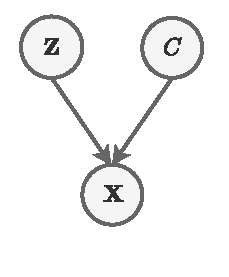
\includegraphics[width=1.\textwidth]{images/pgm_disentangle.pdf}
        \caption{}
        \label{fig:chap3:latent_pgm_d}
    \end{subfigure}
    \hspace{1cm}
    \begin{subfigure}{0.2\textheight}
        \centering
        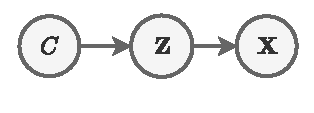
\includegraphics[width=1.\textwidth]{images/pgm_hierarchical.pdf}
        \caption{}
        \label{fig:chap3:latent_pgm_h}
    \end{subfigure}
    \caption{
        دو مدل گرافی متفاوتی که می‌توان برای فضای نهان یک \task{} شرطی در نظر گرفت.
        فضای نهان و شرط مستقل از هم 
        (\subref{fig:chap3:latent_pgm_d})؛
        شرط به طور کامل فضای نهان را تعیین می‌کند
        (\subref{fig:chap3:latent_pgm_h}).
    }
    \label{fig:chap3:latent_pgm}
\end{figure}

\subsection{آموزش \autoencoder{}} \label{chap3:wae_training}
از آنجا که هر دو حالت ذکر شده، مبتنی بر فضای نهان هستند، در طراحی چنین مدلی باید به سوال زیر پاسخ داد:
\begin{itemize}
    \item
    آیا لازم است تا مدلی از خانواده \vae{}  انتخاب شود؟ توزیع حاکم بر فضای نهان چه مزیتی دارد؟
\end{itemize}
برای پاسخ به سوالات فوق لازم است تا هدف و ویژگی‌های مدل‌ها مرور شود. در واقع هدف از داشتن فضای نهان، قابلیت کنترل بر روی فضای نهان و خروجی مدل بود. یکی از این اعمال حرکت بر روی فضای نهان است. حال اگر توزیع مثلا گاوسی بر روی فضای نهان حاکم نباشد، در \autoencoder{}، نقاط به فواصل دوری از هم نگاشت شده و عملا فضا حفره حفره شده و حرکت بر روی آن خروجی مطلوبی نخواهد داشت \cite{infovae}. علاوه بر این جمع کردن فضای نهان جملات در یک توزیع، به دلیل فشرده بودن توزیع هدف، می‌تواند منجر به نزدیک شدن فضای نهان جملات مشابه به یکدیگر شود؛ این در حالیست که همان طور که توضیح داده شد در   \autoencoder{} نقاط نزدیک به هم نگاشت نخواهند شد.
\\
با توجه به دلایل فوق انتخاب یک \autoencoder{} با حاکمیت یک توزیع از پیش تعیین شده بر فضای نهان مبرم به نظر می‌رسد. همان طور که پیشتر اشاره شد \vae{} مشکل عدم توجه به فضای نهان را دارد. به طور کلی راه‌حل‌های ارائه شده برای این مشکل را این طور  می‌توان جمع‌بندی کرد که با وجود اینکه تابع هزینه مورد استفاده در این شبکه‌ها، کران بالایی از منفی لگاریتم \likelihood{} است، اما به طور کلی می‌توان آن را شامل دو بخش بازسازی و منظم‌ساز در نظر گرفت. همان‌طور که در آموزش یک چندجمله‌ای که از تابع منظم‌ساز جمع مجذور وزن‌های تابع استفاده می‌شود و باید میزان توجه و غلبه تابع منظم‌ساز را کنترل کرد، در این مدل‌ها نیز بایستی غلبه بخش \lr{KL} بر بخش بازسازی را کنترل کرد؛ در نتیجه آموزش شبکه سخت خواهد بود. در مقابل یکی از راه‌حل‌های ارائه شده به نام \wae{} با تغییر کوچک تابع هزینه، بخش \lr{KL} را که بین \priordist{} و \posteriordist{} تعریف شده است را به \lr{KL} بین \priordist{} و توزیع حاشیه‌ای \posterior{} تبدیل می‌کند. در نتیجه‌ی این تغییر اثبات می‌کند که تابع هزینه جدید برابر با فاصله \wasser{} بین توزیع داده اصلی و توزیع یادگرفته شده توسط مدل است. توضیح مفصل‌تر این \autoencoder{} و مزیت شهودی آن نسبت به \vae{} در بخش \ref{chap2:wae} آورده شده است.
از سوی دیگر، مقالاتی دیگر به صورت \huristic{}، راه حل‌هایی از جنس اضافه کردن فواصلی بین \priordist{} و توزیع حاشیه‌ای \posterior{} به تابع هزینه \vae{} را ارائه می‌دهند.  بنابراین پاسخ سوال مثبت بوده و از \wae{} استفاده خواهد شد.


\section{شرط به طور کامل فضای نهان را تعیین کند}
در حالتی که فضای نهان به طور کامل توسط مقدار شرط تعیین می‌گردد، اگر بتوان فضای نهانی با قابلیت تفسیرپذیری بالا به وجود آورد، این امکان وجود دارد تا در صورت لزوم با یادگیری هر بخش از فضای نهان به یک شرط خاص دست یافت. به عبارت دیگر با یک بار یادگیری فضای نهان، می‌توان از آن برای یادگیری شروط مختلف بهره برد.
\iffalse
 و از آنجا که معمولا داده برچسب خورده برای هر وظیفه‌ای به تعداد زیاد موجود نیست، بنابراین می‌توان انتظار داشت با توجه به کوچکتر بودن فضای نهان نسبت به فضای ورودی، با داشتن فضای نهان تفسیرپذیر، وظایف مربوط به شروط مختلف را حتی با داده کمتری فرا گرفت.
 \fi
\\
در واقع به صورت غیر مستقیم سعی در یادگیری یک \wae{} شرطی داریم؛ به طوری که \encoder{} و \decoder{} شرطی نبوده اما \priordist{} شرطی باشد. در نتیجه \decoder{} شرطی نبوده و مشکل یادگیری همزمان شرط و محتوا وجود نخواهد داشت. در بهترین حالت باید به دنبال تابع هزینه‌ای بود که \priordist{} شرطی را به توزیع \marginal{} \encoder{} نزدیک کند و بالعکس. به طور کلی دو راه برای این رویکرد وجود خواهد داشت. استفاده از \gan{} و یا \mmd{}. از آنجا که \priordist{} صورت مشخصی ندارد بنابراین استفاده از  \mmd{} چندان معقول نخواهد بود. از سوی دیگر استفاده از \gan{} نیز مشکل \modecollapse{} و سایر مشکلات ذکر شده را در پی دارد. بنابراین راه همواری برای نزدیک کردن دو توزیع به یکدیگر وجود ندارد؛ به طوری که گاهی \priordist{} به توزیع \marginal{} \encoder{} نزدیک شود و گاهی بالعکس. به همین دلیل تنها راه این خواهد بود که پس از اتمام آموزش \autoencoder{} ثابت شده و یک مولد شرطی برای فضای نهان هر مقدار شرط یاد گرفته شود. حال می‌توان برای یادگیری توزیع فضای نهان شرطی از \normalizingflownet{} و تابع هزینه \maxlikelihood{} بهره برد. از آنجا که ممکن است ظرفیت مدل مولد شرطی فضای نهان کمتر از پیچیدگی فضای نهان شروط مختلف باشد، برای کاهش اثر \meanseeking{} تابع هزینه \maxlikelihood{}، سعی می‌شود تا توزیع \marginal{} \encoder{} با توجه به مقادیر شرط جدا‌پذیر بوده و تا حدی اثر پدیده فوق تقلیل پیدا کند.
\\
\begin{figure}[h]
    \centering
    \begin{subfigure}{0.6\textheight}
        \centering
        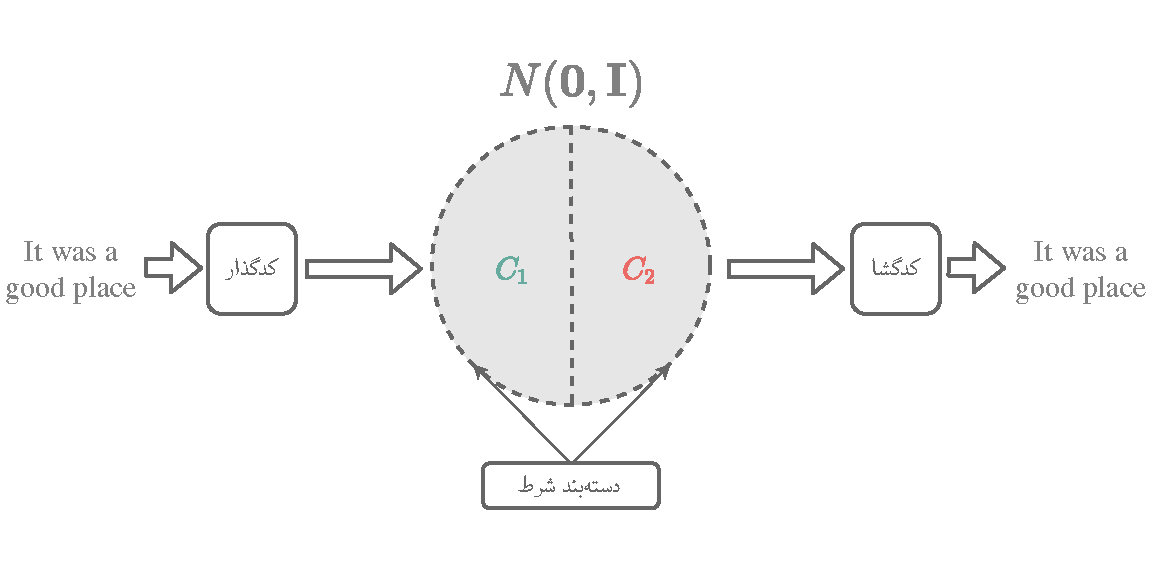
\includegraphics[width=1.\textwidth]{images/propwae.pdf}
        \caption{
            آموزش \autoencoder{} به صورتی که ضمن طبعیت فضای نهان از توزیع گاوسی نرمال، نسبت به مقادیر شرط جدایی پذیر باشد.
        }
        \label{fig:chap4:propwae}
    \end{subfigure}
    \begin{subfigure}{0.5\textheight}
    \centering
    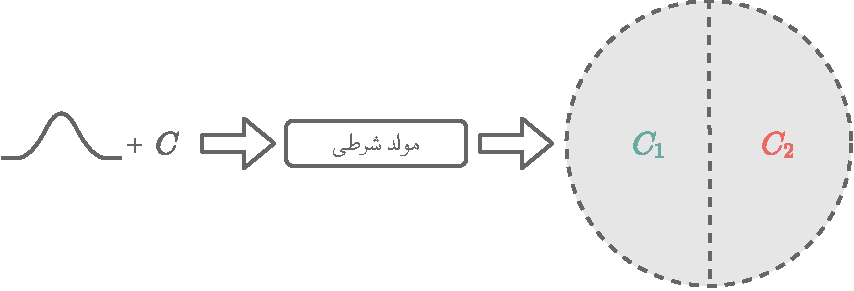
\includegraphics[width=1.\textwidth]{images/propflow.pdf}
    \caption{
پس از مرحله آموزش \autoencoder{} و ساخته شدن فضای نهان مطلوب، یک مدل مولد شرطی فضای نهان آموزش داده خواهد شد. این مدل با دریافت \noise{} و مقدار شرط، برداری در فضای نهان مربوط به مقدار شرط، تولید خواهد نمود.
    }
    \label{fig:chap4:propflow}
\end{subfigure}
\caption{}
    \label{fig:chap4:prop}
\end{figure}
بنابراین همان طور که در شکل \ref{fig:chap4:prop} نشان داده شده است، مدل نهایی از دو بخش کلی تشکیل شده است:
\begin{itemize}
	\item \autoencoder{}:
	      این بخش وظیفه ساختن فضای نهان را بر عهده دارد. در این بخش سعی بر این است تا ضمن یادگیری یک مدل مولد جمله، فضای نهان تفسیرپذیر نسبت به شرط نیز یاد گرفته شود. همان‌طور که ییش‌تر توضیح داده شد، \vae{} در یادگیری همزمان بازسازی جمله و رعایت شرط چندان موفق نیست و حذف عامل شرطی از آموزش \decoder{} می‌تواند باعث رفع این دغدغه گردد.
	\item
	      مولد شرطی: این بخش وظیفه یادگیری یک زیرفضا از فضای نهان که مربوط به شروط مورد نظر است را بر عهده دارد.
\end{itemize}
در ادامه به شرح جزئیات این دو بخش پرداخته خواهد شد.

\subsection{آموزش \wae}
به منظور تبیین صوری تابع هدف، اگر $‎q‎$  و $G$ به ترتیب توابع \encoder{} و \decoder{} باشند، خواهیم داشت:
\begin{gather}
	\mathcal{L}_{\text{WAE}}(q, G) = \expected_{\bff{x} \sim p_{\text{Data}}}\expected_{\bff{z} \sim q(\bff{Z}|\bff{x})} [c(\bff{x}, G(\bff{z}))] + \lambda . D_\bff{Z}(q_\bff{Z}, p_\bff{Z})
\end{gather}
که $c(.,.)$ یک تابع فاصله در فضای ورودی و  $D_Z(. , .)$ هم هر فاصله‌ای بین دو توزیع $q_\bff{Z}$ و $p_\bff{Z}$ است. $q_\bff{Z}$ نیز توزیع حاشیه‌ای حاصل از \encoder{} است؛ به عبارت دیگر:
\begin{gather}
	q_\bff{Z}(\bff{Z}) = \sum_\bff{x} p_{\text{Data}}(\bff{x}) q(\bff{Z}|\bff{x})
\end{gather}
در مقاله اصلی، دو گزینه استفاده از \gan{} و فاصله \mmd{} به عنوان $D_\bff{Z}(.,.)$ پیشنهاد شده است که مجددا به دلیل امکان رخداد \modecollapse{} از \mmd{} بهره برده خواهد شد.
اما به جای $c(.,.)$ نیز بایستی از تابع هزینه مناسبی استفاده نمود. بنابر مقاله توضیح داده شده در بخش \ref{chap2:arae}، اگر تابع $p_\psi$ تابعی از فضای نهان $\bff{Z}$ به فضای احتمال جملات با حداکثر طول مشخص
(فضای خروجی $p_\psi$ یک
\trans{\simplex}{Simplex}
$|V|^m-1$
بعدی است که $m$ حداکثر طول جملات و $|V|$ نیز اندازه واژگان است) و
$G(\bff{Z}) = \argmax_{\bff{x}} p_\psi(\bff{x}|\bff{Z})$
، استفاده از تابع هزینه
$\text{cross-entropy}(p_\psi(\bff{X}|\bff{z}), \bff{x})$
به جای $c(.,.)$،
$\mathcal{L}_{\text{WAE}}(q, G)$
کران بالایی برای فاصله \wasser{} بین توزیع داده‌ها و خروجی مدل است. از آنجا که تابع $G$ به صورت \argmaxphrase{} تعریف شده است، از \greedydecoding{} در \decoder{} که تقریبی از \argmaxphrase{} است استفاده می‌شود.
بنابراین تابع هزینه نهایی به شکل زیر است:
\begin{gather}
	\mathcal{L}_{\text{WAE}}(q, p_\phi) = \expected_{\bff{x} \sim p_{\text{Data}}}\expected_{\bff{z} \sim q(\bff{Z}|\bff{x})} [-\log p_\phi(\bff{x}|\bff{z})] + \lambda_\text{MMD} . \text{MMD}(q_\bff{Z}, p_\bff{Z})
\end{gather}
\iffalse
تا به اینجا همچنان مشکل \expbias{} وجود دارد. همان طور که توضیح داده شد، توزیع $Q_Z$ حاصل از حاشیه‌سازی با $P_\text{Data}$ است و به \priordist{} نزدیک می‌شود. حال اگر $Q_Z$ از حاشیه‌سازی  با هر توزیعی غیر از $P_\text{Data}$ بدست آید، دیگر نزدیک به \priordist{} نخواهد بود. با استفاده از این موضوع می‌توان تابع هزینه دیگری نیز برای تقلیل معضل \expbias{} ارائه داد. اگر خروجی \decoder{} به هر دلیلی از توزیع $P_\text{Data}$ فاصله داشته باشد، توزیع $Q_Z$ حاصل از حاشیه‌سازی با ?? نزدیک به \priordist{} نیست و \decoder{} بایستی سعی در تولید جملاتی داشته باشد تا مجموعه آن‌ها در فضای نهان توزیعی نزدیک به \priordist{} را بسازند. این تابع هزینه را به شکل زیر می‌توان صورت‌بندی کرد:
\begin{gather}
	\mathcal{L}_\text{ExpBias}(G) = \lambda_{e} . D_ Z(Q_Z^G, P_Z)
	\\
	Q_Z^G (z) = \int_{z'} P_Z(z') Q(z|G(z'))
\end{gather}
از آنجا که در روابط هزینه فوق از تابع $\argmax$ استفاده شده است، برای انتقال گرادیان از تقریب \lr{Soft-argmax} بهره برده خواهد شد.  \lr{Soft-argmax} به طور کلی پارامتری به نام $\tau$ دارد که نوع \lr{Straight Through} از به صورت زیر تعریف می‌شود:
\begin{gather}
	\bff{y} = \text{softmax}(\bff{o}/\tau)
	\\
	\bff{u} = \bff{y} - \text{stop-gradient}(\bff{y}) + \text{onehot}(\argmax_{o_i} \bff{o})
\end{gather}
که $\bff{o}$ بردار قبل از اعمال \lr{softmax}
،
$\bff{u}$
بردار خروجی و توابع \lr{onehot} و \lr{stop-gradient} به ترتیب تبدیل‌کننده شاخص به بردار
\trans{\onehot{}}{Onehot}
و قطع‌کننده عبور گرادیان هستند. بنابراین همان طور که از تعریف برداشت می‌شود، در فاز
\trans{\forward{}}{Forward}
هیچ تقریبی وجود ندارد اما در فاز
\trans{\backward{}}{Backward}
گرادیان از طریق تقریب \lr{Soft-argmax}
($\bff{y}$)
منتقل می‌شود.
به منظور آموزش \encoder{} در تفاوت قائل شدن بین توزیع فضای جملات واقعی و فضای جملات تولید شده توسط \decoder{} می‌توان تابع هزینه زیر را نیز در نظر گرفت:
\begin{gather}
	\mathcal{L}_\text{ExpBias}(Q) = -\lambda_{e} . D_ Z(Q_Z^G, P_Z)
\end{gather}
\fi
پیش‌تر بررسی شده است که آموزش مدل فوق، در صورتی که خروجی \encoder{} یک توزیع گاوسی باشد، به سمت صفر کردن واریانس این توزیع و عملا قطعی کردن خروجی \encoder{} و حفره حفره شدن فضای نهان خواهد رفت. برای جلوگیری از این موضوع، از فاصله \lr{KL} بین توزیع گاوسی خروجی \encoder{} و توزیع گاوسی با همان میانگین اما واریانس یک استفاده می‌شود \cite{wasser_text_kl}. به عبارت دیگر تابع هزینه زیر افزوده خواهد شد:
\begin{align}
    \mcal{L}_\text{STD} =& \lambda_\text{STD} ~ \expected_{\bff{x} \sim p_\text{Data}} [
    KL(N(\bff{\mu}_{q(\bff{Z}|\bff{x})}, \bff{\sigma}_{q(\bff{Z}|\bff{x})}) ~ || ~ N(\bff{\mu}_{q(\bff{Z}|\bff{x})}, \bff{I}) ) ] \nonumber
    \\
    =& \lambda_\text{STD} ~ \expected_{\bff{x} \sim p_\text{Data}} [ 
    -\log \bff{\sigma}_{q(\bff{Z}|\bff{x})} + \frac{1}{2} \bff{\sigma}_{q(\bff{Z}|\bff{x})}^2 ] + \text{const}
\end{align}
از آنجا که انتظار دسته شدن جملات با توجه به مقدار شرط در فضای نهان، شاید انتظار بالایی باشد، از یک \classifier{} خطی شرط در فضای نهان استفاده خواهد شد تا \encoder{} جملات را به نحوی \encode{} کند تا \classifier{} بتواند آن‌ها را دسته‌بندی کند. بنابراین اگر \classifier{} را با $q_L(c|\bff{z})$ نشان دهیم، تابع هزینه آموزش \classifier{} به شرح زیر است.
\begin{align}
    \mcal{L}_\text{CLS} (q_L) = -\expected_{(\bff{x}, c) \sim p_\text{Data}(\bff{X},C) , \bff{z} \sim q(\bff{Z}|\bff{x})} \log q_L(c | \bff{z})
\end{align}
از سوی دیگر تابع هزینه زیر نیز به تابع هزینه \encoder{} اضافه خواهد شد:
\begin{align}
\mcal{L}_\text{CLS} (q) = - \lambda_\text{CLS} ~ \expected_{(\bff{x}, c) \sim p_\text{Data}(\bff{X},C) , \bff{z} \sim q(\bff{Z}|\bff{x})} \log q_L(c | \bff{z})
\end{align}
که همان تابع هزینه \classifier{} است و \encoder{} را به \encode{} جملات در فضاهای نسبتا مجزایی با توجه به مقدار شرط سوق خواهد داد.

\subsection{آموزش مولد شرطی}
تا به اینجا در مورد نحوه ساختن یک مدل مولد غیر شرطی اما با فضای نهان مناسب صحبت شد. حال با داشتن فضای نهان بایستی مدل مولد شرطی را آموزش داد تا با گرفتن مقدار شرط، توزیعی بر روی فضای نهان دارای شرط مورد نظر بسازد.
\\
از آنجا که فضای نهان، یک فضای پیوسته است، بنابراین بایستی کمی در مورد نحوه انتخاب مدل مولد و روش آموزش آن تامل کرد. همان‌طور که پیشتر توضیح داده شد، موفق‌ترین مدل‌های مولد، \gan{} و \vae{} هستند. در مورد \gan{} که مشکل \modecollapse{} وجود دارد و در مورد \vae{} نیز از آنجا که فضای ورودی آن فضای نهان جملات است، بایستی برای این فضا، فضای نهان دیگری را بسازد. بنابراین این روش‌ها چندان معقول نیستند. در کنار این روش‌ها رویکرد دیگری نیز وجود دارد که چندان به آن توجه نمی‌شود. یادگیری مدل مولد بر پایه بیشینه کردن مستقیم \likelihood{}. از آنجا که در حال صحبت از فضای پیوسته هستیم، بنابراین بایستی از توزیع‌های پارامتری از پیش تعریف شده مانند گاوسی و یا در بهترین حالت از
\trans{\gaussianmix{}}{Gaussian mixture}
استفاده کرد. از آنجا که فرضی بر توزیع فضای نهان یک شرط خاص نداریم، بنابراین به کار بستن چنین مدل‌هایی چندان معقول به نظر نمی‌رسد. همان طور که در بخش \ref{chap2:flow}‌ توضیح داده شد، نوع دیگری از خانواده‌های مولد وجود دارند که هم امکان محاسبه \likelihood{} در خروجی را دارند و هم فرم مشخصی مانند توزیع گاوسی ندارند. به این دسته از شبکه‌ها \normalizingflownets{} می‌گویند. توضیحات مفصلی در رابطه با معرفی این مدل‌ها در بخش \ref{chap2:flow} ارائه شده است و در اینجا صرف نظر می‌شود.
\\
فرض کنید مدل مولد شرطی را با $p_F(\bff{z}|c)$ که یک شبکه از خانواده \normalizingflownets{} است، نشان داده و مجموعه دادگان آموزشی
$\mathcal{X}_C = \{(\bff{x}_i, c_i)\}_{i=1}^{N}$
باشد. اگر
\begin{gather}
	q(\bff{Z}, \bff{X}|c) = p_\text{Data}(\bff{X}|c) q(\bff{Z}|\bff{X})
	\\
	q(\bff{Z}|c) = \sum_\bff{x} q(\bff{Z}, \bff{x}|c)
    = \sum_\bff{x} p_\text{Data}(\bff{x}|c) q(\bff{Z}|\bff{x})
\end{gather}
خواهیم داشت:
\begin{align}
	\mathcal{L}_c (F) = & KL\big(q(\bff{Z}|c) ~ || ~ p_F(\bff{Z}|c)\big) \nonumber                                          \\
	=                   & \int_\bff{z} q(\bff{z}|c) \log \frac{q(\bff{z}|c)}{p_F(\bff{z}|c) \nonumber}                                  \\
	=                   & -\int_\bff{z} q(\bff{z}|c) \log p_F(\bff{z}|c) + \text{const} \nonumber                                 \\
	=                   & -\int_\bff{z} \sum_\bff{x} p_\text{Data}(\bff{x}|c) q(\bff{z}|\bff{x}) \log p_F(\bff{z}|c) + \text{const} \nonumber       \\
	\Rightarrow
	\mathcal{L}_c (F) = & - \expected_{\bff{x} \sim P_\text{Data}(\bff{X}|c), \bff{z} \sim q(\bff{Z}|\bff{x})} [\log p_F(\bff{z}|c)] + \text{const}
\end{align}
رویکرد‌های متفاوتی نیز برای مدل کردن تابع $F$ وجود دارد؛ اما  همان طور که پیشتر توضیح داده شد، مدل‌های \autoregressive{} از این خانواده به مراتب توانایی مدل‌سازی بیشتری دارند و نقطه ضعف آن‌ها در عدم امکان موازی‌سازی بر روی بُعد است؛ اما از آنجا که ابعاد فضای نهان کوچک است، این نکته چندان مشکل‌ساز نیست. دو نوع ساده از این خانواده \lr{MAF} و  \lr{IAF} است. به دلیل آنکه \lr{IAF} و \lr{MAF} توابع معکوس یکدیگر هستند، \lr{MAF} در ادامه توضیح داده خواهد شد.
\\
اگر تابع $F(\bff{Z}_0, c)$ را به صورت
 $F = F_L \circ F_{L-1} \circ ... \circ F_1 (\bff{Z}_0, c)$
 باشد که $F_l$ یک لایه از نوع \lr{MAF} بوده، خروجی لایه $l$ ام را با $\bff{Z}_l \in \bb{R}^D$ نشان داده و $\bff{Z}_0$ نمونه‌ای از توزیع پایه  $p_{\bff{Z}_0}$ با قابلیت محاسبه کارای احتمال یک نمونه و همچنین نمونه‌برداری باشد (در اینجا توزیع گاوسی نرمال)، بُعد $i$امِ لایه $l+1$ام به صورت زیر تعریف می‌شود:
\begin{align}
	\bff{Z}^i_{l+1, c} = & \bff{Z}^i_{l, c} * \Theta^{i}_{l,1}(\bff{Z}^{1:i-1}_{l+1, c}, c) + \Theta^{i}_{l,2}(\bff{Z}^{1:i-1}_{l+1, c}, c)
\end{align}
و تابع معکوس نیز می‌تواند به صورت برداری به شرح زیر نوشته شود:
\begin{align}
	\bff{Z}_{l-1, c} =  & F_{l}^{-1}(\bff{Z}_{l,c},c) \nonumber
	\\
	\bff{ Z}_{l-1, c} = &
	\frac{\bff{ Z}_{l,c} - \Theta_{l,2}(\bff{Z}_{l,c}, c)}
	{\Theta_{l,1}(\bff{Z}_{l, c}, c)}
\end{align}
که $\Theta_{l,1}$ و $\Theta_{l,2}$ نیز توابعی هستند که با شبکه عصبی مدل می‌شوند؛ تنها محدودیت این شبکه‌ها در این است که بُعد $i$ام آن تنها باید تابعی از ابعاد $1$ تا $i-1$ باشد. به این هدف، از معماری \lr{MADE} در $\Theta_{l,1}$ و $\Theta_{l,2}$ استفاده می‌شود.
\\
از آنجا که هر بُعد بر حسب بعدهای قبل از خود است، بنابراین ماتریس ژاکوبین نیز مثلثی بوده و دترمینان آن برابر با حاصل‌ضرب اعضای قطر آن است.
\begin{align}
	\Big[ \frac{\partial F_{l+1}}{\partial \bff{Z}_{l,c}} \Big]_{i,i} = \Theta^{i}_{l,1}(\bff{Z}^{1:i-1}_{l+1,c}, c) \nonumber
	\\
	\text{det}\Big[ \frac{\partial F_{l+1}}{\partial\bff{Z}_{l,c}} \Big] = \prod_{i=1}^D \Theta^{i}_{l,1}(Z^{1:i-1}_{l+1, c}, c)
\end{align}
بنابراین \likelihood{} نقطه $\bff{z}_L$ به طوری که 
$\bff{z}_0 = F^{-1}(\bff{z}_L, c)$
 نیز طبق رابطه \ref{eq:flow_target_dist} به صورت زیر محاسبه می‌شود:
\begin{align}
	\log p_F(\bff{z}_L|c) = & \log p_{\bff{Z}_0}(\bff{z}_0) - \sum_{l=1}^L \log (\text{det}[    \frac{\partial F_{l+1}}{\partial \bff{z}_{l,c}}     ]) \nonumber
	\\
	=               & \log p_{\bff{Z}_0}(\bff{z}_0) - \sum_{l=1}^L \sum_{i=1}^D \log \Theta^{i}_{l,1}(\bff{z}^{1:i-1}_{l+1, c}, c) \nonumber
	\\
	=               & \sum_{i=1}^D -\frac{1}{2} \{\bff{z}^i_0\}^2 - \sum_{l=1}^L \sum_{i=1}^D \log (\Theta^{i}_{l,1}(\bff{z}^{1:i-1}_{l+1,c}, c)) + \text{const} \nonumber
	\\
	=               & -\sum_{i=1}^D \frac{1}{2} \{\bff{z}^i_0\}^2 + \sum_{l=1}^L \log (\Theta^{i}_{l,1}(\bff{z}^{1:i-1}_{l+1,c}, c)) + \text{const}
\end{align}
در نهایت رابطه هزینه آموزش مولد شرطی $\mathcal{L} (F)$ به صورت زیر خواهد بود:
\begin{gather}
    \mathcal{L} (F) = \expected_{c \sim p_\text{Data}(c)} \mathcal{L}_c (F) \nonumber 
    \\
    \mathcal{L} (F) = \expected_{(\bff{x},c) \sim p_\text{Data}(\bff{X},C), \bff{z}_L \sim q(\bff{Z}|\bff{x})} [\sum_{i=1}^D \frac{1}{2} \{\bff{z}^i_0\}^2 + \sum_{l=1}^L \log (\Theta^{i}_{l,1}(\bff{z}^{1:i-1}_{l+1, c}, c))] + \text{const}
\end{gather}
که 
$\bff{z}_{l-1,c} = F^{-1}_{l}(\bff{z}_{l,c},c)$ است.

\subsection{فضای نهان و شرط از یکدیگر مستقل باشند}
در این حالت، از آنجا که هر جمله توسط هر دو بردار مقدار شرط و فضای نهان تعیین می‌شود، بنابراین بر خلاف حالت قبل، با یک \decoder{} شرطی مواجه خواهیم بود؛ به این معنی که علاوه بر خروجی \encoder{}، مقدار شرط را نیز ورودی می‌گیرد. اگر بخواهیم طبق تعریف بخش قبل جلو رویم، توزیع \decoder{} به صورت  $p_\phi(\bff{X}|\bff{Z})$ در خواهد آمد و بخش دیگری تغییر نخواهد کرد.
\\
حال برای آنکه فضای نهان مستقل از مقدار شرط باشد، نیاز به بخش جدیدی در تابع هزینه خواهیم بود. از آنجا که مقدار شرط، همواره بخشی از محتوای جمله است، بنابراین ممکن است مقدار شرط در بردار خروجی \encoder{} و در نتیجه فضای نهان کد شود و مانع استقلال فضای نهان از مقدار شرط گردد. به این منظور با اضافه کردن یک \classifier{}، می‌توان به روش تخاصمی مسئله را حل کرد. اگر درفضای نهان، یک \classifier{} شرط داشته باشیم که با گرفتن برداری از فضای نهان، مقدار شرط آن را تعیین کند، \encoder{} می‌تواند به صورت تخاصمی سعی در به اشتباه انداختن \classifier{} در تشخیص برچسب هر بردار کرده و عملا بردار‌های مربوط به مقادیر مختلف شرط را روی هم انداخته و تشخیص آن را سخت کند.
\\
اگر \classifier{} را با $q_L(C|\bff{Z})$ نشان دهیم، توابع هزینه زیر اضافه خواهند شد:
\begin{gather}
    \mcal{L}(q_L) = -\expected_{(\bff{x},c) \sim p_\text{Data}, \bff{z} \sim q(\bff{Z}|\bff{x})} [\log q_L(c|\bff{z})]
    \\
    \mcal{L}(q) = -\lambda_\text{ENT} ~\expected_{\bff{x} \sim p_\text{Data}, \bff{z} \sim q(\bff{Z}|\bff{x})} [\mcal{H}_{q_L}(C)]
\end{gather}
که $q$ توزیع \encoder{} و  $\mcal{H}_{q_L}$ آنتروپی دسته‌بندی \classifier{} 
$q_L$ 
است. در واقع آنتروپی در زمانی بیشینه مقدار خود را دارد که \classifier{} به هیچ عنوان توانایی تشیخص برچسب را نداشته و با اطمینان ۵۰ درصد خروجی دهد.

برای جلوگیری از عدم تطابق جمله تولید شده با شرط، از یک دسته‌بند جمله نیز می‌توان بهره برد. به این صورت که از فضای نهان نمونه‌برداری کرده و سپس همراه با یک مقدار شرط تصادفی، توسط \decoder{} و همچنین به کارگیری روش \lr{Soft-argmax} (به منظور گذر گرادیان) که پیش‌تر توضیح داده شد،
 \decode{} 
 شده و تطابق جمله تولیدی با مقدار شرط مورد آزمون قرار می‌گیرد؛ به عبارت دیگر \decoder{} سعی در تولید جمله‌ای خواهد داشت که هزینه دسته‌بندی آن کم باشد.
 اگر \classifier{} جمله را با $q_D(C|\bff{X})$ نشان دهیم، توابع هزینه زیر اضافه خواهند شد:
 \begin{gather}
 \mcal{L}(q_D) = -\expected_{(\bff{x},c) \sim p_\text{Data}} [\log q_D(c|\bff{x})]
 \\
 \mcal{L}(G) = -\lambda_\text{CLS} ~\expected_{\bff{z} \sim p_\bff{Z}, c \sim p_C, \bff{x} \sim G(\bff{z};\tau)} [\log q_D(c|\bff{x})]
 \end{gather}
که $G(\bff{Z}; \tau)$ همان تابع \decoder{} است، با این تفاوت که به جای \greedydecoding{} از روش \lr{Soft-argmax} با پارامتر $\tau{}$ استفاده می‌شود.

در این فصل در ابتدا ضعف مدل‌های پیشین و در مواردی نیز با مثال تبیین شد. در ادامه معماری و روشی نوین ارائه شد تا بعضی از این نقاط ضعف را پوشش دهد. در فصل بعد ضمن معرفی معیارهای ارزیابی و دادگان مورد استفاده، مدل‌های پیشنهادی و مدل‌های پایه مورد ارزیابی و تحلیل قرار خواهند گرفت.


\chapter{پیاده‌سازی، آزمایش‌ها و ارزیابی}\label{chap4}
\minitoc
\section{مقدمه}
تا به حال به لحاظ نظری به نحوه حل مسئله پرداخته شد. در این فصل پس از معرفی دادگان آموزشی و معیارهای ارزیابی مورد استفاده، نحوه پیاده‌سازی و دشواری‌های پیش‌آمده هنگام آموزش شرح داده خواهند شد. در انتها نیز ضمن گزارش نتایج، عملکرد مدل‌ها با یکدیگر مقایسه شده‌اند.
\section{معیارهای ارزیابی}
در ابتدا لازم است تا متذکر شد، از آنجا که در مدل‌های با فضای نهان امکان محاسبه دقیق \likelihood{} وجود ندارد، این معیار از معیارهای ارزیابی حذف گردیده است. به عنوان جایگزین از معیار‌های مبتنی \ngramphrase{} استفاده خواهد شد.
\subsection{\bleu{}}
معروف‌ترین معیار مبتنی بر \ngramphrase{} معیار \bleu{} است. این معیار در اصل در حوزه ترجمه ماشین معرفی شده است و کاربرد فراگیری دارد. این معیار که 
\trans{\correlation{}}{Correlation}
آن با قضاوت انسانی تایید شده است \cite{bleu}، بر اساس مشابهت \ngramphrase{} جملات ترجمه شده تولیدی با جملات ترجمه موجود در دادگان آزمون است. از آنجا که برای یک جمله چندین ترجمه وجود دارد، به میزانی که \ngramphrase{}‌های جمله تولیدی با تعداد بیشتری از مجموعه \ngram{}‌های جملات ترجمه شده مرجع (آزمون)‌همخوانی داشته باشد، مدل امتیاز بالا‌تری خواهد گرفت. لازم به ذکر است که خروجی این معیار عددی بین صفر و یک بوده و اعداد بالاتر نشان دهنده کیفیت بالاتر جمله ترجمه شده است \cite{bleu}.
\\
این روش ارزیابی در حوزه تولید متن نیز بسیار کاربرد دارد. از آنجا که در تولید متن، مفهوم جمله مبدأ و مقصد وجود ندارد تا شباهت با جمله مقصد مقایسه شود، همه دادگان آزمون به عنوان مجموعه مرجع فرض خواهد شد و شباهت تک تک جملات تولید شده با مجموعه آزمون اندازه‌گیری و گزارش می‌شود \cite{seqgan}.
\\
نکته منفی این معیار، حساس نبودن آن به تنوع جملات است. از آنجا که شباهت هر جمله تولیدی مستقل از سایر جملات ارزیابی می‌شود، حتی اگر مدل تعداد زیادی جمله یکسان اما با کیفیت تولید نماید، عدد بالایی به مدل اختصاص خواهد یافت و این موضوع مطلوب نیست \cite{jointly}.
\subsection{\selfbleu{}}
این معیار نیز بسیار به لحاظ محاسباتی شبیه معیار \bleu{} است اما حساس به تنوع جملات تولیدی و غیر حساس به کیفیت جملات است. در این معیار، شباهت هر جمله با سایر جملات تولیدی اندازه‌گیری می‌شود؛ واضح است که هر اندازه شباهت جملات به یکدیگر کمتر باشد، از نظر این معیار امتیاز بهتری کسب خواهد کرد. به طور دقیق‌تر شباهت \bleu{} هر جمله با در نظر گرفتن سایر جملات به عنوان مجموعه مرجع، معیار \selfbleu{} خواهد بود \cite{seqgan}. همان طور که از شرح معیار بر‌می‌آید، این معیار کیفیت جملات را در نظر نگرفته و تنها شباهت جملات تولیدی به یکدیگر و یا به عبارت دیگر تنوع جملات را اندازه‌گیری می‌کند \cite{jointly}. لازم به ذکر است که مدل با نمونه‌ها متنوع عددی نزدیک به صفر و مدل با نمونه‌های تنوع کم عددی نزدیک به یک کسب خواهد کرد.
\subsection{\jaccard{}}
از آنجا که دو معیار \bleu{} و \selfbleu{} هر کدام به تنهایی به ترتیب ارزیابی‌گر کیفیت و تنوع هستند، معیار دیگری به نام \jaccard{} وجود دارد که ترکیب کیفیت و تنوع را در نظر می‌گیرد \cite{jointly}. این معیار بر خلاف \bleu{} که هر جمله را مستقل از سایر جملات تولیدی با مجموعه مرجع مقایسه می‌کرد، شاخصه‌های کل مجموعه تولیدی را با شاخصه‌هایی از کل مجموعه مرجع (آزمون)‌مقایسه می‌کند. بنابراین اگر شاخصه‌ای از مجموعه تولیدی با مجموعه مرجع، چه به دلیل عدم رعایت کیفیت و چه عدم رعایت تنوع همخوانی نداشته باشد، از نظر این معیار جریمه خواهد شد \cite{jointly}.
\subsection{درصد رعایت شرط}
معیارهای معرفی شده تا به حال، کیفیت و تنوع جملات را مستقل از شرط بررسی می‌کردند. برای بررسی مدل‌ها از این جهت نیز می‌توان از یک \classifier{} قدرتمند بهره برد 
\cite{toward, sentigan}؛
به این صورت که برای مثال اگر شرط با دو مقدار مثبت و منفی داشته باشیم، تعدادی برچسب مثبت و منفی اولیه در نظر گرفته؛ توسط مدل، جملات با مقدار شروط متناظر تولید نموده و در نهایت برچسب این جملات توسط \classifier{} تعیین نمود. درصد تطابق برچسب‌های \classifier{} با برچسب‌های اولیه دقت در رعایت شرط خواهد بود 
\cite{toward, sentigan}.
در مقالات گذشته به دلیل معرفی نشدن مدل‌های \pretrain{} شده عظیم همچون \lr{BERT} از \classifier{}های دیگری استفاده می‌شد. این شبکه‌ها با 
\trans{\finetuning{}}{Fine-tuning}
بر روی \task{}‌های مختلف، در بسیاری از \task{}ها موفق به کسب \stateoftheart{} شده‌اند \cite{bert}. اما نکته این دسته از مدل‌ها حجم زیاد آن‌هاست. بارگذاری  این مدل‌ها در \gpu{} و \finetuning{} آن‌ها به حافظه زیادی نیاز است. به همین هدف مدل‌های دیگری با اندازه کوچکتر با امکان بارگزاری در \gpu{}‌های در دسترس همه، امکان \finetuning{} را فراهم کرده‌اند. نسخه کم حجم شده \lr{BERT}، 
\lr{DistilBERT} 
نام دارد که در دادگان \lr{SST} دقت ۹۴ درصد برای آن گزارش شده است \cite{distilbert}.
\iffalse
می‌توان به عنوان جایگزین از معیارهایی همچون \revperplexity{} استفاده نمود. این روش به این صورت است که یک مدل زبانی میانی با استفاده از نمونه‌های مدل آموزش داده شده و \likelihood{} نمونه‌های آموزشی در مدل آموزش داده شده اندازه‌گیری می‌شود. این معیار نیز حساس به کیفیت و تنوع است. اگر مدل میانی آموزش داده شده، چه به دلیل عدم تنوع  و یا عدم کیفیت نمونه‌های مدل مورد ارزیابی احتمال کمی به نمونه‌های آموزشی نسبت دهد، معیار حساس بوده و مدل را جریمه خواهد کرد. نکته قابل توجه این است که به دلیل اینکه معیار آموزش مدل میانی، بر اساس بیشینه کردن \likelihood{} است، این امکان وجود دارد تا مدل مورد آموزش رفتار \meanseeking{} از خود بروز داده و به نقاطی که نمونه آموزشی از آن‌ها وجود ندارد، احتمال بالایی نسبت دهد. اما این اتفاق زمانی رخ می‌دهد که ظرفیت مدل کمتر از پیچیدگی نمونه‌های آموزشی باشد؛ این در حالیست که این نمونه‌های آموزشی توسط مدل مشابهی با ظرفیت مشابه تولید شده اند و احتمالا چنین نگرانی‌ای وجود نخواهد داشت.
\fi
\section{دادگان آموزشی}
\bff{\lr{Stanford Sentiment Treebank (SST)}}:
این دادگان حاوی حدود ۱۱ هزار نظر مثبت و منفی راجع به فیلم‌ها است \cite{sst}. به مانند سایر مدل‌ها جملات با طول کمتر از ۲۵ کلمه انتخاب شد که باقی مانده، ۲۲۰۷ جمله مثبت و منفی دادگان آموزشی، ۹۴۶ جمله دادگان \validation{} و ۱۳۵۰ جمله دادگان آزمون با اندازه واژگان ۷۴۷۹ خواهد بود.
\section{آموزش \wae{}}
همان طور که در فصل ؟؟؟ توضیح داده شد، آموزش شبکه از دو بخش کلی تشکیل شده است. اولین بخش مربوط به آموزش \wae{} است. به این منظور به عنوان اولین تلاش از معماری \transformer{} با فضای نهان ؟؟؟ بعدی در \encoder{} و \decoder{} با بردارهای  \embedding{} ؟؟؟ تایی استفاده شد. نتایج با سایر معماری‌ها نیز گزاش شده‌اند. لازم به ذکر است همان طور که در فصل ؟؟؟ توضیح داده شد، \decoder{} بایستی 
$G(Z) = \argmax_{x} P_\psi(x|Z)$
و فضای خروجی $P_\psi$ یک بردار $|V|^{m}$ بعدی است که $m$ حداکثر طول جملات و $|V|$ نیز اندازه واژگان است؛ اما از آنجا که توانایی محاسباتی یافتن $\argmax$ بر روی چنین فضای بزرگی را نداریم بنابراین از روش 
\trans{\greedydecoding}{Greedy decoding}
که تقریبی از $\argmax$ بر روی کل فضاست استفاده می‌کنیم.
\iffalse
\subsection{\encoder{}،
عامل آموزش ناموفق}
پس از آموزش شبکه توضیح داده شده، معضل عدم توجه \decoder{} به فضای نهان پیش آمد. تصاویر ؟؟؟ مربوط به نتایج \bleu{} و \selfbleu{} در دو حالت گزارش شده است. در حالت اول یک مجموعه جمله از دادگان 
\trans{\validation{}}{Validation}
به فضای نهان برده شده و مجددا بازسازی ‌شده و \bleu{} و \selfbleu{} این مجموعه نسبت به داده آزمون اندازه‌گیری و گزارش شده است. این حالت را حالت بازسازی می‌نامیم. در حالت دوم تعدادی نمونه از \priordist{} گرفته شده و توسط \decoder{}  
\decode{}
شده و مجددا معیارهای ذکر شده گزارش شده‌اند. این حالت را نیز حالت نمونه‌برداری می‌نامیم.
مقادیر \bleu{} و \selfbleu{} دادگان \validation{} بر روی دادگان آزمون نیز به شرح زیر است:
عکس بلو سلف بلو :)
اعداد بلو سلف بلوی دیتا :)
\\
همان طور که در تصاویر ؟؟؟ مشخص است، با اینکه مقدار \bleu{} از دادگان اصلی بیشتر است (!) اما \selfbleu{} نزدیک به یک است! این موضوع نشان از این دارد که به ازای تغییرات $z$ در فضای نهان، خروجی \decoder{} تغییر چندانی نمی‌کند. مشاهده نمونه‌های تولید شده توسط مدل نیز گواهی بر این موضوع است.
گواه موضوع :)
\\
حدس اولیه بر این بود که اتفاقی شبیه به آنچه در \vae{} گزارش شده است، رخ داده است. به منظور آزمایش دقیق‌تر یک \autoencoder{} ساده و بدون هیچ تابع هزینه اضافی آموزش داده شد. نتایج به شرح زیر بدست آمد:
نتایج به شرح :)
\\
به وضوح مشخص است که پدیده مشابهی رخ داده است. بنابراین مشکل احتمالا از نحوه آموزش نیست. در گام بعدی تغییر معماری در \encoder{} و \decoder{} مورد بررسی قرار گرفت. معماری‌های مورد آزمایش \lr{LSTM}، \lr{CNN} و \lr{Transformer}  بودند. از آنجا که قدرت \lr{CNN} در تولید جمله در مقایسه با \lr{LSTM} کمتر است، از بررسی \lr{CNN} به عنوان \decoder{} صرف نظر شد. لازم به ذکر است که به دلیل اعمال نکردن توزیعی بر فضای نهان، اعداد برای حالت بازسازی گزارش شده‌اند.
عکس معماری‌های متفاوت و ترکیبشان :)
\\
نکته قابل توجه این است که گویا مشکل در معماری \encoder{} نهفته است. در صورت استفاده از معماری \transformer{} مشکل عدم توجه به فضای نهان تقریبا رفع شده و \bleu{} و \selfbleu{} در حالت بازسازی تقریبا برابر با مقادیر این معیار برای دادگان \validation{} است. نکته قابل توجه دیگر این است که معماری \lstm{} و \transformer{} در \decoder{} تفاوت چندانی ایجاد نمی‌کند و تنها مسیر حرکت متفاوتی دارند.
به دلیل همگرایی سریع‌تر معماری \transformer{}، این معماری برای سایر آزمایشات برگزیده شد. در ادامه با استفاده از معماری \transformer{} یک \wae{} آموزش داده شد که نتایج به شرح زیر است:
شرح آزمایش :)
\\
\fi
\subsection{استفاده از  \gan{} به جای \mmd{}}
در بخش‌های متفاوتی صحبت از رفتار \modecollapse{} 
\gan{}
سخن به میان آمد. در اینجا طی یک آزمایش از \lr{WGAN} به جای \mmd{} برای یادگیری فضای نهان یک \autoencoder{} استفاده شد. به عبارت دیگر اگر $F(\epsilon)$ شبکه‌ای باشد که با گرفتن یک نوفه با توزیع گاوسی نرمال، آن را به نمونه‌ای در فضای نهان تبدیل کند و $D(Z)$ یک \critic{} بین نمونه‌های تولید شده توسط $F$ و فضای نهان ساخته شده توسط \encoder{} 
$Q(Z|X)$
باشد، تابع هزینه ذیل استفاده گشت:
\begin{gather}
 \mathcal{L}_\text{WGAN} (F, D)= 
   \expected_{x \sim P_\text{Data}(X), z \sim Q(Z|x)} D(z)
 - \expected_{\epsilon \sim N(\bff{0}, \bff{I}), z \sim F(\epsilon)} D(z)
  \\
\text{\lr{s.t: D is 1-Lipschitz}} \nonumber
\end{gather}
که نسبت به $D$ بیشینه و نسبت به $F$ کمینه می‌گردد. برای برآوردن شرط \lr{1-Lipschitz} بودن $D$ نیز از روش \lr{Gradient Penalty} استفاده شده است. اگر $\bff{z}$ و $\tilde{\bff{z}}$ به ترتیب نمونه‌هایی از $Q$ و $F$ ،
 $t$
  متغیر تصادفی از توزیع یکنواخت $[0,1]$ و 
  $\hat{z} = t\bff{z} + (1 - t) \tilde{\bff{z}}$
  باشد، \lr{Gradient Penalty} به صورت زیر نوشته می‌شود \cite{wgan_gp}:
\begin{gather}
\mathcal{L}_\text{WGAN-GP} (D; \bff{z}, \tilde{\bff{z}}) = \lambda_{gp} \expected_{t \sim U(0, 1)}
(|| \nabla_{\hat{\bff{z}}} D(\hat{\bff{z}}) ||_2  - 1)^2
\end{gather}
که در کنار تابع هزینه اصلی بهینه‌سازی می‌شود. نتایج آزمایش فوق به شرح زیر است:
شرح آزمایش :)
\\

\iffalse
\section{آموزش مولد شرطی}
\fi

\section{نتایج و مقایسه با سایر مدل‌ها}
از بین مدل‌های شرطی ذکر شده، مدل‌های ساده به دلیل سادگی حذف و مدل \lr{CSGAN} نیز به دلیل ارائه نکردن کد پیاده‌سازی حذف شدند. بنابراین مدل‌های پایه شامل دو مدل \towardctg{} و \sentigan{} هستند اولی بر پایه \vae{} و دیگری بر پایه \gan{} است. در تمامی آموزش‌ها و برای تمامی مدل‌ها، اندازه بردار \embedding{} کلمات و فضای نهان مدل‌ها ۱۲۸ و بردار فضای نهان خروجی \encoder{}، ۵۱۲ در نظر گرفته شده است. در مورد معماری \encoder{} و \decoder{} نیز از معماری \transformer{} استفاده شده است.
\\
همان طور که در بخش ؟؟؟ توضیح داده شد، مدل‌ها بر روی دادگان آموزشی ؟؟؟ آموزش داده شده و سپس بر اساس معیارهای  دقت دسته‌بندی جملات شرطی تولید شده، \bleu{} ، \selfbleu{} و \jaccard{} مورد ارزیابی قرار گرفته‌اند. نتایج در جدول \ref{table:mr15_result} گزارش شده است.
\begin{table*}[!htb]
    \centering
    \caption{ارزیابی مدل‌های پایه و ارائه شده بر اساس معیار‌های مختلف}\label{table:mr15_result}
    \small\tabcolsep=0.07cm
    \begin{tabular}{||c||c c c|c c|c c|c c||}\hline\hline نام مدل	& AC0	& AC1	& Total AC	& BL2	& BL5	& SBL2	& SBL5	& JAC2	& JAC5\\
        \hline\hline
        wae	& $\cellcolor{gray!25}0.661$	& $0.357$	& $0.509$	& $\cellcolor{gray!25}0.588$	& $0.103$	& $\cellcolor{gray!25}0.766$	& $\cellcolor{gray!25}0.180$	& $0.246$	& $0.028$ \\
        \hline
        senti	& $0.655$	& $\cellcolor{gray!25}0.547$	& $\cellcolor{gray!25}0.601$	& $0.583$	& $\cellcolor{gray!25}0.155$	& $0.799$	& $0.587$	& $0.228$	& $\cellcolor{gray!25}0.035$ \\
        \hline
        toward	& $0.559$	& $0.459$	& $0.509$	& $0.513$	& $0.106$	& $0.772$	& $0.479$	& $\cellcolor{gray!25}0.251$	& $0.035$ \\
        \hline
        \hline\end{tabular}\normalsize 
\end{table*}
همان طور که در جدول \ref{table:mr15_result} مشخص است، مدل ارائه شده در دقت یکی از دسته‌ها از سایرین بهتر عمل کرده است؛ این در حالیست که در دقت دسته دیگر، عملکرد ضعیف و در دقت کلی مانند روش \towardctg{} بوده است. در مورد \bleu{} و \selfbleu{} نیز در ۳ مورد از ۴ مورد عملکرد بهتری داشته است. برای مثلا در مورد \bleu[-5]{} و \selfbleu[-5]{}، با اینکه \bleu{} تقریبا نزدیک به سایرین نگه داشته شده است اما \selfbleu{}ی آن عدد پایینی داشته و تنوع بیشتری دارد. لازم به ذکر است که علی‌رقم این موضوع، در معیار \jaccard{} که ترکیب کیفیت و تنوع را در نظر می‌گیرد، عملکرد \jaccard[-2]{}ی نزدیک به بهترین مدل از این نظر را داشته اما در \jaccard[-5]{} با فاصله از سایر مدل‌ها قرار گرفته است.

\subsubsection{بررسی رفتار مولد شرطی}
به منظور بررسی رفتار مولد شرطی، یک آزمایش ترتیب داده شد. همان طور که پیش‌تر توضیح داده شد، علت تقسیم کردن فضای نهان با توجه به مقادیر مختلف شرط، کم بودن ظرفیت مولد شرطی و ضعف آن در یادگیری هر توزیع پیچیده‌ای بود. در اینجا نیز عملکرد نسبتا مناسب آن در یک دسته و عکس آن در دسته دیگر می‌تواند احتمالا به این موضوع مرتبط باشد. به این منظور در تابع هزینه آموزش مولد شرطی تغییر کوچکی اعمال شد؛ به جای اینکه احتمال هر نمونه با شرط مرتبطش را در مولد شرطی بیشینه کنیم، احتمال همان نقاط اما با مقدار شرط دیگری را کمینه میکنیم. در واقع از نقاط با برچسب شرط نادرست به عنوان نمونه منفی بهره گرفته می‌شود. به صورت صوری تابع هزینه ذیل به تابع هزینه اصلی افزوده می‌شود:
\begin{align}
\mathcal{L'}_c (F) = & \lambda_\text{neg} \expected_{c' \sim P_{C'\neq c}, x \sim P_\text{Data}(X|c), z \sim Q(Z|x)} [\log F(z|c')]
\end{align}
و تابع هزینه کلی به صورت زیر بدست می‌آید:
\begin{align}
\mathcal{L}_c (F) = & - \expected_{x \sim P_\text{Data}(X|c), z \sim Q(Z|x)} [\log F(z|c)] +\\
& \lambda_\text{neg} \expected_{c' \sim P_{C'\neq c}, x \sim P_\text{Data}(X|c), z \sim Q(Z|x)} [\log F(z|c')]
\end{align}
پس از آموزش مجدد شبکه با تابع هزینه فوق، خروجی مدل تحت ارزیابی قرار گرفته و نتایج چندان تغییری نکردند که در ذیل آمده است.

از سوی دیگر نیز رفتار زیر در نحوه کمینه و بیشینه شدن به ترتیب احتمال نمونه‌های منفی و مثبت از تابع هزینه مشاهده شد.

در واقع این طور به نظر می‌رسد که مدل مولد شرطی توانایی انتساب احتمال بالا به نمونه‌های مثبت و احتمال کم به نمونه‌های منفی را ندارد و یا هر دو کاهش می‌یابند و یا هر دو افزایش. از این دو مشاهده این طور می‌توان نتیجه‌گیری نمود که اعمال محدودیت تقسیم شده فضای نهان به مقادیر مختلف شرط، چندان کارساز نبوده و همچنان مولد شرطی توانایی تفکیک این دو دسته از یکدیگر را نداشته و احتمالا رفتار \meanseeking{} از خود بروز می‌دهد.
\\
به منظور مشاهده پراکندگی جملات در فضای نهان نیز می‌توان از تصویر سازی جملات در این فضا می‌توان بهره گرفت. به این منظور، از الگوریتم \lr{TSNE} و برچسب مقدار شرط به عنوان رنگ هر نمونه استفاده شده است.



%\chapter{جمع‌بندی و کار‌های آتی}\label{Chap:Chap6}
\minitoc

در این پروژه سعی شد تا ضمن بررسی مدل‌های زبانی به صورت شرطی، با رویکردی جدید به حل مسئله پرداخته شود. در ابتدا با مقایسه رویکرد‌های مختلف از جمله مدل‌های با فضای نهان و یا فاقد آن، آموزش بر مبنای \maxlikelihood{} و یا \gan{}، مشکلات و سختی‌های هر کدام شرح داده شد. \gan{} با سختی‌های آموزش از جمله \modecollapse{} و میزان آموزش \discriminator{} و \generator{} رنج برده که به عنوان راه حل، \wgan{} معرفی شد. با این وجود این راه حل به دلیل ذات گسسته متن و عدم انتقال گرادیان از \discriminator{} به \generator{} همچنان در حوزه متن با مشکل مواجه است.
در مدل‌های با فضای نهان، مشکل عدم توجه به فضای نهان وجود داشت که برای این مشکل نیز راه حل‌های متفاوتی ارائه شد. در نهایت به منظور داشتن کنترل بر روی خروجی مدل، مدل‌های همراه با فضای نهان انتخاب شده و همچنین برای دوری از مشکل عدم توجه به فضای نهان نیز روش \wae{} برگزیده شد که به لحاظ نظری پشتوانه قوی‌تری داشت. برای معماری مورد استفاده در \encoder{} و \decoder{} نیز حالت‌های مختلف مورد آزمایش قرار گرفت که در نهایت معماری \transformer{} در هر دو بخش \encoder{} و \decoder{} بهترین نتیجه را کسب کرد.
\\
برای داشتن یک مدل شرطی از دو دیدگاه به حل مسئله پرداخته شد. 
در دیدگاه اول، مقدار شرط فضای نهان را تعیین می‌کند. به این منظور اقدام به آموزش یک مولد شرطی فضای نهان کرده که نسبت به مقادیر شرط تقسیم پذیر باشد؛ علاوه بر این برای یادگیری فضای نهان هر مقدار شرط و همچنین جلوگیری از رخداد \modecollapse{}، از خانواده دیگری از شبکه‌ها به نام \normalizingflownets{} و به طور دقیق‌تر از معماری \lr{MAF} که یکی از شبکه‌های رایج و قوی در این خانواده است و امکان آموزش بر اساس \maxlikelihood{} را دارند، معرفی و استفاده شد.
در دیدگاه دوم، مقدار شرط و فضای نهان از یکدیگر مستقلند. روش آموزش مانند آموزش \wae{} است؛ تنها با این تفاوت که \decoder{} شرطی بوده و علاوه بر بردار فضای نهان، بردار مقدار شرط را نیز دریافت می‌کند. به منظور استقلال فضای نهان از شرط نیز به روشی تخاصمی رفتار شده است. ضمن استفاده از یک \classifier{} در دسته‌بندی بردار‌های فضای نهان نسبت به مقدار شرط، \encoder{} در جهت مخالف سعی در تولید بردار‌های فضای نهانی که \classifier{} توانایی تشخیص برچسب آن‌ها را ندارد، داشته و عملا میزان حضور شرط در فضای نهان را تقلیل می‌دهد.
\\
با وجود اینکه مدل \sentigan{} که به ازای هر شرط یک مدل در نظر می‌گیرد و توسعه پذیر نیست، مدل پیشنهادی دوم ضمن داشتن تنها یک مدل مولد به ازای شروط مختلف، بالاترین درصد رعایت شرط را کسب کرده است. این در حالیست که کیفیت و تنوع جملات تقریبا در سطح سایر مدل‌ها حفظ شده است. در مورد مدل پیشنهادی اول نیز گرچه نتایج نزدیک به مدل پایه مبتنی بر فضای نهان کسب شده است، اما از روش کمتر مورد توجه \normalizingflownets{} جهت یادگیری فضای نهان بهره برده شده است.
\\
به عنوان کار‌های آتی، می‌تواند استفاده از مدل‌های قوی‌تر \normalizingflownets{} و یا ابداع و استفاده از روشی برای کم کردن فاصله توزیع پیشین با توزیع \marginal{} \encoder{} که عاری از مشکلاتی همچون \modecollapse{} ناشی از \gan{} بوده و همچنین نسبت به پارامتر‌های \encoder{} و \priordist{} قابل بهینه‌سازی است، مورد بررسی قرار گیرد. در نتیجه این موضوع، \encoder{} فضای نهان با محدودیت کمتری خواهد ساخت و به توانایی مدل‌سازی کمک شایانی می‌کند. گذشته از این موضوع می‌توان از راه‌کارهای حل \expbias{} برای رفع این موضوع نیز بهره برده و این مشکل مدل‌های پیشنهادی را نیز رفع کرد.
%\chapter{جمع‌بندی و کار‌های آتی}\label{Chap:Chap6}
\minitoc

در این پروژه سعی شد تا ضمن بررسی مدل‌های زبانی به صورت شرطی، با رویکردی جدید به حل مسئله پرداخته شود. در ابتدا با مقایسه رویکرد‌های مختلف از جمله مدل‌های با فضای نهان و یا فاقد آن، آموزش بر مبنای \maxlikelihood{} و یا \gan{}، مشکلات و سختی‌های هر کدام شرح داده شد. \gan{} با سختی‌های آموزش از جمله \modecollapse{} و میزان آموزش \discriminator{} و \generator{} رنج برده که به عنوان راه حل، \wgan{} معرفی شد. با این وجود این راه حل به دلیل ذات گسسته متن و عدم انتقال گرادیان از \discriminator{} به \generator{} همچنان در حوزه متن با مشکل مواجه است.
در مدل‌های با فضای نهان، مشکل عدم توجه به فضای نهان وجود داشت که برای این مشکل نیز راه حل‌های متفاوتی ارائه شد. در نهایت به منظور داشتن کنترل بر روی خروجی مدل، مدل‌های همراه با فضای نهان انتخاب شده و همچنین برای دوری از مشکل عدم توجه به فضای نهان نیز روش \wae{} برگزیده شد که به لحاظ نظری پشتوانه قوی‌تری داشت. برای معماری مورد استفاده در \encoder{} و \decoder{} نیز حالت‌های مختلف مورد آزمایش قرار گرفت که در نهایت معماری \transformer{} در هر دو بخش \encoder{} و \decoder{} بهترین نتیجه را کسب کرد.
\\
برای داشتن یک مدل شرطی از دو دیدگاه به حل مسئله پرداخته شد. 
در دیدگاه اول، مقدار شرط فضای نهان را تعیین می‌کند. به این منظور اقدام به آموزش یک مولد شرطی فضای نهان کرده که نسبت به مقادیر شرط تقسیم پذیر باشد؛ علاوه بر این برای یادگیری فضای نهان هر مقدار شرط و همچنین جلوگیری از رخداد \modecollapse{}، از خانواده دیگری از شبکه‌ها به نام \normalizingflownets{} و به طور دقیق‌تر از معماری \lr{MAF} که یکی از شبکه‌های رایج و قوی در این خانواده است و امکان آموزش بر اساس \maxlikelihood{} را دارند، معرفی و استفاده شد.
در دیدگاه دوم، مقدار شرط و فضای نهان از یکدیگر مستقلند. روش آموزش مانند آموزش \wae{} است؛ تنها با این تفاوت که \decoder{} شرطی بوده و علاوه بر بردار فضای نهان، بردار مقدار شرط را نیز دریافت می‌کند. به منظور استقلال فضای نهان از شرط نیز به روشی تخاصمی رفتار شده است. ضمن استفاده از یک \classifier{} در دسته‌بندی بردار‌های فضای نهان نسبت به مقدار شرط، \encoder{} در جهت مخالف سعی در تولید بردار‌های فضای نهانی که \classifier{} توانایی تشخیص برچسب آن‌ها را ندارد، داشته و عملا میزان حضور شرط در فضای نهان را تقلیل می‌دهد.
\\
با وجود اینکه مدل \sentigan{} که به ازای هر شرط یک مدل در نظر می‌گیرد و توسعه پذیر نیست، مدل پیشنهادی دوم ضمن داشتن تنها یک مدل مولد به ازای شروط مختلف، بالاترین درصد رعایت شرط را کسب کرده است. این در حالیست که کیفیت و تنوع جملات تقریبا در سطح سایر مدل‌ها حفظ شده است. در مورد مدل پیشنهادی اول نیز گرچه نتایج نزدیک به مدل پایه مبتنی بر فضای نهان کسب شده است، اما از روش کمتر مورد توجه \normalizingflownets{} جهت یادگیری فضای نهان بهره برده شده است.
\\
به عنوان کار‌های آتی، می‌تواند استفاده از مدل‌های قوی‌تر \normalizingflownets{} و یا ابداع و استفاده از روشی برای کم کردن فاصله توزیع پیشین با توزیع \marginal{} \encoder{} که عاری از مشکلاتی همچون \modecollapse{} ناشی از \gan{} بوده و همچنین نسبت به پارامتر‌های \encoder{} و \priordist{} قابل بهینه‌سازی است، مورد بررسی قرار گیرد. در نتیجه این موضوع، \encoder{} فضای نهان با محدودیت کمتری خواهد ساخت و به توانایی مدل‌سازی کمک شایانی می‌کند. گذشته از این موضوع می‌توان از راه‌کارهای حل \expbias{} برای رفع این موضوع نیز بهره برده و این مشکل مدل‌های پیشنهادی را نیز رفع کرد.
% Appendices, Glossaries and Refrences
%=======================================================
\begin{appendices}
	%\resettranslations % reset the first-use flag of tranlsation glossareis
	%\chapter{نمودار‌های آموزش شبکه}\label{app:figs}
به عنوان نمونه، بعضی از مهم‌ترین نمودار‌های آموزش مدل‌های پیشنهادی ۱ و ۲ با دادگان \amazon{} در ذیل آمده است. لازم به ذکر است در تمامی نمودار‌ها، محور‌ افقی
\trans{تعداد دفعات دیدن کل داده‌ها}{Epoch}
 است.
\begin{figure}[h]
    \centering
    \begin{subfigure}{0.3\textheight}
        \centering
        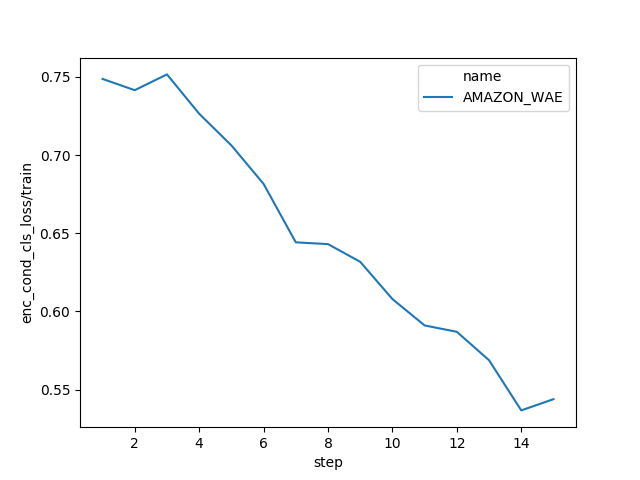
\includegraphics[width=1.\textwidth]{images/figs2/2020_01_15__11_37_34__enc_cond_cls_loss.png}
        \caption{}
        \label{fig:chap4:amazon_enc_cls}
    \end{subfigure}
    \begin{subfigure}{0.3\textheight}
        \centering
        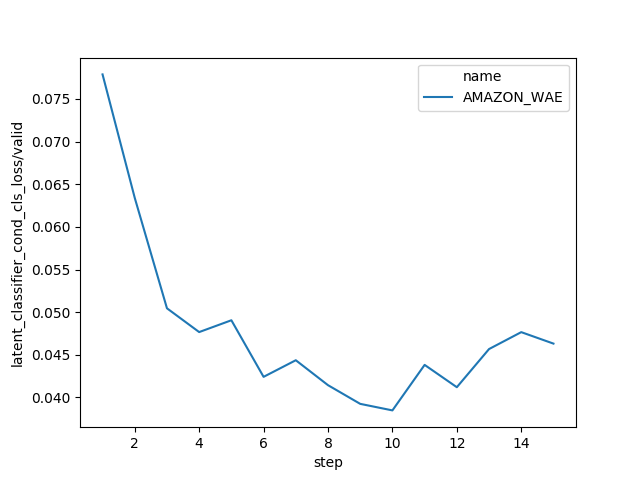
\includegraphics[width=1.\textwidth]{images/figs2/2020_01_15__11_37_34__latent_classifier_cond_cls_loss.png}
        \caption{}
        \label{fig:chap4:amazon_latent_cls}
    \end{subfigure}
    \begin{subfigure}{0.3\textheight}
        \centering
        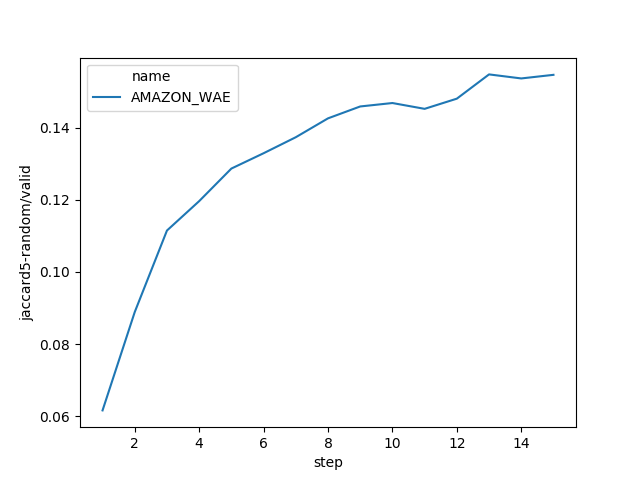
\includegraphics[width=1.\textwidth]{images/figs2/2020_01_15__11_37_34__jaccard5-random.png}
        \caption{}
        \label{fig:chap4:amazon_jaccard}
    \end{subfigure}
    \begin{subfigure}{0.3\textheight}
        \centering
        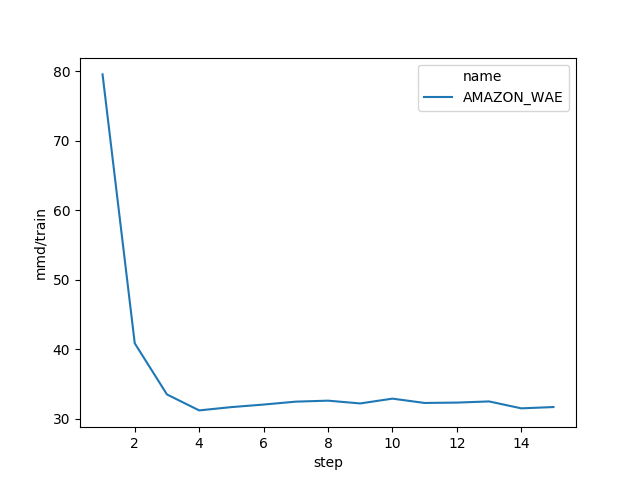
\includegraphics[width=1.\textwidth]{images/figs2/2020_01_15__11_37_33__mmd.png}
        \caption{}
        \label{fig:chap4:amazon_mmd}
    \end{subfigure}
    \begin{subfigure}{0.3\textheight}
        \centering
        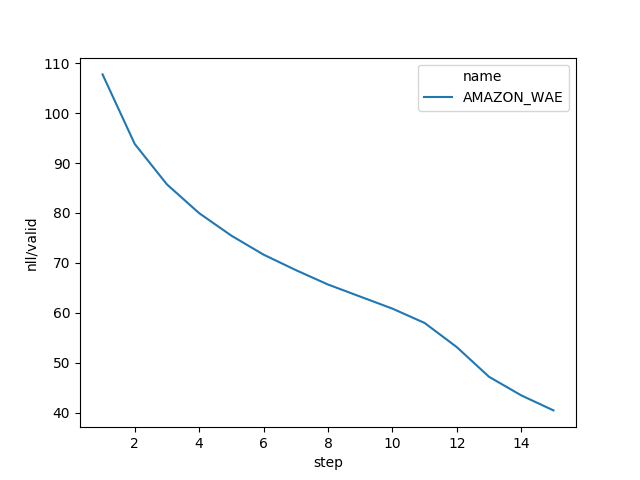
\includegraphics[width=1.\textwidth]{images/figs2/2020_01_15__11_37_34__nll.png}
        \caption{}
        \label{fig:chap4:amazon_nll}
    \end{subfigure}
    \caption{
        مدل پیشنهادی ۱.
        نمودار‌های آموزش \wae{} بر روی دادگان \amazon{}.
        هزینه دسته‌بندی بردار‌های نهان تولید شده توسط \encoder{}
        (\subref{fig:chap4:amazon_enc_cls})؛
        هزینه دسته‌بندی \classifier{} در فضای نهان
        (\subref{fig:chap4:amazon_latent_cls})؛
        کیفیت و تنوع جملات تولیدی با توجه به معیار \jaccard{}
        (\subref{fig:chap4:amazon_jaccard})؛
        فاصله توزیع \marginal{} \encoder{} و \priordist{} با توجه به معیار \mmd{}
        (\subref{fig:chap4:amazon_mmd})؛
        خطای بازسازی جملات
        (\subref{fig:chap4:amazon_nll}).
    }
    \label{fig:chap4:amazon_cond}
\end{figure}


\begin{figure}[h]
    \centering
    \begin{subfigure}{0.3\textheight}
        \centering
        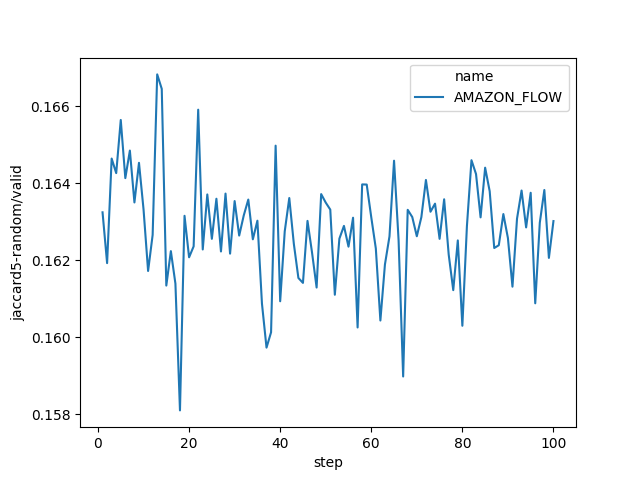
\includegraphics[width=1.\textwidth]{images/figs2/2020_01_15__11_41_02__jaccard5-random.png}
        \caption{}
        \label{fig:chap4:amazon_flow_jaccard}
    \end{subfigure}
    \begin{subfigure}{0.3\textheight}
        \centering
        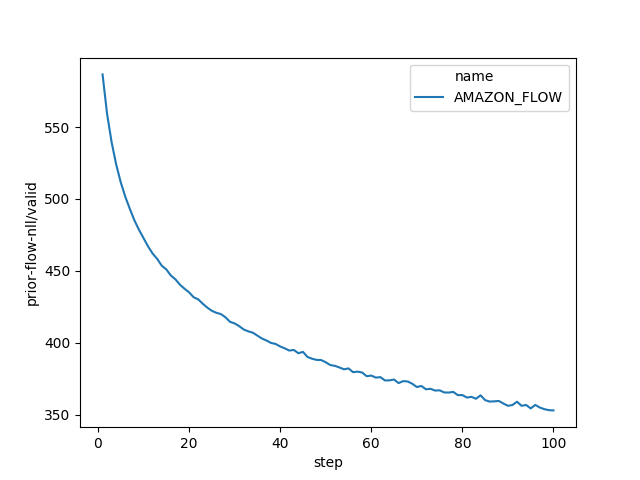
\includegraphics[width=1.\textwidth]{images/figs2/2020_01_15__11_41_01__prior-flow-nll.png}
        \caption{}
        \label{fig:chap4:amazon_flow_nll}
    \end{subfigure}
    \caption{
        مدل پیشنهادی ۱. نمودار‌های آموزش مولد شرطی بر روی دادگان \amazon{}.
        کیفیت و تنوع جملات تولیدی تولید شده توسط مدل مولد شرطی با توجه به معیار \jaccard{}
        (\subref{fig:chap4:amazon_flow_jaccard})؛
        تابع هزینه آموزش مولد شرطی
        (\subref{fig:chap4:amazon_flow_nll}).
    }
    \label{fig:chap4:amazon_flow}
\end{figure}

\begin{figure}[h]
    \centering
    \begin{subfigure}{0.3\textheight}
        \centering
        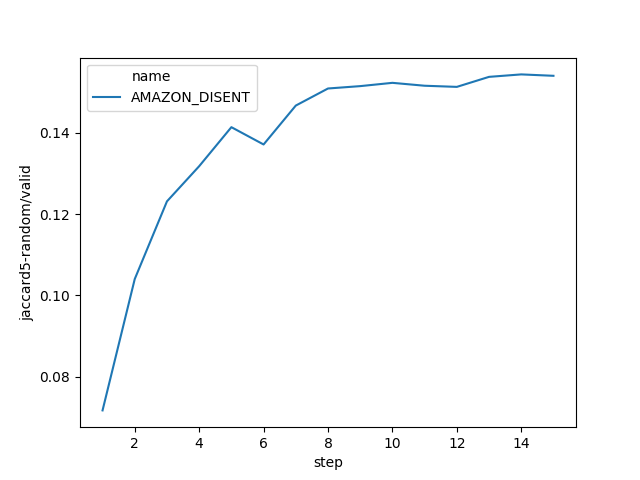
\includegraphics[width=1.\textwidth]{images/figs2/2020_01_15__11_42_11__jaccard5-random.png}
        \caption{}
        \label{fig:chap4:amazon_disent_jaccard}
    \end{subfigure}
    \begin{subfigure}{0.3\textheight}
        \centering
        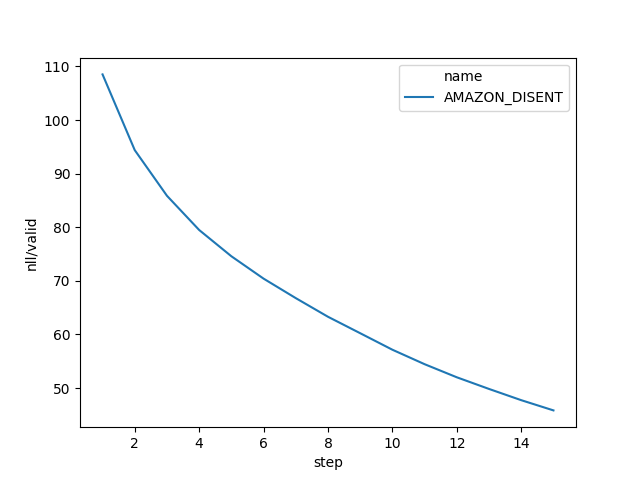
\includegraphics[width=1.\textwidth]{images/figs2/2020_01_15__11_42_11__nll.png}
        \caption{}
        \label{fig:chap4:amazon_disent_nll}
    \end{subfigure}
    \begin{subfigure}{0.3\textheight}
        \centering
        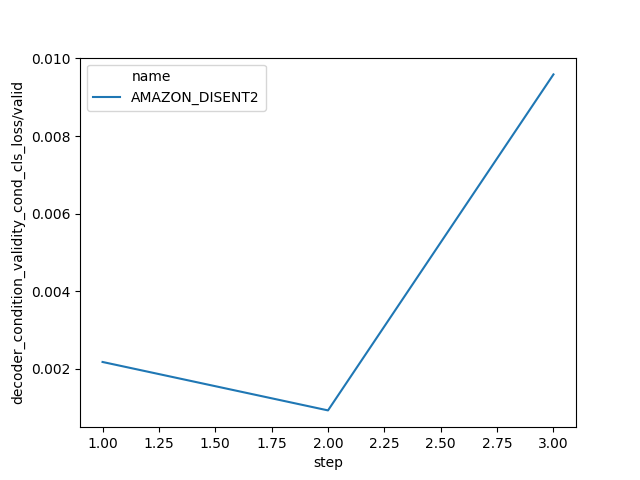
\includegraphics[width=1.\textwidth]{images/figs2/2020_01_15__12_10_34__decoder_condition_validity_cond_cls_loss.png}
        \caption{}
        \label{fig:chap4:amazon_disent_xcls}
    \end{subfigure}
    \begin{subfigure}{0.3\textheight}
        \centering
        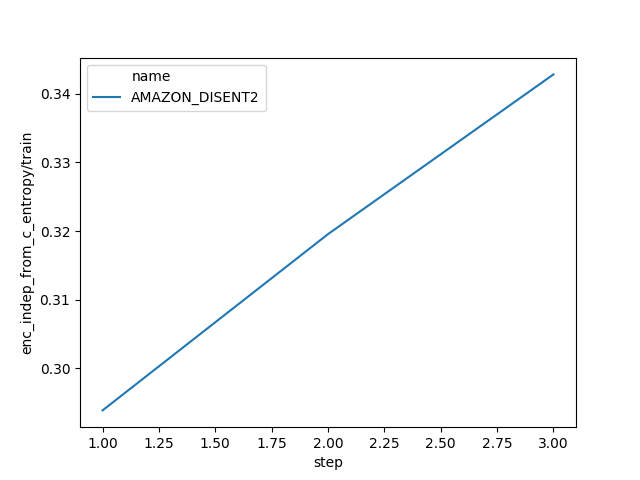
\includegraphics[width=1.\textwidth]{images/figs2/2020_01_15__11_44_04__enc_indep_from_c_entropy.png}
        \caption{}
        \label{fig:chap4:amazon_disent_indp}
    \end{subfigure}
    \begin{subfigure}{0.3\textheight}
        \centering
        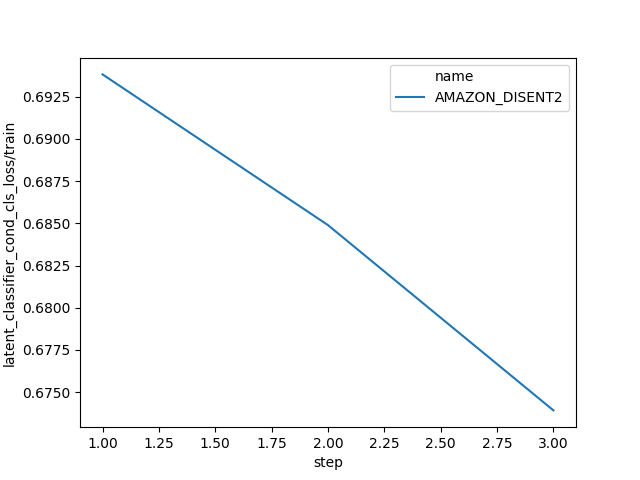
\includegraphics[width=1.\textwidth]{images/figs2/2020_01_15__11_44_04__latent_classifier_cond_cls_loss.png}
        \caption{}
        \label{fig:chap4:amazon_disent_latent_cls}
    \end{subfigure}
    \caption{
        مدل پیشنهادی ۲. نمودار‌های آموزش مدل بر روی دادگان \amazon{}.
        کیفیت و تنوع جملات تولیدی تولید شده توسط \decoder{} شرطی با توجه به معیار \jaccard{}
        (\subref{fig:chap4:amazon_disent_jaccard})؛
        خطای بازسازی
        (\subref{fig:chap4:amazon_disent_nll})؛
        تابع هزینه دسته‌بندی جملات
        (\subref{fig:chap4:amazon_disent_xcls})؛
        استقلال فضای نهان از شرط (آنتروپی \classifier{})
        (\subref{fig:chap4:amazon_disent_indp})؛
        استقلال فضای نهان از شرط (هزینه دسته‌بندی \classifier{} در فضای نهان)
        (\subref{fig:chap4:amazon_disent_latent_cls}).
    }
    \label{fig:chap4:amazon_disent}
\end{figure}

	%\chapter{آزمایش‌های بیشتر}\label{Chap:App3}
\minitoc
	%\include{Thesis_App3}
\end{appendices}
\bibliographystyle{ieeetr} %alpha or amsalpha or ieeetr. Control options of this style are put in IEEEtran_biboptions.bib file and activated just after \begin{document}
% IEEEtranSA
%\printglossaries
\cleardoublepage % terminates the current paragraph and page, the same way as a report document.
\phantomsection % hyperref: enable hyperlinking from the table of contents to this point
\addcontentsline{toc}{chapter}{مراجع} % add a line in the Table of Contents (first option, toc), it will be like the ones created by chapters (second option, chapter)
\renewcommand{\bibname}{\rl{مراجع}} % title of the bibliography chapter for the report and book styles. redefine \refname for the references section of an article
\chapter*{مراجع} % custom chapter, because in latin env, title goes LTR
{ %Disable chapter command for bibliography just in this block!
\renewcommand{\chapter}[2]{} % disable the automatic chapter
\begin{latin} % can use \setRTLbibitems in newer versions of xerpersian

\bibliography{IEEEabrv,Thesis_References} % IEEEtran_biboptions provides the customization options activated before by \bstctlcite
\end{latin}
}
% IEEEtran_biboptions,

%\makeglossaries
\cleardoublepage
\resettranslations
\printpersianglossary
\cleardoublepage
\printenglishglossary

\thispagestyle{empty} 
%\geometry{top=3cm,right=2.5cm,bottom=2.5cm,left=3.5cm} 

\begin{latin}
\centerline{\textbf{\large{Abstract}}}
\begin{quote}
    By the improvement of machine learning methods specially the Deep Learning in the last decade, there were expanding usage of these methods in Language Modeling task. As the essence of a language model is more basic, recently huge networks are trained with language model objective but fine-tuned on target tasks such as Question Answering, Sentiment Analysis and etc.
    which is a promising sign of its importance and usage in even other NLP tasks. However, this task still has severe problems. The Teacher Forcing based methods, suffer from the so-called exposure bias problem which is due to the train/test procedure discrepancy. Some solutions such as using Reinforcement Learning which has high variance or other approximate ones have been introduced. On the side of models with latent space, the ignorance of the latent space by the decoder is reported.
    \\
    The more practical task, Conditional Text Generation including determination of the tense of the output sentence or more complex conditions such as context or topic, has great importance. The usage of these models is not restricted to the text generation and they can be taken in account in creating drug molecules with specific characteristics, musics with specific genres or generating graphs with specific features. In conditional text generation, there will be additional problem which is the mismatch of generated sentence with the desired condition.
    \\
    In this project, a new approach in training conditional text generation with discrete conditions is proposed. The proposed method is a model with latent space while controlled the latent space ignorance problem and also partitioned the prior distribution on latent space with respect to the condition values. By incorporating the Normalizing Flow Networks, which have been recently in attention, the distribution of latent space of each condition is learnt.
    \\
    At the end, the baseline methods and the proposed method are evaluated against various metrics including quality, diversity and the match percentage of generated text with the desired condition. The proposed method outperforms the similar latent based method in some aspects.
\vskip 1cm
\textbf{Keywords: Conditional Text Generation, Generative Models with Latent Space, Neural Networks, Deep Learning} \textit{a}
\end{quote}
\end{latin}


\thispagestyle{empty}
\begin{center}
	\begin{latin}
		
\includegraphics{logo}
		
		\begin{large}
		Sharif University of Technology \\ \enDep{} 
		\vskip 0.8cm
		\enlevel{} \entype{} \\ \enmajor{}
		
		\end{large}
		\vskip 3cm
		{Topic}         \\ \large{ \textbf{\entitle}}
		\vskip 3 cm
		{By}         \\ \large{\enAuthor}
		\vskip 0.75 cm
		{Supervisor} \\ \large{\ensupervisor}
		\vskip 1cm
		\large{\engdate}
	\end{latin}
\end{center}


\thispagestyle{empty}
\cleardoublepage % terminates the current paragraph and page, the same way as a report document.
\end{document}
